
\documentclass[a4paper,11pt]{article}
% Maths resource packages
\usepackage{amsmath,amssymb,amsfonts,amsthm}
% Packages to allow inclusion of graphics
\usepackage{graphicx}
% For creating hyperlinks in cross references
\usepackage{hyperref}
% Literature reference style
\usepackage[authoryear]{natbib}
\usepackage[bf]{caption}



% -----------------------------
% --- user-defined commands ---
% -----------------------------

% insert Quantnet logo
\newcommand{\quantnet}{\raisebox{-1pt}{
\includegraphics[scale=0.05]{thesis/figures/qletlogo.pdf}}\,}

% --------------------------
% --- layout definitions ---
% --------------------------

% define topline
\usepackage[automark]{scrpage2}
\pagestyle{scrheadings}
\automark{section}
\clearscrheadings
\ohead{\headmark}

% define citation style
\bibliographystyle{ecta}

% define page size, margin size
\setlength{\headheight}{1.1\baselineskip}
\voffset=-2cm
\hoffset=-3cm
\textheight24cm
\textwidth15.5cm
\topmargin1cm
\oddsidemargin3cm
\evensidemargin3cm

% define line line spacing = 1.5
\renewcommand{\baselinestretch}{1.5}

% define second level for 'itemizing'
\renewcommand{\labelitemii}{-}



% --------------------------------------
% --------------------------------------
% --------------------------------------
% --- the structure this tex document ---
% frontmatter:
%   - titlepage,
%   - acknowledgement,
%   - abstract,
%   - table of contents,
%   - list of abbreviations,
%   - list of figures,
%   - list of tables.
%
% body of the thesis:
%   - introduction,
%   - methods,
%   - data,
%   - results,
%   - conclusion,
%   - literature,
%   - appendix (figures, tables).
%
% last page:
%   - declaration of authorship.
% --------------------------------------
% --------------------------------------
% --------------------------------------




\begin{document}

% -------------------------------
% --- frontmatter: Title page ---
% -------------------------------

\thispagestyle{empty}
\begin{center}

    {\Large{\bf Forecasting in blockchain-based smart grids: Solving a prerequisite for the implementation of local energy markets}} \vspace{1cm}


    {\normalsize Master's Thesis submitted\\\vspace{0.5cm}
    to}\\\vspace{0.5cm}
    {\normalsize{\bf Prof. Dr. Wolfgang H\"ardle}} \\\vspace{0.5cm}
    {\normalsize Humboldt-Universit\"at zu Berlin \\
    School of Business and Economics \\
    Ladislaus von Bortkiewicz Chair of Statistics} \vspace{1cm}
    
    
\includegraphics[]{thesis/figures/logo.pdf}
    \vspace{1cm}

    {\normalsize by \\\vspace{0.5cm}
    {\bf Michael Kostmann} \\
    (550961)} \vspace{1cm}


    {\normalsize in partial fulfillment of the requirements \\
    for the degree of \\
    {\bf Master of Science} \\\vspace{1cm}
    Berlin, \today}

\end{center}




% ------------------------------------
% --- frontmatter: Acknowledgement ---
% ------------------------------------
\newpage
\pagestyle{plain}
\pagenumbering{roman}   % define page number in roman style
\setcounter{page}{1}    % start page numbering
\section*{Acknowledgement}

I would like to thank Discovergy GmbH for the kind provision of their smart meter data.




% -----------------------------
% --- frontmatter: Abstract ---
% -----------------------------
\newpage
\section*{Abstract}
This document outlines a Master thesis topic. It summaries its relevance, background and related research, describes the data used, proposes methods, and exemplifies the research idea on a small data subsample.
The proposed research aims at implementing prerequisites for the employment of local energy markets on a distributed ledger technology. Such local energy markets have been described and simulated on a Blockchain in previous literature \cite[e.g.,][]{Mengelkamp:2018a}). However, the focus of previous literature has been on the problem of programming such a decentralized market platform in form of a Smart Contract . Fundamental prerequisites for this Smart Contract, such as reliable Smart Meter forecasts of households’ energy consumption and production, have been assumed as given. Thus, how forecasts with a reasonably small error can be computed, is neglected in this literature. This task is particularly challenging under the constraints imposed by the technical implementation of a market mechanism in a Smart Contract on a Blockchain.
Therefore, the proposed study aims to evaluate the possibility of providing such forecasts with existing forecasting methods and realistically available Smart Meter data. An extensive literature review of studies that use high-resolution Smart Meter data to predict individual household energy consumption was conducted. Based on these studies the following forecast-ing techniques seemed most promising and applicable to the task at hand: long short-term memory recurring neural networks (LSTM RNN), pooling-based deep recurring neural net-works (PD RNN), sparse autoregressive LASSO, and distinct wavelet transform (DWT) with Kernel-Wavelet-Functional prediction method (KWF). The best performing prediction technique in terms of four error measures (i.e., MAE, MAPE, NRSME, and MASE) will then be used to assess the effect of forecasting errors on the market mechanism described in \citet{Mengelkamp:2018a}.

%%%%%%%%%%%%%%%%%%%%%%%%%%%%%%%%%%%%%%%%%%%%%%%%%%%%%%%%%%%%%%%%%
This is the template for a thesis at the Chair of Econometrics of
Humboldt--Universit\"at zu Berlin. A popular approach to write a
thesis or a paper is the IMRAD method (Introduction, Methods,
Results and Discussion). This approach is not mandatory! You can
find more information about formal requirements in the booklet
`Hinweise zur Gestaltung der \"au\ss eren Form von Diplomarbeiten' which is available in the office of studies.

The abstract should not be longer than a paragraph of around 10 to 15 lines (or about 150 words). The abstract should contain a
concise description of the econometric/economic problem you
analyse and of your results. This allows the busy reader to obtain quickly a clear idea of the thesis content.




% -----------------------------
% --- frontmatter: Contents ---
% -----------------------------
\newpage
\tableofcontents
\clearpage


% ------------------------------------
% --- frontmatter: List of Figures ---
% ------------------------------------
\newpage
\addcontentsline{toc}{section}{List of Abbreviations}
\ohead[]{LIST OF ABBREVIATIONS}
\section*{List of Abbreviations}

\begin{tabular}{rp{0.2cm}lp{1cm}rp{0.2cm}l}
    CPI     & &  Consumer Price Index   & & ETF     & &  Equity Traded Funds  \\
    ETH     & &  Eat the Horse          & & XLM     & &  Xetra Liquidity
\end{tabular}




% ------------------------------------
% --- frontmatter: List of Figures ---
% ------------------------------------
\newpage
\addcontentsline{toc}{section}{List of Figures}
\ohead[]{\rightmark}
\listoffigures



% -----------------------------------
% --- frontmatter: List of Tables ---
% -----------------------------------
\newpage
\addcontentsline{toc}{section}{List of Tables}
\listoftables



% -------------------------------
% --- main body of the thesis ---
% -------------------------------
\newpage
\pagestyle{plain}
\setcounter{page}{1}    % start page numbering anew
\pagenumbering{arabic}  % page numbers in arabic style



\section{Introduction}\label{Sec:Intro}



%%%%%%%%%%%%%%%%%%%%%%
%%%   Motivation   %%%
%%%%%%%%%%%%%%%%%%%%%%

\subsection{Motivation}\label{Sec:Intro;Subsec:Motivation}

The increasingly wide-spread installation of renewable energy generators currently transforms the German energy landscape substantially \citep{Bayer:2018}. Already in 2016, almost 1.6 million photovoltaic micro-generation units were installed in Germany, according to the Bundesverband Solarwirtschaft \citep{BSW-Solar:2017}. This increasing amount of distributed renewable energy resources combined with a more volatile energy consumption of households – e.g., due to uncontrolled electric vehicle charging that can increase peak consumption \citep{Fitzgerald:2016,Floch:2017} – presents a serious challenge for grid operators. As in an electricity grid energy production and consumption always have to be balanced \citep{Weron:2006}, the increasingly volatile and hard to predict energy consumption and production in low voltage grids requires new technological solution to manage grid load and energy distribution.
Fortunately, the technological advancement, that lead to the increasing complexity in the energy landscape, also opens up new opportunities to increase the efficiency and reliability of distributed renewable energy production and distribution. As the amount of renewable energy production, that is fed into low voltage grids, has been increasing over the last years \citep{Bayer:2018}, it seems reasonable to shift part of the grid management to lower grid levels. While industry and research already established a comprehensive set of grid management solutions as well as sophisticated consumption and production forecasting techniques for highly aggregated levels, there is still little research on the same topics at lower aggregation levels, such as neighbourhoods or even individual households \citep{Meer:2018}.
One rather recent technological advancement that has the potential to increase the level of energy distribution efficiency on low aggregation level is the implementation of local energy markets on a distributed ledger technology, such as Blockchain. Blockchain has been called an invention similarly revolutionary and paradigm shifting as the Internet \citep{Swan:2015}. While much of the hype around Blockchain still has to stand the test against reality, the technology undeniably has the potential to enable new technological solutions. It is not for no reason that more than 20~\% of 70 surveyed German energy executives believe Blockchain will be “a game changer for the energy industry” and further 60~\% believe further dispersion of Blockchain technology is probable \citep{Burger:2016}. A use case that has been getting special attention due to the media-effective inauguration of the Brooklyn Microgrid \citep{newscientist:2016} is Blockchain-based local energy markets. Local energy markets (LEM) enable localized interconnected energy consumers, producers, and prosumers to trade locally produced energy on a market platform with a specific pricing mechanism \citep{Mengelkamp:2018a}. Major advantages of such local energy markets are (near) real-time pricing and balancing of energy production and consumption in local grids (ibid.). Blockchain-based LEM utilise a Blockchain as underlying information and communication technology and a Smart Contract to match supply and demand and settle transactions (ibid.).
However, the product traded on energy markets has some peculiarities compared to other markets. First, energy grids always have to be balanced, i.e. energy demand always has to be matched by energy supply \citep{Weron:2006}. Secondly, as energy is difficult to store, produced energy is fed into the grid mostly instantaneously and continuously and cannot be exchanged in batches of a specific amount at a single point in time. Traditionally, this means that the aggregated energy demand for a geographic area and a specific period of time has to be anticipated and according to this future demand energy is bought and sold. The actual electricity is then produced continuously matching the current demand. This setting is the reasons for today’s existing energy landscape, where utilities and large-scale energy producers and consumers are the only agents involved in electricity markets \citep{Weron:2006}. They trade energy according to the aggregated demand of many consumers. This aggregation makes forecasting future energy demand with relatively small errors \citep{Meer:2018, Wang:2018} and thereby efficient trading possible. Household-level consumers or prosumers, however, do not actively trade but pay their consumption or are reimbursed for their infeed of energy into the grid according to preset tariffs. In LEM, on the contrary, households are the participating market agents. Due to the peculiarities of energy trading mentioned above, the participating households need to forecast their energy demand, respectively supply, to be able to submit a buy or sell offer to the market. This forecasting is substantially harder for single households compared with higher aggregation levels \citep{Wang:2018}.
Therefore, the research outlined here aims to evaluate the possibility of providing such forecasts with existing forecasting methods and realistically available Smart Meter data. These forecasts are a necessary precondition for LEM and the blockchain-based LEM envisioned by \citet{Mengelkamp:2018a} in particular.

%%%%%%%%%%%%%%%%%%%%%%%%%%%%
%%%   Related research   %%%
%%%%%%%%%%%%%%%%%%%%%%%%%%%%

\subsection{Related research}\label{Sec:Intro;Subsec:Related}
The topic of concern for the research proposed touches upon two fields of research. The superordinate topic is local energy markets that are implemented on distributed ledger technology. A necessary prerequisite, that has to be fulfilled to be able to implement such Blockchain-based LEM, is the successful forecast of household-level energy consumption/production based on Smart Meter recordings. Without this, trading on the market mechanisms described in \citet{Block:2008} and implemented in a Smart Contract \citet{Mengelkamp:2018a} is not possible.


%%%%%%%%%%%
\subsubsection{Local energy markets}
While substantial work regarding LEM in general has been done \citep[e.g.,][]{Lamparter:2010,Li:2015, Mihaylov:2014}, there are only few examples of Blockchain-based LEM designs in the existing literature. 
\citet{Mengelkamp:2018b} derive seven principles for microgrid energy markets and evaluate the Brooklyn Microgrid according to those principles. According to the authors knowledge, they are the only ones providing a theoretical framework for the design of Blockchain-based LEM and their work may serve as the basis for the future research and implementation of such energy markets.
With a more practical focus, \citet{Mengelkamp:2018a} implemented and simulated a local energy market on a private Ethereum-Blockchain  that enables participants to trade local energy production on a decentralized market platform with no need for a central authority.
\citet{Münsing:2017} similarly elaborate a peer-to-peer energy market concept on a Blockchain but focus on operational grid constraints and a fair payment rendering. In doing so, they present a decentralized optimal power flow model suitable for implementation on a Blockchain.



%%%%%%%%%%%
\subsubsection{Blockchain and smart contracts}



%%%%%%%%%%%
\subsubsection{Local energy markets and blockchain technology}



%%%%%%%%%%%
\subsubsection{Load forecasting of single households}
As mentioned before, the simulations and concepts described in the research above rely on Smart Meters capable of forecasting the expected energy consumption or production of a household for the next trading interval. This forecasting task is not trivial due to the extremely high volatility of individual private energy consumption \citep{Wang:2018}. Nevertheless, there are several studies trying to forecast different time horizons of Smart Meter time series.
\citet{Arora:2016} compute probability density estimates for the electricity consumption recorded by individual Smart Meters in halfhourly intervals from 1000 households and SMEs in Ireland over the course of one year. They employ unconditional and conditional kernel density estimators with a decay parameter to generate point and density forecasts for electricity consumption from 30 minutes to one week ahead.
\citet{Kong:2018} use a long shortterm memory deep learning framework to make one time-step ahead forecasts on the AMPds dataset containing half-hourly recordings of energy and appliance usage measurements of a single household in Canada. They show that the prediction accuracy can be improved substantially by including appliance measurement data.
Contrary to this machine learning approach, \citet{Li:2017} use statistical methods to make one time-step ahead forecasts with a sparse autoregressive LASSO model. Using a dataset of 150 consumers from PG\&E with hourly energy consumption recordings for one year, their model captures sparsity in the household’s historical data via LASSO to make a prediction for one household. This prediction is further improved with the historical consumption data of one additional household. This household is identified with the help of a covariance statistic test to identify one other household’s data has the best predictive leverage to improve the original forecast.
On the same dataset as \citet{Arora:2016}, \citet{Shi:2017} use a pooling-based deep recurring neural network to make point forecasts of future consumption and achieve substantial mean absolute percentage error (MAPE) reductions compared to ARIMA, recurring neural network, support vector machine, and deep recurring neural network approaches.
Even though focusing on the forecast of aggregated energy consumption, the work of \citet{Zufferey:2017} shows promising results for forecasting Smart Meter time series with time delay neural networks (TDNN) using mostly historical features of the time series itself. They use a huge dataset of 40.000 small consumers and 400 photovoltaic power generators in Basel, Switzerland with 15-minute interval recordings of energy consumption and production for one year.
A comprehensive overview on the state of the art of Smart Meter data analytics is provided by \citet{Wang:2018}. They not only focus on studies researching load forecasting but also provide comprehensive insights into studies regarding Smart Meter data clustering, preprocessing, load analysis and more. Furthermore, they provide a summary of publicly available Smart Meter datasets and open research topics.
Notably, there is a lack of standard regarding which forecasting error measures are reported and what benchmark models are used in Smart Meter data forecasting studies. This is also pointed out by \citet{Meer:2018} in their review paper on probabilistic consumption and production forecasting. Due to this, different forecasting techniques employed in studies using different datasets with partly differing objectives are not directly comparable. Which forecasting techniques should be used in the research proposed here is therefore not directly inferable from the success in applying different forecasting techniques in previous studies.



%%%%%%%%%%%%%%%%%%%%%%%%%%%%
%%%   Present research   %%%
%%%%%%%%%%%%%%%%%%%%%%%%%%%%
\subsection{Present research}\label{Sec:Intro;Subsec:Present}



%%%%%%%%%%%
\subsubsection{Objective}
The aim of the proposed Master thesis is to investigate the prerequisites necessary to implement Blockchain enabled distributed energy markets. In particular this is,
a)	forecasting net energy consumption/production of private consumers and prosumers one time-step ahead based only on their historical consumption/production data,
b)	evaluate and quantify the effects of forecasting error for participating households, and
c)	evaluate the implications of variations in forecasting quality for a market mechanism including penalties for forecast-actual consumption/production deviations.
The underlying setting and technical implementation of the local energy market, that is assumed for the proposed research, is provided by \citet{Mengelkamp:2018a}. The prediction task is fitted to their setup of a local energy market that uses Blockchain technology as its information and communication medium and thereby, the proposed study distinguishes itself notably from previous studies trying to forecast Smart Meter time series. Likewise, the evaluation of forecasting errors and their implications is based on their described market mechanism and penalty structure and has as such to the authors knowledge not been done in other studies.


%%%%%%%%%%%
\subsubsection{Research questions}
The following research questions are intended to be answered in the proposed Master thesis:
a)	Which prediction technique yields the best 15-minute ahead forecast  for Smart Meter time series measured in 3-minute intervals using only input features generated from the historical values of the time series and calendar-based features?
b)	Assuming a penalty structure as described in \citet{Mengelkamp:2018a}, what is the quantified loss of households participating in the local energy market due to forecasting errors by the prediction technique identified in a)?
c)	Depending on the results from b), what implications and potential adjustments for the market mechanism described in \citet{Mengelkamp:2018a} can be identified?



%%%%%%%%%%%%%%%%%%%%%%%%%%%%%%%%%%%%%%%%%%%%%%%%%%%%%%%%%%%%%%%%%

\begin{itemize}

    \item What is the subject of the study? Describe the
        economic/econometric problem.

    \item What is the purpose of the study (working hypothesis)?

    \item What do we already know about the subject (literature
        review)? Use citations: {\it \cite{Gallant:87} shows that...
        Alternative Forms of the Wald test are considered
        \cite{Breusch&Schmidt:88}.}

    \item What is the innovation of the study?

    \item Provide an overview of your results.


    \item Outline of the paper:\\
        {\it The paper is organized as follows. The next section describes the
        model under investigation. Section~\ref{Sec:Data} describes the data set
        and Section~\ref{Sec:Results} presents the results. Finally, Section
        ~\ref{Sec:Conc} concludes.}

    \item The introduction should not be longer than 4 pages.

\end{itemize}


\section{Methods}\label{Sec:Method}

Based on the extensive literature review briefly presented above, two different forecasting techniques were chosen to be employed to predict households' energy consumption and production. The following criteria were considered for the selection of appropriate methods: 

\begin{enumerate}
    \item The forecasting technique had to produce deterministic (i.e., point) forecasts.
    \item The forecasting technique had to be used in existing studies about forecasting energy consumption or production.
    \item The existing study or studies using the forecasting technique had to use comparable data, i.e., recorded by smart meters, 60-min or higher resolution, recorded in multiple households, and not recorded in SMEs or other business or public buildings.
    \item The forecasting task had to be comparable to the forecasting task of this study, i.e., single consumer household (in contrast to the prediction of aggregated energy time series) and very short forecasting horizon ($\leq 24$ hours).
    \item The forecasting technique had to only take historical and calender features as input for the prediction.
    \item The forecasting technique had to produce absolutely and relative to other studies promisingly accurate predictions.
\end{enumerate}

\noindent Based on these criteria two forecasting techniques were selected for the prediction task at hand. As short-term energy forecasting techniques are commonly categorized into statistical and machine learning (or artificial intelligence) methods \citep{Bansal:2015,Diagne:2013,Gan:2017}, one method of each category was chosen: Deep recurrent neural network (DRNN) adapted from the procedure outlined by \citet{Shi:2017} and sparse autoregressive LASSO as developed and implemented by \citet{Li:2017}.%, and Kernel-Wavelet-Functional method (KWF) following the idea of \citet{Auder:2018} of using discrete wavelet transform and clustering before applying the KWF method.

Before these two methods are explained in detail, the benchmark model, that serves as a baseline for the assessment of the prediction methods, is presented next.


%%%%%%%%%%%%%%%%%%%%%%%%%%%
%%%   Benchmark model   %%%
%%%%%%%%%%%%%%%%%%%%%%%%%%%

\subsection{Benchmark model} \label{Sec:Method;Subsec:Benchmark}

Benchmark models serve as a trivial baseline to assess the relative improvement of a sophisticated model \citep{Meer:2018}. According to \citet{Pinson:2012}, a benchmark model should serve as a reference, need few computational resources to be estimated, and be model-free. A sophisticated forecasting method is only worth implementing if it can significantly outperform a trivial benchmark model \citep{Diagne:2013}. A frequent benchmark model used for deterministic forecasts is the simple persistence model \citep{Meer:2018}. This model assumes that the conditions at time $t$ persist at least up to the period of forecasting interest at time $t+h$. In energy forecasting, this na\"ive model is surprisingly well suited to forecast very short time periods of a few seconds or minutes \citep{Pinson:2012} and, thus, often harder to beat than it might seem. Here, the persistence model is defined as
%
\begin{equation} \label{Eq:naivepred}
\widehat{x}_{t+1}=x_t.
\end{equation}

There are several other benchmark models commonly used in energy load forecasting. Most of them are, in contrast to the persistence model, more sophisticated benchmarks, such as the Holt-Winters-Taylor (HTW) exponential smoothing method \citep[see, e.g.,][]{Arora:2016}. Further sophisticated benchmark models are the Vanilla benchmark \citep{hong:2010}, and the popular ARMA method \citep{Box:1990}. However, as the forecasting task at hand serves the specific use case of being an input for the bidding process in a blockchain-based local energy market, the improvement of the forecasting model over a benchmark model is of secondary importance. The task here is not so much to establish the quality of a forecasting model per se as to assess whether the available and most promising forecasting techniques can deliver accurate enough results for the use case explained above. Hence, only the persistence model will serve as a benchmark to the forecasting techniques presented next. The more relevant test of the forecasting models' accuracy will be explained in Section~\ref{Sec:Method;Subsec:Market}.



%%%%%%%%%%%%%%%%
%%%   LSTM   %%%
%%%%%%%%%%%%%%%%

\subsection{Machine learning based forecasting approach} \label{Sec:Method;Subsec:LSTM}

The first sophisticated forecasting technique that is employed to produce accurate predictions for the blockchain-based LEM is a machine learning algorithm. Even though being applied very successfully in a wide range of tasks, such as speech recognition \citep{Graves:2013} or anomaly detection in time series \citep{Malhotra:2015}, long short-term memory (LSTM) neural networks (NN) have been introduced only very recently in load forecasting studies \citep[e.g.,][]{Kong:2018,Shi:2017,Gan:2017,Chen:2018}. Compared to previous attempts using machine learning techniques, the applications of LSTM neural networks for load forecasting have been much more successful \citep{Kong:2018,Shi:2017}. This is most likely due to the high effectiveness of recurrent neural networks for sequence learning. LSTM neural networks are a advanced architecture of recurrent neural networks that are particularly well suited to learn long sequences or time series due to their ability to retain information over many time steps. The next three sections explain the basic working principles of the chosen machine learning approach and are based on \citet{chollet:2018}, \citet{Lipton:2015}, and \citet{Gan:2017}.



%%%%%%%%%%%
\subsubsection{Basic functioning of neural networks}

To understand the full advantage that LSTM recurrent neural networks have over other machine learning techniques for time series learning, it is useful to take a step back and recapitulate the basic functioning of a so-called feedforward neural network. Neural networks do not need any strong assumptions about their functional form, such as traditional time series models (e.g., ARMA). Still, they are universal approximators for finite input \citep{Hornik:1989} and, therefore, especially well suited for the prediction of such volatile time series as energy consumption or production. The most basic building blocks of any neural network are three types of layers: an input layer, one or more hidden layer(s), and an output layer. Each layer consists of one or more units (sometimes called neurons). Each unit in a layer takes in an input, applies a transformation to this input, and outputs it to the next layer (see Figure~\ref{Fig:simpleNN}). Formally, this can be written as
%
\begin{equation} \label{Eq:feedforward}
\begin{split}
    \vec{h}_{1,i}&=\phi_1\left(\vec{W}_1\vec{x}_i+\vec{b}_1\right)\\
    \vec{h}_{2,i}&=\phi_1\left(\vec{W}_2\vec{h}_{1,i}+\vec{b}_2\right)\\
    &\setbox0\hbox{=}\mathrel{\makebox[\wd0]{\hfil\vdots\hfil}}\\
    o_i&=\phi_n\left(\vec{W}_n\vec{h}_{(n-1),i}+\vec{b}_n\right)=\widehat{y}_i,
\end{split}
\end{equation}
%
where $n$ denotes a layer, $\phi_n$ is the activation function, $\vec{W}_n$ is the weight matrix, and $\vec{b}_n$ the bias vector in layer $n$. $\vec{x}_i$ is the $i^{th}$ input vector and $o_i$ the output value of the output layer which is the estimation of the true value $y_i$.
%
\begin{figure}[htbp]
    \centering
    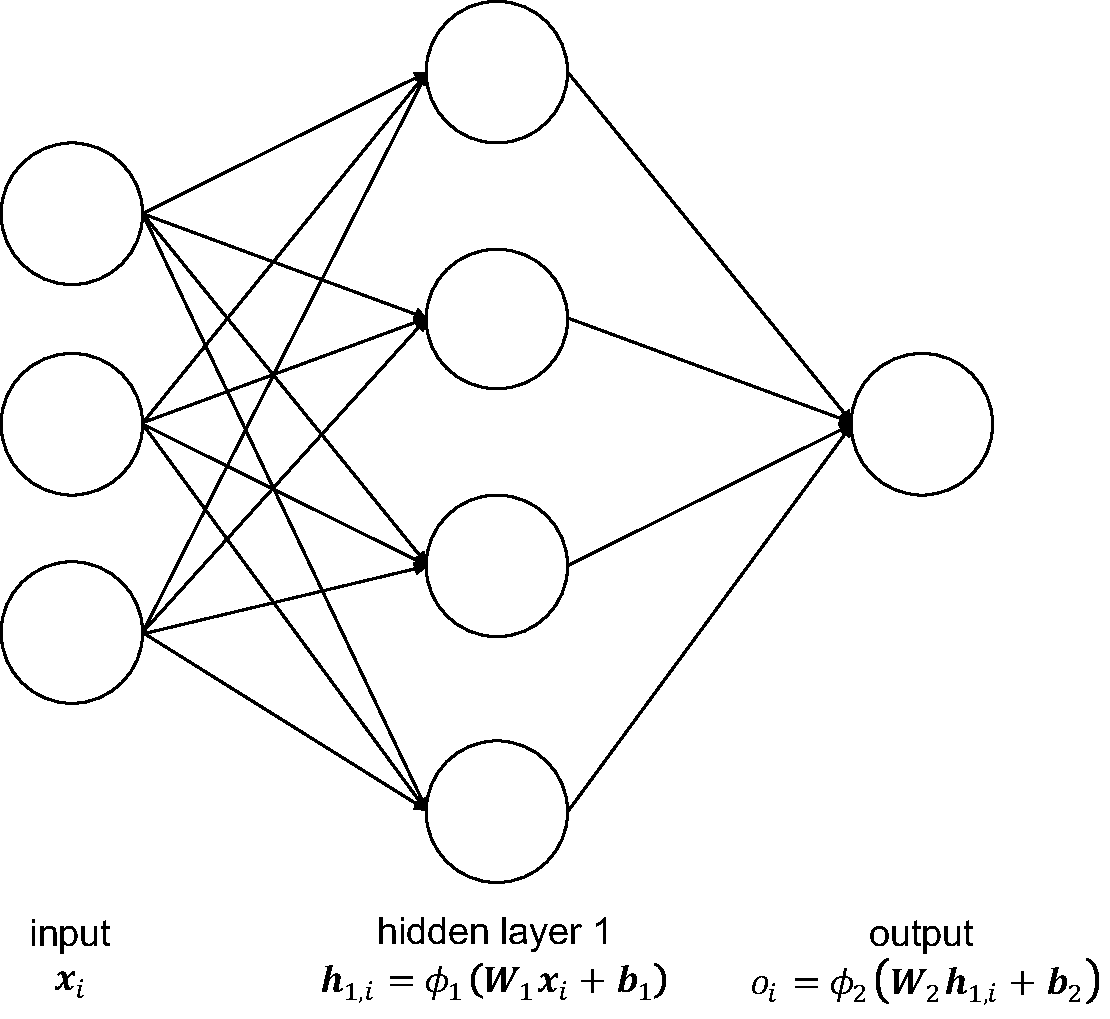
\includegraphics[scale=0.5]{thesis/figures/simpleNN.pdf}
    \caption[Schematic representation of a simple neural network]{Schematic representation of a simple neural network. Adapted from \citet{Gan:2017}.}
    \label{Fig:simpleNN}
\end{figure}

In the input layer there are as many units as there are features (i.e., variables) that serve as input for the forecasting model. The units of the input layer are connected to all units in the (first) hidden layer. The weight matrices and bias vectors in each layer are parameters that are adjusted during the training of the model. In all subsequent hidden layers, all units of one layer are connected to all units of the next layer (this is called densely connected). The last layer consists of as many units as there are output values. That is, if the forecasting model should just predict a single value, the output layer will have a single unit that takes in the weighted output values of all units of the last hidden layer, applies a transformation to these inputs and outputs a single value. The transformation that is applied to the input within each unit is called activation function and must be chosen depending on the task at hand. Especially for sequence learning, this activation function is often a hypberbolic tangent (tanh) \citep{Lipton:2015}:

\begin{equation} \label{Eq:activation}
    \phi(z)=\frac{e^z-e^{-z}}{e^z+e^{-z}}.
\end{equation}

The learning in machine learning refers in the case of neural networks to adjusting the weight matrices and bias vectors such that the best prediction is output. In supervised learning, adjusting these weights (i.e., the training of the model) is done through an algorithm that is called backpropagation which was introduced by \citet{Rumelhart:1986}. First, the weight matrices and bias vectors are randomly initialized. Then, in a first iteration, the training data is fed into the network, which outputs a prediction. This prediction is assessed with the help of a loss function that quantifies the distance between the prediction and the true value. A commonly used loss function is the mean absolute error:
%
\begin{equation} \label{Eq:lossMAE}
    L\left(y, \widehat{y}\right)=\text{MAE}=\frac{1}{N}\sum_{i=1}^N\left|\widehat{y}_i-y_i\right|
\end{equation}
%
The simplest method to optimize the model parameters is to compute the derivative of the loss function with respect to each parameter in the model and change each parameters in a fixed-size step in the direction of the negative gradient \citep{Graves:2013}. This method is called gradient descent. Thereby the prediction error is ``backpropagated" through the network to update the parameters. This is repeated in each iteration until the model converges to a value of the loss function that cannot be further improved.



%%%%%%%%%%%
\subsubsection{Recurrent neural networks}

Unfortunately, feedforward neural networks are not particularly well-suited for time series learning \citep{chollet:2018}. This is because simple neural networks, such as the one described above, do not have an internal state that could retain a memory of previously processed input. That is, to learn a sequence or time series, a feedforward neural network would always need the complete time series as a single input. It cannot retain a memory of something learned in a previous chunk of the time series to apply it to the next chunk that is fed into the model. This problem is tackled by recurrent neural networks.

Recurrent neural networks still consist of the basic building blocks of units and layers. However, the units do not just feed forward the transformed input as output but have a recurrent connection that feeds an internal state back into the unit as input (see Figure~\ref{Fig:RNNunit}). Thereby, a RNN unit loops over individual elements of an input sequence, instead of processing the whole sequence in a single step. This means, the RNN unit applies the transformation to the first element of the input sequence and combines it with its internal state. This introduces the notion of time into neural networks. Formally, this can be written as
%
\begin{equation} \label{Eq:RNN}
\begin{split}
    \vec{h}_{1,t}&=\phi_1\left(\vec{W}_1^{(i)}\vec{x}_t+\vec{W}^{(r)}_1\vec{h}_{1,(t-1)}+\vec{b}_1\right)\\
    \vec{h}_{2,t}&=\phi_2\left(\vec{W}_2^{(i)}\vec{h}_{1,t}+\vec{W}^{(r)}_2\vec{h}_{2,(t-1)}+\vec{b}_2\right)\\
    &\setbox0\hbox{=}\mathrel{\makebox[\wd0]{\hfil\vdots\hfil}}\\
    o_t&=\phi_n\left(\vec{W}_n^{(i)}\vec{h}_{(n-1),t}+\vec{b}_n\right)=\widehat{y}_t,
\end{split}
\end{equation}
%
where $n$ denotes a layer, $\phi_n$ is the activation function, $\vec{W}_n^{(i)}$ is the weight matrix for the input, $\vec{W}_n^{(r)}$ is the weight matrix for the recurrent input (i.e., the output of layer $n$ in the previous time step), and $\vec{b}_n$ the bias vector in layer $n$. $\vec{x}_t$ is the input vector at time $t$ and $o_t$ the output value of the output layer which is the estimation of the true value $y_t$. Note that the output layer has no recurrent units but is the same as in a simple feed forward network.
%
\begin{figure}[htbp]
    \centering
    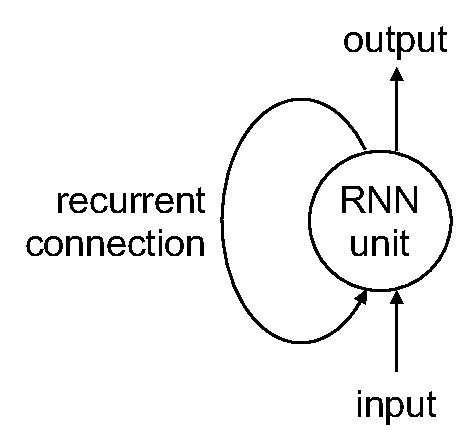
\includegraphics[scale=0.5]{thesis/figures/RNNunit.pdf}
    \caption[Schematic representation of a RNN unit]{Schematic representation of a RNN unit. Adapted from \citet{chollet:2018}.}
    \label{Fig:RNNunit}
\end{figure}

The cyclical structure of an RNN unit can be unrolled across time (see Figure~\ref{Fig:RNNunfolded}). This illustrates that a RNN is basically a simple neural network that has one layer for each time step that has to be processed per input. This notion of an unfolded RNN also reveals, that a RNN is still trainable through backpropagation. The backpropagation just has to happen across all time steps. This is called backpropagation through time (BPTT) and was introduced by \citet{Werbos:1990}. Theoretically, this feedback structure enables RNN to retain information about sequence elements that have been processed many steps before the current step and use it for the prediction of the current step. However, in practice the vanishing gradient problem occurs\footnote{For more details on the vanishing gradient problem see, e.g., \citet{Bengio:1994}}. This problem makes RNNs for very long sequences basically untrainable.
%
\begin{figure}[htbp]
    \centering
    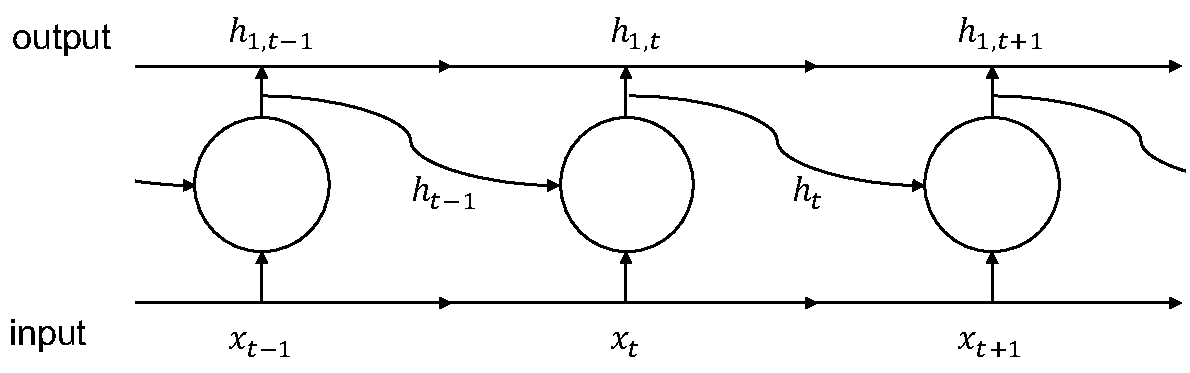
\includegraphics[scale=0.6]{thesis/figures/RNNunfolded.pdf}
    \caption[Schematic representation of an unfolded RNN unit]{Schematic representation of an unfolded RNN unit. Adapted from \citet{chollet:2018}.}
    \label{Fig:RNNunfolded}
\end{figure}



%%%%%%%%%%%
\subsubsection{Long short-term memory units}

To overcome the vanishing gradient problem, \citet{Hochreiter:1997} developed LSTM units. LSTM units extend RNN units by an additional state. This state can retain information for as long as needed. In which step this additional state is updated and in which state the information it retains is used in the transformation of the input is controlled by three so-called gates\footnote{In their original specification, \citet{Hochreiter:1997} included only two gates. However, as this LSTM specification was still prone to the vanishing gradient problem under some circumstances, \citet{Gers:2000} extended it by a third gate.}. These three gates again have the form of a simple RNN cell. Formally, the gates can be written as (following the notation of \citet{Lipton:2015}\footnote{\cites{Lipton:2015} notation uses $h_{t-1}$ instead of $s_{t-1}$. The notation used here ($s_{t-1}$) accounts for the modern LSTM architecture with peephole connections. For more information see \cite{Gers:2002}.})
%
\begin{equation} \label{Eq:LSTMgates}
\begin{split}
    \vec{i}_t&=\sigma\left(\vec{W}^{(ix)}\vec{x}_t+\vec{W}^{(is)}\vec{s}_{t-1}+\vec{b_i}\right)\\
    \vec{f}_t&=\sigma\left(\vec{W}^{(fx)}\vec{x}_t+\vec{W}^{(fs)}\vec{s}_{t-1}+\vec{b_f}\right)\\
    \vec{o}_t&=\sigma\left(\vec{W}^{(ox)}\vec{x}_t+\vec{W}^{(os)}\vec{s}_{t-1}+\vec{b_o}\right),
\end{split}   
\end{equation}
%
where $\sigma$ is the sigmoid activation function $\sigma(z)=\frac{1}{1+e^{-z}}$, $W$ denotes the weight matrices that are intuitively labeled ($ix$ for the weight matrix of gate $i_t$ multiplied with the input $x_t$ etc.), and $b$ denotes the bias vectors.\footnote{Sometimes, the gates are titled input, output, and forget gate. However, as \citet{chollet:2018} put it:
\vspace{0.75\dimexpr-\topsep-\partopsep}
\begin{quote}
    ``[T]hese interpretations don’t mean much, because what these [gates] actually do is determined by the contents of the weights parameterizing them; and the weights are learned in an end-to-end fashion, starting over with each training round, making it impossible to credit this or that operation with a specific purpose" (p. 193).
\end{quote}\vspace{\dimexpr-\topsep-\partopsep}
}

Again following the notation of \citet{Lipton:2015}, the full algorithm of a LSTM unit is given by the three gates specified above, the input node
%
\begin{equation} \label{Eq:LSTMinput}
    \vec{g}_t=\sigma\left(\vec{W}^{(gx)}\vec{x}_t+\vec{W}^{(gh)}\vec{h}_{t-1}+\vec{b_g}\right),
\end{equation}
%
the internal state of the LSTM unit at time step $t$
%
\begin{equation} \label{Eq:LSTMstate}
    \vec{s}_t=\vec{g}_t\odot\vec{i}_t+\vec{s}_{t-1}\odot\vec{f}_t,
\end{equation}
%
where $\odot$ is pointwise multiplication, and the output at time step $t$
%
\begin{equation} \label{Eq:LSTMoutput}
    \vec{h}_t=\phi\left(\vec{s}_t\right)\odot\vec{o}_t.
\end{equation}
%
The internal structure of a LSTM cell is further clarified by Figure~\ref{Fig:LSTMunit}. For an intuitive but more detailed explanation of LSTM neural networks see \citet[][Ch. 6.2]{chollet:2018}
%
\begin{figure}[htbp]
    \centering
    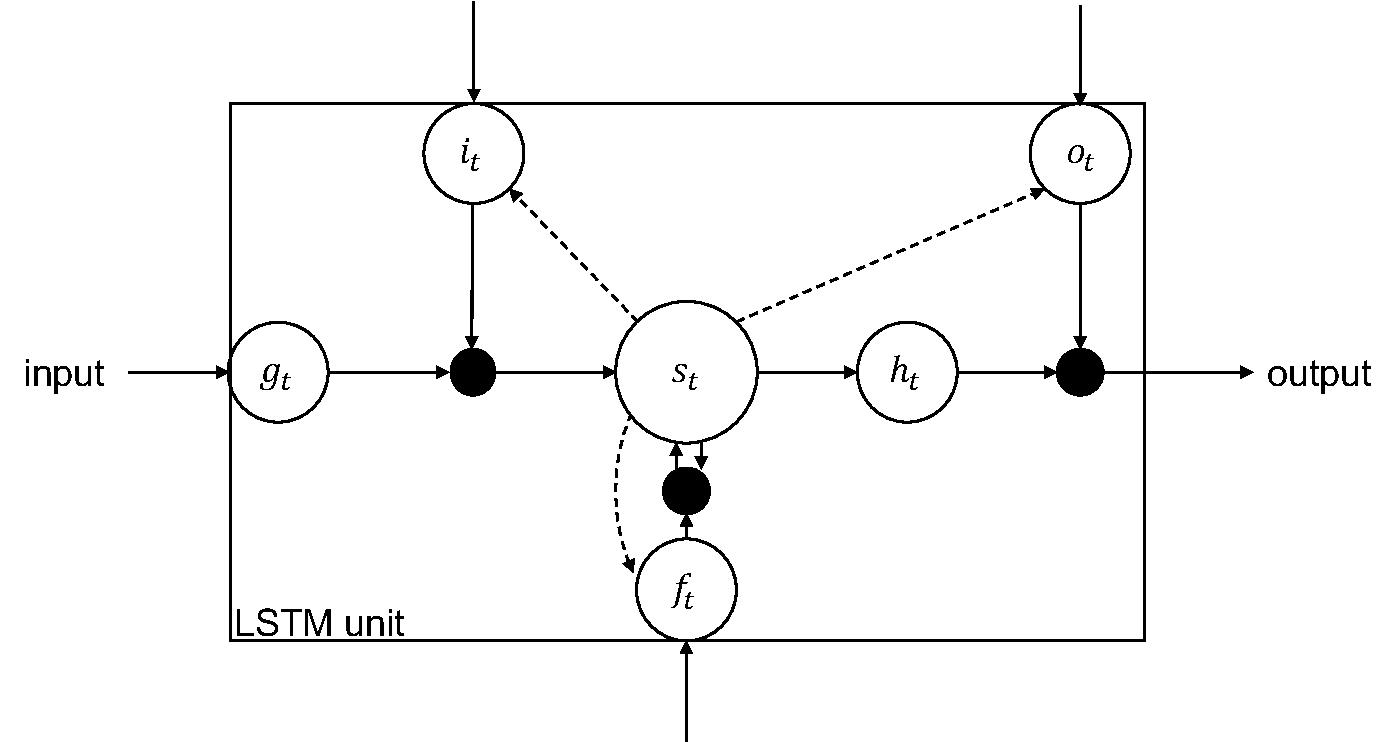
\includegraphics[scale=0.5]{thesis/figures/LSTMunit.pdf}
    \caption[Schematic representation of a LSTM unit]{Schematic representation of a LSTM unit. Adapted from \citet{Graves:2012}. The filled in circles represent the pointwise multiplication operation denoted by $\odot$ in Equation~\ref{Eq:LSTMstate} and~\ref{Eq:LSTMoutput}.}
    \label{Fig:LSTMunit}
\end{figure}

To summarize, all neural networks use the basic building blocks of units that form input, hidden, and output layers. The training process of neural networks involves updating the parameters (weights and biases) of the model based on the gradient descent of a loss function that quantifies the accuracy of a prediction compared to true values. RNN enables the neural network to process individual elements of a sequence or time series sequentially and still use information that was obtained in previous time steps for the current transformation of the input. LSTM RNN is an extension of simple RNN which has the advantage of being able to retain a state over multiple time steps and solves the vanishing gradient problem through the introduction of an additional internal state $\vec{s}_t$. By this, LSTM RNN are capable of learning highly complex, non-linear relationships in time series data which makes them a promising forecasting technique to predict households' very short-term energy consumption and production.



%%%%%%%%%%%
\subsubsection{Implementation of LSTM RNN}

The specific LTSM RNN approach adopted in this study is based on the procedure employed by \citet{Shi:2017} to forecast individual households' energy consumption. However, according to the relevant use case in this study, model training and predictions were performed using only the data of individual households. That means, a LSTM recurring neural network was trained for each household individually using only the households historic consumption patterns and calender features. This differs from \cites{Shi:2017} implementation, that used pooled consumption data of multiple households. Specifically, seven weeks of past consumption, an indicator for weekends, and an indicator for Germany-wide holidays were used as input for the neural network in the present study. The target values were single consumption values in 15-minute aggregation. Take the following example as illustration: The consumption values in 3-minute intervals from 13.11.2017 13:00 until 20.11.2017 13:00 and zero/one-indicators for weekends and holidays (i.e., 3 $\times$ 3360 data points) are fed into the neural network. The model then produces a single output value that estimates the household's energy consumption in kWh from 20.11.2017 13:00 until 20.11.2017 13:15.

A neural network is defined by several so-called hyperparameters: The number and type of layers, the number of hidden units within each layer, the activation functions used within each unit, dropout rates for the recurrent transformation, and dropout rates for the transformation of the input. These hyperparameters must be chosen particularly for the task at hand and their influence on the model performance is difficult to foresee. For this reason, parameter tuning was employed to find a relatively well working combination of hyperparameter values. Unfortunately, hyperparameter tuning is computationally very resource intensive as for each hyperparameter combination, the model must be fully trained to asses the model performance. Hence, not all possible or sensible combinations of hyperparameters could be assessed. Instead, a random sample of different hyperparameter combinations was chosen and the resulting model configurations trained and evaluated on a randomly chosen data set.

Table~\ref{Tab:LSTMHyperparameters} presents the hyperparameters that were tuned and their respective value ranges. The tuning was done individually for each layer. First layer 1 hyperparameters were tuned. The best found hyperparameter combination was then fixed for layer 1 and the parameters for layer 2 were tuned. This was repeated for layer 3. Optimally, all hyperparameters should be tuned simultaneously. However, due to computational constraints, that was not possible here and, thus, the described, second-best option chosen. As the hyperparameter values specified in Table~\ref{Tab:LSTMHyperparameters} for layer 1 alone result in 81 possible hyperparameter combinations, only samples of these combinations were taken, the resulting models trained and compared. In total, 16 models with one layer, 13 models with two layers and 13 models with 3 layers were tuned. The model tuning was conducted on the Machine Learning (ML) Engine of the Google Cloud Platform. The job was submitted to The ML Engine via Google Cloud SDK and the R package \texttt{cloudml}. The model training was conducted on four Tesla P100 GPUs. The necessary credits to pay for the hardware resources were granted by Google as part of their Google Cloud Platform Free Tier program\footnote{For further details see \url{https://cloud.google.com/free} (last accessed 01.10.2018).}.

\begin{table}[htbp]
    \begin{center}
        {\footnotesize
        \begin{tabular}{l|lcccc}
        \hline \hline
        & \multirow{2}{3em}{hyperparameter} & possible & possible     & sampling & \# of assessed \\
        &                                   & values   & combinations & rate     & combinations   \\
        \hline
                \multirow{4}{3em}{layer 1}  & batch size        & \{128, 64, 32\} & \multirow{4}{1em}{81} & \multirow{4}{1em}{0.2} & \multirow{4}{1em}{16} \\
                                            & hidden units      & \{128, 64, 32\} & & &\\
                                            & recurrent dropout & \{0, 0.2, 0.4\} & & & \\
                                            & dropout           & \{0, 0.2, 0.4\} & & & \\[0.2cm]
                                            & hidden units      & \{128, 64, 32\} & & & \\
                layer 2                     & recurrent dropout & \{0, 0.2, 0.4\} & 26 & 0.5 & 13 \\
                                            & dropout           & \{0, 0.2, 0.4\} & \\[0.2cm]
                                            & hidden units      & \{128, 64, 32\} & \\
                layer 3                     & recurrent dropout & \{0, 0.2, 0.4\} & 26 & 0.5 & 13 \\
                                            & dropout           & \{0, 0.2, 0.4\} & \\
            \hline \hline
        \end{tabular}}
    \end{center}
    \caption[Hyperparameters tuned for optimal LSTM RNN model specification]{The hyperparameters and their possible values that were tuned for an optimal LSTM RNN model specification.}
    \label{Tab:LSTMHyperparameters}
\end{table}

As it turned out, a deeper model architecture of multiple layers did not increase the model performance enough to justify the greatly increased computing time for model training introduced by the much higher number of model parameters that would have to be trained\footnote{A one layer, 32 hidden units LSTM RNN with one output unit has 4,641 trainable parameters while a two layer, 32 hidden units each LSTM RNN with one output unit has already 12,961 trainable parameters.}. Therefore, a model of the following specification was used for the prediction of a single energy consumption value for the next 15 minutes:

\indent\textit{layers: $1$\\
\indent hidden units: $32$\\
\indent dropout rate: $0$\\
\indent recurrent dropout rate: $0$\\
\indent batch size: $32$\\
\indent number of input data points: $3360$\\
\indent number of training samples\footnote{Each sample consists of an array of the dimensions batch size $\times$ input data points $\times$ input features, i.e., 32$\times$3360$\times$3. Thus, the number of training samples has to be multiplied by the batch size and the number of data points that are aggregated for each prediction (i.e., 5) to get the total length of data points covered in the training process: $700*32*5=112000$ data points. This is equivalent to the time period from 01.01.2017 00:00 to 2017-08-22 09:03}: $700$ \\
\indent number of validation samples: $96$}

The general procedure of model training, model assessment and prediction generation is shown as pseudo code in Procedure~\ref{Alg:LSTMimplementation}. The first step of setting the parameter tuple is done globally for all household data sets based on the results of the hyperparameter tuning. Thereafter, the same procedure is repeated for each data set.

First, the consumption data time series is loaded, target values are generated, and the input data is transformed. The transformation consists of normalizing the log-values of the consumption per 3-minute interval between 0 an 1. A graph showing the distribution of energy consumption before and after the transformation exemplary for one data set is shown in Appendix~\hyperlink{AppA3:Figures:transform}{A3}. This ensures fast convergence of the model training process. The data batches for the model training and the cross-validation are served to the training algorithm by so-called generator functions. The generator functions are called by the training algorithm and supply samples of data from the input time series infinitely. The number of training and validation steps that are necessary for the model to see the complete input time series is controlled by the training algorithm.
%
\begin{algorithm}[htbp]
\floatname{algorithm}{Procedure}
\caption{Supervised learning of LSTM neural network and prediction.}\label{Alg:LSTMimplementation}

\begin{algorithmic}[1]
\State{Set parameter tuple $<l, u, b, d>$: number of layers $l \subseteq L$, number of hidden LSTM-units $u \subseteq U$, batch size $b \subseteq B$, and dropout rate $d \subseteq D$.}
\State{Initiate prediction matrix $P$ and list for error measures $\Theta$.}
\For{Household $i$ in data set pool $I$}
    \State{Load data set $\Psi_i$ of consumer $i$.}
    \State{Generate target values $\vec{y}$ by aggregating consumption data to 15-min intervals.}
    \State{Transform consumption time series in data set $\Psi_i$ and add calender features.}
    \State{Set up training and validation data generators according to parameter tuple $<b, d>$.}
    \State{Split data set $\Psi_i$ into training data set $\Psi_{i,tr}$ and testing data set $\Psi_{i,ts}$.}
    \State{Build LSTM RNN $\zeta_i$ on Tensorflow with network size $(l, h)$.}
    \Repeat
    \indent\State{\textbf{At} $k^{th}$ epoch \textbf{do}:}
        \State{\multiline{%
        Train LSTM RNN $\zeta_i$ with data batches $\varphi_{train} \subseteq \Psi_{i,tr}$ supplied by training data generator.}}
        \State{\multiline{%
        Evaluate performance with mean absolute error $\Lambda_k$ on cross-validation data batches $\varphi_{val} \subseteq \Psi_{i,tr}$ supplied by validation data generator.}}
    \Until{$\Lambda_{k-1}-\Lambda_{k}<0.001$ for the last 3 epochs.}
    \State{Save trained LSTM RNN $\zeta_i$.}
    \State{Set up testing data generator according to tuple $<b, d>$.}
    \State{\multiline{%
    Generate predictions $\vec{\widehat{y}_i}$ with batches $\varphi_{ts} \subseteq \Psi_{i,ts}$ fed by testing data generator into LSTM RNN $\zeta_i$.}}
    \State{Calculate error measures $\Theta_i$ to assess performance of $X_i$.}
    \State{Write prediction vector $\vec{\widehat{y}_i}$ into column $i$ of matrix $P$.}
\EndFor
\State{Save matrix $P$.}
\State{\textbf{End.}}
\end{algorithmic}

\end{algorithm}
%
Second, the LSTM RNN is compiled and trained. This is done with Keras which is a neural network API written in Python. It can employ several machine learning back-ends that are based on computational graphs. The most commonly known and very well-developed back-end is TensorFlow by Google which is an open source software that enables parallel GPU-based numerical computations\footnote{For more details on tensors and TensorFlow see \citet{Abadi:2017, Goldsborough:2016}}. The \texttt{keras} R package (v2.2.0.9), which this study used, is a wrapper of the Python library and is maintained by \citet{chollet:2017kerasR}. The package was used with RStudio v1.1.453 and TensorFlow 1.11.0 as back-end. The model training and prediction for each household was performed on a Windows Server 2012 with 12 cores and 24 logical processors of Intel Xeon 3.4 GHz CPUs\footnote{The computing resources were kindly provided by the Humboldt Lab for Empirical and Quantitative Research (LEQR) at the School of Business and Economics, Humboldt-University Berlin.}. The model training is done in a differing number of epochs as early stopping was employed. That means, once the mean absolute error on the validation data did not decrease by more than 0.001 in three consecutive epochs, the training process is stopped (see line 14 in Procedure~\ref{Alg:LSTMimplementation}). Early stopping is a common and well-suited approach to prevent overfitting \citep{chollet:2018}.

Finally, the trained model was used to generate predictions on the test set that comprises data from 01.10.2017 00:00 to 01.01.2018 00:00 (i.e., 44,180 data points). As the prediction was made in 15-minute intervals, in total, 8,836 data points were predicted. Using the error measures described in Section~\ref{Sec:Method;Subsec:Error}, the model performance was assessed. Additionally, the predictions for all data sets were saved for the evaluation of the prediction in the context of the market mechanism implemented in a smart contract by \citet{Mengelkamp:2018a}.

%%%%%%%%%%%%%%%%%
%%%   LASSO   %%%
%%%%%%%%%%%%%%%%%

\subsection{Statistical method based forecasting approach} \label{Sec:Method;Subsec:LASSO}

To complement the machine learning approach of LSTM neural networks with a statistical approach, a second, regression-based method was chosen. For this purpose, the sparse autoregressive LASSO algorithm proposed by \citet{Li:2017} seemed most suitable. Statistical methods have the advantage of much lower model complexity compared to neural networks which makes them computationally much less resource intensive. Additionally, a LASSO-based approach as employed by \citet{Li:2017} maintains the easy interpretability of linear methods.



%%%%%%%%%%%
\subsubsection{Sparse autoregressive LASSO}

The approach proposed by \citet{Li:2017} is based on a linear autoregressive model:
%
\begin{equation} \label{Eq:ARmodel}
    y_{t+1}=\beta_0+\sum_{i=0}^I\beta_iy_{t-i}+\varepsilon_t,
\end{equation}
%
where the future demand $y_{t+1}$ depends linearly only historical data $y_{t-i}$ plus a random Gaussian noise $\varepsilon_t$, with $\beta_i$ being the coefficient for lag-order $i$. In the following, vector $\left[y_t, y_{t-1}, \dots, y_{t-I}\right]^T$ is written as $\vec{x_t}$. Using the model in Equation~\ref{Eq:ARmodel} for prediction is achieved by estimating the vector $\widehat{\beta}$ such that the sum of squared errors is minimal. However, as the OLS estimator
%
\begin{equation} \label{Eq:betaOLS}
    \widehat{\vec{\beta}}_{\text{OLS}}=\argmin_{\vec{\beta}}\left\lVert(\vec{y}-\vec{X}\vec{\beta}\right\rVert^2_2
\end{equation}
%
minimizes the sum of squared error within the data used to estimate $\widehat{\vec{\beta}}_{\text{OLS}}$, it is very likely to overfit the data and to have a very poor prediction accuracy on new data.

This risk of model overfitting can be mitigated by including only lag-orders of the historical data that are relevant for the estimation of $y_{t+1}$ and thereby reducing the number of regressors. Thus, \citet{Li:2017} use least absolute shrinkage and selection to find a sparse autoregressive model which generalizes better to new data. Formally, the LASSO estimator can be written as
%
\begin{equation} \label{Eq:betaLASSO}
    \widehat{\vec{\beta}}_{\text{LASSO}}=\argmin_{\vec{\beta}}\frac{1}{2}\left\lVert(\vec{y}-\vec{X}\vec{\beta}\right\rVert^2_2+\lambda\left\lVert\vec{\beta}\right\rVert_1,
\end{equation}
%
where $\lambda$ is a parameter that controls the level of sparsity in the model, i.e., the number of lag-orders that are included to predict $y_{t+1}$. This model specification selects the best recurrent pattern in the energy time series by shrinking coefficients of irrelevant lag-orders to zero and thereby improves the generalizability of the prediction model.



%%%%%%%%%%%
\subsubsection{Implementation of sparse autoregressive LASSO}

The sparse autoregressive LASSO approach was implemented using the R package \texttt{glmnet} \citep{Friedman:2010}. Again, as for the LSTM RNN approach, model training and prediction were performed for every household individually. Following \cites{Li:2017} procedure, only historical consumption values were used as predictors. Specifically, seven weeks of lagged consumption values served as input to the LASSO model. The response vector consisted of single consumption values in 15-minute aggregation. The same example as above is presented for illustration of the prediction task: The consumption values in 3-minute intervals from 13.11.2017 13:00 until 20.11.2017 13:00 (i.e., 3360 data points) are available to the model for prediction. 
Based on the training data, the model chooses the lagged values with the highest predictive power and makes a linear estimation of a single value for the household's energy consumption in kWh from 20.11.2017 13:00 until 20.11.2017 13:15.

The \texttt{glmnet} package used for this task fits a generalized linear model with the  elastic-net penalty
%
\begin{equation} \label{Eq:elasticnetpenalty}
    \lambda\left[(1-\alpha)\left\lVert\vec{\beta}\right\rVert^2_2/2 + \alpha \left\lVert\vec{\beta}\right\rVert_1\right],
\end{equation}
%
where $\alpha=1$ to perform LASSO. Hence, the penalty term here is $\lambda\left\lVert\vec{\beta}\right\rVert_1$. The parameter $\lambda$ has to be tuned. This can be done using the package's cross-validation function with parallel computing. As a linear autoregressive model had to be fitted, the Gaussian family option of the package was chosen. The objective function of the Gaussian family LASSO model is
%
\begin{equation} \label{Eq:glmnetobjfun}
    \min_{(\beta_0, \vec{\beta)}}\frac{1}{2N} \sum_{i=1}^N (y_i -\beta_0-x_i^T\vec{\beta})^2+\lambda\left\lVert\vec{\beta}\right\rVert_1,
\end{equation}
%
where $\lambda \geq 0$ is the tuning parameter that controls by how much the number of coefficients is penalized. The objective function is solved by applying coordinate descent \citep[for more details see][]{Friedman:2010}.

As the LASSO model requires a predictor matrix, the time series of each household is split in sequences of length $n=3360$ with 5 data points skipped in between. The skip accounts for the fact, that the response vector is comprised of 15-minute interval consumption values (i.e., five 3-minute consumption values). The detailed description of the model estimation and prediction is presented in Procedure~\ref{Alg:LASSOimplementation}.
%
\begin{algorithm}[htbp]
\floatname{algorithm}{Procedure}
\caption{Cross-validated selection of $\lambda$ for LASSO and prediction.} \label{Alg:LASSOimplementation}

\begin{algorithmic}[1]
\State{Initiate prediction matrix $P$ and list for error measures $\Theta$.}
\For{Household $i$ in data set pool $I$}
    \State{Load data set $\Psi_i$ of consumer $i$.}
    \State{Generate target values $\vec{y}$ by aggregating consumption data to 15-min intervals.}
    \State{Split data set $\Psi_i$ into training data set $\Psi_{i,tr}$ and testing data set $\Psi_{i,ts}$.}
    \State{\multiline{%
    Generate predictor matrix $M_{tr}$ by slicing consumption time series from $\Psi_{i,tr}$ with sliding window.}}
    \State{Generate sequence of $\lambda$-values $\{l_s\}_{s=1}^L$.}
    \State{Set number of cross-validation (CV) folds $K$.}
    \State{Split predictor matrix $M_{tr}$ into $K$ folds.}
    \For{$k$ in $K$}
        \State{Select fold $k$ as CV testing set and folds $j\neq k$ as CV training set.}
        \For{each $l_s$ in $\{l_s\}_{s=1}^L$}
            \State{Compute vector $\widehat{\vec{\beta}}_{k,l_s}$ on CV training set.}
            \State{Compute mean absolute error $\Lambda_{k,l_s}$ on CV testing set.}
        \EndFor
    \EndFor
    \State{For each $\widehat{\vec{\beta}}_{k,l_s}$ calculate average mean absolute error $\bar{\Lambda}_s$ across the $K$ folds.}
    \State{\multiline{%
    Select cross-validated $\lambda$-value $l_s^{CV}$ with the highest regularization (i.e., lowest number of non-zero $\beta$-coefficients) within one standard deviation of the minimum $\bar{\Lambda}_s$.}}
    \State{Compute $\widehat{\vec{\beta}}_{l_s^{CV}}$ on complete predictor matrix $M_{tr}$.}
    \State{\multiline{%
    Generate predictor matrix $M_{ts}$ by slicing consumption time series from $\Psi_{i,ts}$ with sliding window.}}
    \State{\multiline{%
    Generate predictions $\vec{\widehat{y}_i}$ from predictor matrix $M_{ts}$ and coefficients $\widehat{\vec{\beta}}_{l_s^{CV}}$.}}
    \State{Calculate error measures $\Theta_i$ to assess performance.}
    \State{Write prediction vector $\vec{\widehat{y}_i}$ into column $i$ of matrix $P$.}
\EndFor
\State{Save matrix $P$.}
\State{\textbf{End.}}
\end{algorithmic}

\end{algorithm}
%

After generating the predictor matrix for the model estimation, the optimal $\lambda$ is found in a K-fold cross-validation. Here, $K$ is set to 10. The sequence of $\lambda$-values that is tested in the cross-validation is by default of length $L=100$. However, the \texttt{glmnet} algorithm uses early-stopping to reduce computing times if the percent of null deviance explained by the model with a certain $\lambda$ does not change sufficiently from one to the next $\lambda$-value. According to \citet{Friedman:2010} the sequence of $\lambda$-values is constructed by calculating the minimum lambda value as a fraction of the maximum lambda value ($\lambda_{min}=\varepsilon\lambda_{max}$, where $\lambda_{max}$ is such that all $\beta$-coefficients are set equal to zero) and moving along the log-scale from $\lambda_{max}$ to $\lambda_{min}$ in $L$ steps. The cross-validation procedure identifies the biggest $\lambda$ that is still within one standard deviation of the $\lambda$ with the lowest mean absolute error. The final coefficients for each household are then computed by solving Equation~\ref{Eq:betaLASSO} for the complete predictor matrix.

Thereafter, the predictions are made on the testing data. For this, again, the time series is sliced according to the sliding window of length $n=3360$ skipping 5 data points and written into a predictor matrix. This matrix comprises data from 01.10.2017 00:00 to 01.01.2018 00:00 (i.e., 8836 cases of 3360 lagged values), resulting again in 8836 predicted values as in the case of the LSTM neural network described above. The predictions on all data sets were assessed using the error measures described in Section~\ref{Sec:Method;Subsec:Error} and saved for the evaluation of the prediction in the context of the market mechanism implemented in a smart contract by \citet{Mengelkamp:2018a}.


%%%%%%%%%%%%%%%%%%%%%%%%%%
%%%   Error measures   %%%
%%%%%%%%%%%%%%%%%%%%%%%%%%

\subsection{Error measures} \label{Sec:Method;Subsec:Error}

Error measures play an essential role in any prediction task. Also called performance metrics, these measures are used to quantify the accuracy of the prediction generated by a forecasting model \citep{zor:2017}. Without assessing the prediction accuracy through error measures, it is impossible to quantify whether the proposed forecasting technique is an improvement compared to the benchmark models \citep{Meer:2018}. Moreover, error measures are used by supervised machine learning algorithms to assess the prediction accuracy in cross-validation and to accordingly adjust their parameters.

However, there is a wide variaty of error measures available and actively used in the research of energy forecasting. \citet{zor:2017} reviewed the energy forecasting literature published in 2017 and found eight different error measures that were used to assess the forecasting accuracy. Among those, mean absolute percentage error was used in 83~\% of the studies, with mean absolute error and root mean squared error coming third and second with 32 and 31~\% respectively. As these results suggest, there is a lack of standardization in the field of energy forecasting regarding the usage of the various available error measures \citep{Meer:2018}. This is aggravated by the fact, that different error measures are appropriate in different use cases and cannot be generally applied without careful consideration. Therefore, the following section introduces the error measures used in the research at hand and discusses their advantages and disadvantages. Following the suggestion of \citet{Hoff:2013} several performance metrics will be used to evaluate the quality of the forecast models. The choice of performance metrics is mostly guided by the compilation provided by \citet{Meer:2018}.


%%%%%%%%%%%
\subsubsection{MAE and RMSE}

Error measures can be classified into representing absolute or percentage errors \citep{Hoff:2013}. Absolute error measures are, for example, mean absolute error (MAE) and root mean squared error (RMSE). Both are quite popular as performance metrics for energy forecasts \citep{zor:2017}. Absolute error measures can be formulated in terms of a vector function 
%
\begin{equation} \label{Eq:vectorfunction}
    E=F\left(\vec{f}, \vec{x}\right),
\end{equation}

\noindent where $\vec{f}$ and $\vec{x}$ are the forecasted and actual data vectors respectively \citep{Haben:2014}. The metric $F$ is then the absolute p-norm,
%
\begin{equation} \label{Eq:pnorm}
    E_p=\left\lVert\vec{f}-\vec{x}\right\rVert_p=\biggl(\sum_{t=1}^N \left|f_t-x_t\right|^p\biggr)^{1/p},
\end{equation}

\noindent for $p\geq1$ \citep[][p. 52]{golub:2012}. The MAE belongs to this type of error and is defined as the average of the absolute differences between the predicted and true values \citep{Hoff:2013}:
%
\begin{equation} \label{Eq:MAE}
\text{MAE}=\frac{1}{N}\sum_{t=1}^N\left|\widehat{x}_t-x_t\right|,    
\end{equation}

\noindent where N is the length of the forecasted time series, $\widehat{x}_t$ the forecasted value and $x_t$ the observed value. This is equivalent to Equation~\ref{Eq:pnorm} with $p=1$. Similar to the MAE and also of the p-norm type of error measure is the RMSE. Instead of summing up the \textit{absolute} differences, the RMSE is defined as the square root of the average \textit{squared} differences (which is equivalent to $p=2$ in Equation~\ref{Eq:pnorm}):
%
\begin{equation} \label{Eq:RMSE}
\text{RMSE}=\sqrt{\frac{1}{N}\sum_{t=1}^N\left(\widehat{x}_t-x_t\right)^2}.
\end{equation}

\noindent RMSE, thus, puts more weight on large deviations between forecast and observation than MAE \citep{Meer:2018}. Therefore, RMSE is more suitable in the presence of a lot of noise, as it does not mask a small amount of large errors in the presence of a majority of small errors as the MAE does \citep{Zhang:2015}. One disadvantage of these measures is that they are not scale independent. This makes them unsuitable to compare the prediction accuracy of a forecasting model on different time series. However, they are suitable for cross-validation in machine learning algorithms and for the comparison of sophisticated forecasting techniques with benchmark models on the same time series. Moreover, they do not rely on denominator-related assumptions -- as percentage error measures do -- which makes them more robust \citep{Hoff:2013}.


%%%%%%%%%%%
\subsubsection{MAPE and NRMSE}

Even though MAE and RMSE are widely used, they are not useful to compare the forecast accuracy across different time series as they are not scale independent \citep{Meer:2018}. Therefore, it is reasonable to complement them with percentage error measures which are normalized by a denominator. However, depending on the application, there may be several denominators that could be used, each coming with certain advantages and disadvantages. \citet{Hoff:2013}, for example, found that the choice of the denominator influences the calculated error results of solar irradiance forecasts substantially. Generally, the denominator may fall into one of two categories: (1) It is a fixed single number that is representative of the time series to be forecasted (e.g., the maximum value of the time series, the average value of the time series or the maximum capacity of the electrical system under consideration) as proposed by \citet{Hoff:2013} and agreed on by \citet{Meer:2018}. (2) The denominator can be different for every pair of true and predicted value (i.e., the true value is used as denominator for each pair of true and predicted values) as defined by \citet{Hyndman:2006} and used by \citet{xie:2018}, for example. 

Investigating forecasting error measures for PV power plants, \citet{Hoff:2013} conclude that normalizing the MAE by the average output of a PV power plant is most desirable to compute the MAPE. However, as \citet{Meer:2018} did not find any literature supporting this for consumption forecasting, the MAPE and NRMSE normalised by the true value will be used here. Hence, they are defined as
%
\begin{equation} \label{Eq:MAPE}
\text{MAPE}=\frac{100}{N}\sum_{t=1}^N\left|\frac{\widehat{x}_t-x_t}{x_t}\right|,
\end{equation}
and
\begin{equation} \label{Eq:NRMSE}
\text{NRMSE}=\sqrt{\frac{100}{N}\sum_{t=1}^N\left(\frac{\widehat{x}_t-x_t}{x_t}\right)^2}.
\end{equation}

\noindent However, as \citet{Hyndman:2006} point out, this choice of denominator is problematic in the presence of zero values, as the fraction $\frac{\widehat{x}_i-x_i}{\bar{x}_t}$ is not defined for $x_t=0$. Therefore, time series containing zero values cannot be assessed with this definition of the MAPE and NRSME. This has to be kept in mind for the further analysis. Furthermore, it is important to recognize that percentage errors assume a meaningful zero value (which is not the case for, e.g., temperature scales like Fahrenheit or Celsuis) \citep{Hyndman:2006}. However, as kWh as measurement unit of the time series used here does have a meaningful zero value, that is of no concern in this study. Again, just as RMSE relative to MAE, NRSME is more sensitive to outliers than MAPE.


%%%%%%%%%%%
\subsubsection{Further error measures}

To overcome the shortage of an undefined fraction in the presence of zero values that MAPE and NRMSE suffer from, the mean absolute scaled error (MASE) was proposed by \citet{Hyndman:2006}. According to them, MASE is applicable even if the time series includes a great number of zero values (e.g., night-time PV energy production) and, as further advantage, MASE does not put a heavier penalty on positive errors as MAPE does. To compute MASE, the MAE is normalized with the in-sample mean absolute error of the persistence model forecast \citet{Hyndman:2006}:
%
\begin{equation} \label{Eq:MASE}
\text{MASE}=\frac{\text{MAE}}{\frac{1}{n-1}\sum_{t=2}^N\left|x_t-x_{t-1}\right|}.
\end{equation}

Unfortunately, all metrics described above can be misleading in the presence of sudden, large fluctuations. \citet{Vallance:2017} show, that forecasts that follow the observed time series more closely but with a small temporal mismatch (e.g., sudden fluctuation is forecasted but with a delay) may have the same or worse RMSE values than a smooth forecast ignoring sudden fluctuations but follow the trend of the observed time series well. A similar case is put forward by \citet{Haben:2014}. To address this issue, several new metrics have been proposed recently that take into account the ability of the forecast to predict sudden fluctuation in the time series, also called ramp events \citep{Zhang:2015}. As the energy consumption of households is also characterized by large and sudden fluctuation, this might be of concern for the forecasting task at hand as well.

A proposed metric that captures the ability of a forecasting technique to accurately follow such ramp events is the ramp metric \citep{Vallance:2017} which is based on an application of the swinging door algorithm by \citet{Florita:2013}. Closely connected to the notion of detecting ramp events but with a focus on the temporal aspect of the forecast, \citet{Haben:2014} propose an adjusted p-norm based error metric, that allows for permutation of the observed time series in a specified interval to find the permutation that translates to the lowest absolute error. Thereby, the requirement of temporal accuracy of the forecast is relaxed and the error is smaller as long as a fluctuation is predicted correctly, even if the timing is slightly incorrect. Thereby, the double penalty of the standard absolute error measures (such as MAE and RMSE) is avoided \citep{Haben:2014}.

However, the prediction task at hand aims to forecast just one value ahead. Therefore, solely the error for each predicted time step individually is of interest here. In this setting, a prediction that is correct in magnitude but not correct in timing is not preferable to a equally incorrect prediction at every point in time. This is due to the fact, that the prediction is not used to plan actions for an extended period of multiple time point (as is often the case for solar or wind generation forecasts) but just serves as a basis for a single bid at a single point in time, which is unrelated to potential future developments of a household's energy consumption or production. Thus, the ramp and adjusted absolute error metrics proposed above -- even though highly relevant to the field of energy forecasting as a whole -- will not be used in the research at hand.

Analogically, the sometimes recommended Kolmogorov-Smirnov Integral (KSI) \citep{Espinar:2009} is not used here, as this metric describes the similarity of a forecasted and observed time series in terms of their probability distributions and not the accuracy of single value predictions.



%%%%%%%%%%%%%%%%%%%%%%%%%%%%%
%%%   Market simulation   %%%
%%%%%%%%%%%%%%%%%%%%%%%%%%%%%

\subsection{Market simulation} \label{Sec:Method;Subsec:Market}

The market mechanism used to evaluate the prediction performance in a simulated blockchain-based local energy market is based on \cites{Mengelkamp:2018a} developed smart contract architecture. They use a market mechanism with discreet closing times every 15 minutes. Each consumer and each prosumer submit one order per interval. Their asks and bids are matched in a closed double auction that yields a single equilibrium price per interval. In their setup, the market mechanism is implemented as a smart contract for the Ethereum-blockchain and coded in Solidity\footnote{Solidity is a high-level programming language with a syntax similar to JavaScript that is specifically designed to write smart contracts for the Ethereum blockchain \citetext{see \citet{Ethereum:2018doc} for details}}. Their smart contract is deployed on a private blockchain\footnote{The code for the implementation of the private blockchain and the smart contract was not publicly available at the time of publishing. The author, however, had access and used the smart contract Solidity code as basis for the market simulation.}.

This study replicated the Solidity-based market mechanism for simulation purposes in R. Contrary to \citet{Mengelkamp:2018a}, the focus of this study is not the proof-of-concept, that a smart contract-based market mechanism on a blockchain can serve a local energy market. Hence, the Solidity coded market mechanism used by \citet{Mengelkamp:2018a} is not suitable to simulate the market outcomes depending on the forecasting accuracy. Recreating the market mechanism in R instead allows for a much more flexible and time-efficient analysis of the market outcomes with and without prediction errors.

The simulation of the market mechanism follows five major steps: First, the consumption and production values of each market participant per 15-minute interval from 01-10-2017 00:00 to 01.01.2018 00:00 are retrieved. These values are either the true values as yielded by the aggregation of the raw Discovergy data or the prediction values as estimated by the benchmark, LSTM RNN, and LASSO model. Second, for each market participant a zero-intelligence offer price is generated. That is, the prices are drawn randomly from the uniform distribution $\textit{U}\{12.31,24.69\}$. The lower bound is the German feed-in tariff of 12.31 $\frac{\text{EURct}}{\text{kWh}}$ and the upper bound is -- for consistency with \citet{Mengelkamp:2018a} -- the the average German electricity price in 2016 of 28.69 $\frac{\text{EURct}}{\text{kWh}}$ \citep{Heidjann:2017}. This agent behavior has been shown to generate efficient market outcomes in double auctions \citep{Gode:1993} and is rational in so far as electricity sellers would not accept a price below the feed-in tariff and electricity buyers would not pay more than the energy utility's price per kWh. However, this assumes that the agents do not consider any non-price related preferences, such as preferring local renewable energy \citep{Mengelkamp:2018a}. Third, for each trading slot (i.e., every 15-minute interval) the bids and asks are ordered in price-time precedence. Given the total supply is lower than the total demand, the lowest bid price that can still be served determines the equilibrium price. Given the total supply is higher than the total demand, the overall lowest bid price determines the equilibrium price. In the case of over- or undersupply, the residual amounts are traded at the feed-in or utility electricity tariff with the energy utility. Fourth, the applicable price for each bid and ask are determined and the settlement amounts, resulting from this price and the energy amount ordered, are calculated. In the case of using predicted values for the bids, there is an additional fifth step. After the next trading period, when the actual energy readings are known, any deviations between predictions and true values are settled with the energy utility using the feed-in or utility electricity tariff. This leads to correction amounts that are deducted or added to the original settlement amounts.

This procedure results in two prices per trading slot that can be analyzed: The equilibrium price and the weighted average of the equilibrium price and the utility's tariff. Moreover, the cost for each consumer per trading slot, the revenue for each producer per trading slot and the over- or undersupply per interval are recorded. These measures were analyzed using summary statistics and graphical means for varying amounts of the total energy production within the LEM.


%%%%%%%%%%%%%%%%%%%%%%%%%%
%%%   Implementation   %%%
%%%%%%%%%%%%%%%%%%%%%%%%%%

% \subsection{Procedure} \label{Sec:Method;Subsec:Procedure}


% \subsubsection{Data preprocessing}

% \subsubsection{Model training}

% \subsubsection{Prediction accuracy}

% \subsubsection{Market outcome}
 



%%%%%%%%%%%%%%%%%%%%%%%%%%%%%%%%%%%%%%%%%%%%%%%%%%%%%%%%%%%%%%%%%

% \begin{itemize}

%     \item How was the data analyzed ?

%     \item Present the underlying economic model/theory and
%         give reasons why it is suitable to answer the given problem.

%     \item Present econometric/statistical estimation method and
%         give reasons why it is suitable to answer the given problem.

%     \item Allows the reader to judge the validity of the study and its findings.

%     \item Depending on the topic this section can also be split up into separate sections.

% \end{itemize}


\newpage

\section{Data}\label{Sec:Data}



%%%%%%%%%%%%%%%%%%%%%%%
%%%   Data source   %%%
%%%%%%%%%%%%%%%%%%%%%%%

\subsection{Source}\label{Sec:Data;Subsec:Source}

The data used for the present research was provided by Discovergy GmbH.\footnote{The data can be downloaded from \href{https://research.discovergy.com}{https://research.discovergy.com}.} Discovergy installs and maintains smart meters in German households for a one-time installation and monthly maintenance fee. Customers in return get various services centered around the analysis and visualization of their energy consumption and/or production. Discovergy describes itself as a full-range supplier of smart metering solutions offering transparent energy consumption and production data for private and commercial clients \citep{Discovergy:2018}. All energy measurements of their Discovergy smart meters can be accessed by customers through a web portal and mobile app. Additionally, various services are offered, such as, tips for energy savings potential, irregular consumption pattern warnings, personal energy reporting, and consumption analysis of individual appliances.

To be able to offer such data-driven services, Discovergy smart meters\footnote{Discovergy currently installs for private household clients the EasyMeter Q3D standard load profile meter which is connected to the Discovergy Meteorit TM smart meter gateway which records and transmits the recordings to Discovergy servers. The meter specifications can be found here: \texttt{https://discovergy.com/files/sources/product-information/SLP\_Zaehler.pdf} (in German).} record energy consumption and production near real-time -- i.e., 2-second intervals –- and send the readings to Discovergy's servers for storage and analysis. Therefore, Discovergy has extremely high resolution energy data of their customers at their disposal. This high resolution is in stark contrast to the half-hourly or even hourly recorded data used in previous studies \cite[e.g.,][]{Arora:2016,Auder:2018,Shi:2017,Gerossier:2017}.

To the authors knowledge, there is no research using Discovergy smart meter data, apart from \cite{Teixeira:2017} that used the data as simulation input but not for analysis or prediction. As Discovergy never provided data for external research purposes before, there was no suitable process to retrieve the data from their internal data storage solutions available. For this reason, the author had to provide an API client for the Discovergy REST API to export data from pre-selected meters.


%%%%%%%%%%%%%%%%%%%%%%
%%%   Obtainment   %%%
%%%%%%%%%%%%%%%%%%%%%%

\subsection{Obtainment}\label{Sec:Data;Subsec:Obtainment}

As all Discovergy smart meters send their measurements in real-time to servers for storage, visualization and analysis, customers can access their meters and measurements through a web application and app. Additionally, customers with the need for automated data access can interact with the stored meter measurements through predefined endpoints. These endpoints serve as an application programming interface (API) called Discovergy REST API \citep{DiscovergyAPI:2018}. By providing the credentials for their Discovergy account\footnote{Sign up for a Discovergy account is open to everyone at https://my.discovergy.com/login. The account provides access to the Discovergy API for developers, without the need of being a Discovergy customer. However, only customers with an installed Discovergy smart meter, that is associated with their account, will have access to actual smart meter data. For testing purposes though, the Discovergy customer service can associate dummy meters as the one used for the demo web portal (\href{https://my.discovergy.com/dashboard?1}{https://my.discovergy.com/dashboard?1}) with any account.}, developers can send requests to a specified endpoint URL. The API returns to such a request a data object formatted in JavaScript Object Notation (JSON). For example, a user authenticates herself with her account credentials and requests the endpoint \texttt{/meters} with the verb \texttt{GET} at the base URL \texttt{https://api.discovergy.com/public/v1}. In response, the server returns a JSON object containing all meter IDs the user has access to.

To automate the process of data retrieval from the Discovergy servers, the author of this study had to program an API client, which had to be compliant with the constraints of a RESTful architecture.\footnote{REST refers to Representational State Transfer and describes an architetural style that ensures interoperability of systems through the web \cite[][Ch. 5]{fielding:2000}.} This client had to be able to authenticate the user with account credentials provided in a flat file, request the readings for one year in 3-minute intervals of all meters specified in another flat file, and export the returned JSON data to a specified path. As the API had restrictions on the maximum time span of readings that could be returned depending on the measurement resolution (i.e., returns at most 10 days in 3-minute resolution), the client had to to make 37 request per meter to cover the whole year of 2017 in 10 day periods. As mentioned above, the measurement resolution of the Discovergy smart meters is with 2-second intervals much higher than the 3-minute intervals requested. However, the data management system employed by Discovergy already provides 3-minute aggregations of the original recordings which can be retrieved by specifying the according parameter in the API client.

The client was developed in Java based on the demo client provided in the Discovergy REST API documentation \citep{DiscovergyAPI:2018}. The code of the customized API client can be found in Appendix \ref{App:Code:C1API}. After development, the client was sent to an Discovergy employee who used an administrative account with access to a sufficiently large number of smart meters to retrieve the data sets used in this study. Unfortunately, it is not known to the author what selection criteria, other than having complete data for all of 2017, where used by Discovergy internally to chose the meters of which the data was provided. Therefore, it is not possible to evaluate how representative the provided data is regarding Discovergy customers or even energy consuming/producing household in general.
After retrieving the data, Discovergy converted the data to csv-files. To facilitate the file transfer, the resulting files were made available online and, by now, are available to the general public here: \href{https://research.discovergy.com}{https://research.discovergy.com}. 



%%%%%%%%%%%%%%%%%%%%%%%%%%%%
%%%   Data description   %%%
%%%%%%%%%%%%%%%%%%%%%%%%%%%%

\subsection{Description}\label{Sec:Data;Subsec:Description}

The data comes in 200 individual csv-files each containing the meter readings of a single smart meter. The readings are recorded in 3-minute intervals and range from 01.01.2017 00:00:00 to 01.01.2018 00:00:00. This translates into 175,201 observations per smart meter. Each smart meter measures energy consumption, energy production and power over all phases installed in the meter and records them together with a timestamp in Unix milliseconds. For this research, only energy consumption and production are relevant. In summary, the data used here are 200 individual data sets each containing two time series (energy consumption and energy production) with 175,201 observations evenly spaced in 3-minute intervals.

Below, a preprocessed and correctly formatted sample of the data for consumer 56 and prosumer 89 containing 6 measurement points are shown.

\begin{table}[htbp]
    \csvreader[centered tabular=c|cc,
    table head=
    \hline\hline
    \textbf{time} & \textbf{energy} & \textbf{energyOut} \\
    \hline
    \ldots & \ldots & \ldots \\,
    head to column names,
    separator=comma,
    respect all,
    late after line=\\,
    table foot=
    \ldots &  \ldots & \ldots \\\hline\hline]
    {tables/consumer-00000056_glimpse.csv}{}%
    {\csvcolii & \csvcoliii & \csvcoliv}%
    \caption[Data excerpt of consumer 056]{Data excerpt of consumer 056. \quantnet}
    \label{Tab:c056}
\end{table}

\begin{table}[htbp]
    \csvreader[centered tabular=c|cc,
    table head=
    \hline\hline
    \textbf{time} & \textbf{energy} & \textbf{energyOut} \\
    \hline
    \ldots & \ldots & \ldots \\,
    head to column names,
    separator = comma,
    respect all,
    late after line = \\,
    table foot = \ldots & \ldots & \ldots \\\hline\hline]
    {tables/producer-00000089_glimpse.csv}{}%
    {\csvcolii & \csvcoliii & \csvcoliv}%
    \caption[Data excerpt of prosumer 089]{Data excerpt of consumer 089. \quantnet}
    \label{Tab:p089}
\end{table}

The energy and energy out readings are recorded in the unit $10^{-10}$ kWh. \texttt{energy} records the meter's energy consumption reading at time $t$. See, for example, Table \ref{Tab:c056}: From the point in time, the meter was installed, up until 2017-09-20 12:18:00, consumer 056 consumed \csvreader[
filter equal = {\thecsvinputline}{2}]%
{tables/consumer-00000056_glimpse.csv}{}%
{\csvcoliii}$\times 10^{-10}$ kWh). \texttt{energyOut} records the meter's energy production reading. See, for example, Table \ref{Tab:p089}: From the point in time, the meter was installed, up until 2017-09-20 12:18:00, prosumer 089 fed into the grid \csvreader[
filter equal = {\thecsvinputline}{2}]%
{tables/producer-00000089_glimpse.csv}{}%
{\csvcoliii}$\times 10^{-10}$kWh). As consumer 056 is not a prosumer and has no energy production capacity installed, all energy out readings must be zero. Note, however, that although the data excerpt of prosumer 089 shown here has positive energy out readings, there may be prosumers with all zero energy out readings if their production never exceeds their own consumption. In this case, the prosumer never actually feeds energy into the grid and the meter records an energy out reading of zero at all measurement points.

For further computations, the first differences of the energy consumption and production readings were calculated. These first differences are equivalent to the energy consumption/production within each 3-minute interval between two meter recordings. The result of this computation leaves each time series with 175,200 observations.\footnote{One regular year (no leap year) comprises 175,200 3-minute intervals: $365\text{d} * 24\text{h/d} * \frac{60\text{m/h}}{3\text{m}} = 175,200$.}



%%%%%%%%%%%
\subsubsection{Consumer data sets}

Figure \ref{Fig:energycons_c082} exemplary shows the energy consumption time series of consumer 082. It will be discussed here to gain a better understanding of the data at hand. For easier readability, the unit of consumption has been converted from $10^{-10}$ kWh to kWh. In the first panel of Figure \ref{Fig:energycons_c082}, the consumption per 3-minute interval for all of 2017 is shown. The consumption per 3-minute interval fluctuates between 0 and 0.361 kWh with a mean of 0.039 kWh and a median of 0.024 kWh.\footnote{For comparison, an average German two-person household consumed 3215 kWh in 2016 \citep{Destatis:2018}. This is equivalent to 0.018 kWh per 3-minute interval. Hence, it is reasonable to assume that consumer 082 is a multi-person household with more than two household members.}

\begin{figure}[htbp]
 \centering
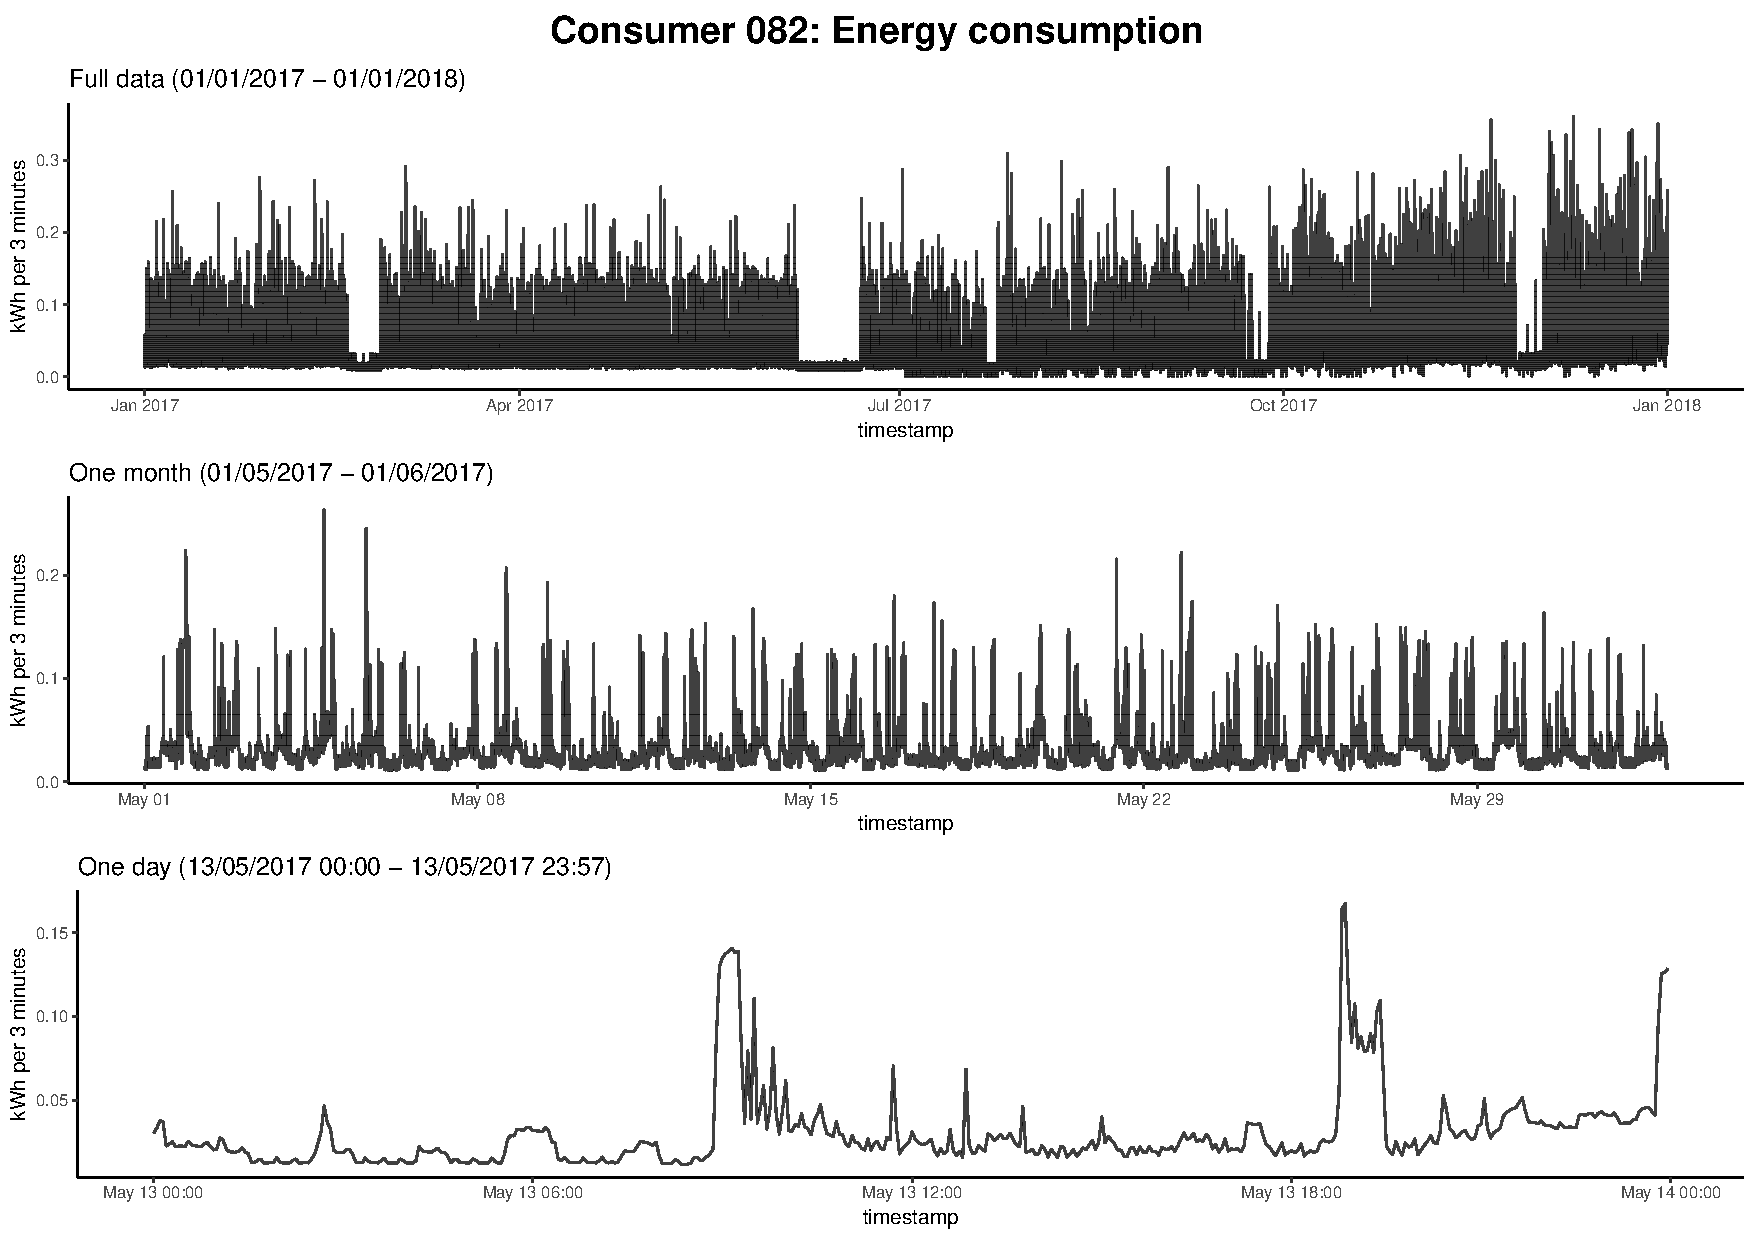
\includegraphics[width=\textwidth]{thesis/graphs/timeseries/c082_cons.pdf}
\caption[Energy consumption recordings of consumer 082]{Energy consumption recordings of consumer 082. The first panel shows the full year 2017, the second panel zooms in to one month (May), and the third panel zooms in to one day (May, 13). \quantnet}
\label{Fig:energycons_c082}
\end{figure}

Notably, there are two extended (in March and June) and three shorter periods (in July, September, and December) of clearly distinguishable low consumption and low fluctuation levels. The most likely explanations for these low, stable energy consumption periods are holidays, in which the household members are on vacation and leave appliances that are on standby or always turned on as the only energy consumers. This exemplifies the fact, that household members' behaviour is the biggest driver of fluctuations in the energy consumption of a household and the almost only cause for uncertainty in the time series.

Interestingly, the consumption time series of consumer 082 shows an increase in mean consumption starting with October 2017. This could be explained by colder outside temperatures. However, within the first quarter of 2017, no equivalent decrease in the mean energy consumption can be seen. Therefore, the reason for this increase might be given by newly acquired household appliances which are increasingly used with the approaching winter as the household members spend more time indoors.

The second panel zooms to just one month making daily fluctuation patterns already visible. In May there seem to be no abnormal consumption patterns. There are a few peaks in the first and third week of May that stand out, but no longer periods of very low energy consumption. More interestingly seems to be the last panel, which zooms in to just one day of energy consumption, i.e. May 13, 2017. This day was chosen for no particular reason other than that it is more or less in the middle of the month shown in the second panel. May 13, however, nicely exemplifies a usual pattern of energy consumption: There is low and rather stable energy consumption from midnight until about 7.30 a.m. which only fluctuates in a systematic and repeated way. Most probably, this "base consumption" is caused by appliances in standby and "always on" appliances, such as a fridge and/or freezer. At around 7.30 a.m., the household members probably wake up and the energy consumption spikes for the next 30 minutes -- the light is turned on, coffee is made, the stove is turned on, and maybe a flow heater is used to shower with hot water. As the household members leave the house (May 13 is a Monday), the consumption slowly decreases again. In the evening at about 6.30 p.m. energy consumption spikes again, probably caused by dinner preparations (and the usage of a microwave or stove). Not intuitively explainable, however, is the spike which is visible just before midnight. This spike, again, highlights the extreme uncertainty contained in individual household energy consumption. It is mostly caused by human behavior, which can seem quite erratic by just looking at energy consumption patterns without context.

To get a better impression of the representativity of consumer 082's energy consumption, it is compared to the other data sets available for this study. Figure \ref{Fig:cons_total_consumption} shows the total energy consumption 2017 in kWh of all consumers. As can be seen, consumer 082 (labelled c082 in Figure \ref{Fig:cons_total_consumption}) is at the lower end of the top quartile of the total energy consumption distribution across all consumers. The household's total energy consumption in 2017 was 6752.763 kWh. According to \citet{Stromspiegel:2017}, this number corresponds to a category D five-person household (on a scale from A (very low) to G (very high energy consumption)) that is heating its water with electricity. That means, the household of consumer 082 is either very big or has a comparatively very high energy consumption. Consumer 067, on the contrary, is remarkable as total consumption here is with only 40 kWh quite close to zero. At the high end of total consumption is consumers 025 with almost five times the total consumption of the average consumer in this data sets. Summary statistics for the total energy consumption of consumer households in 2017 can be found in Appendix \ref{App:Tables:totalcons}.

\begin{figure}[htbp]
 \centering
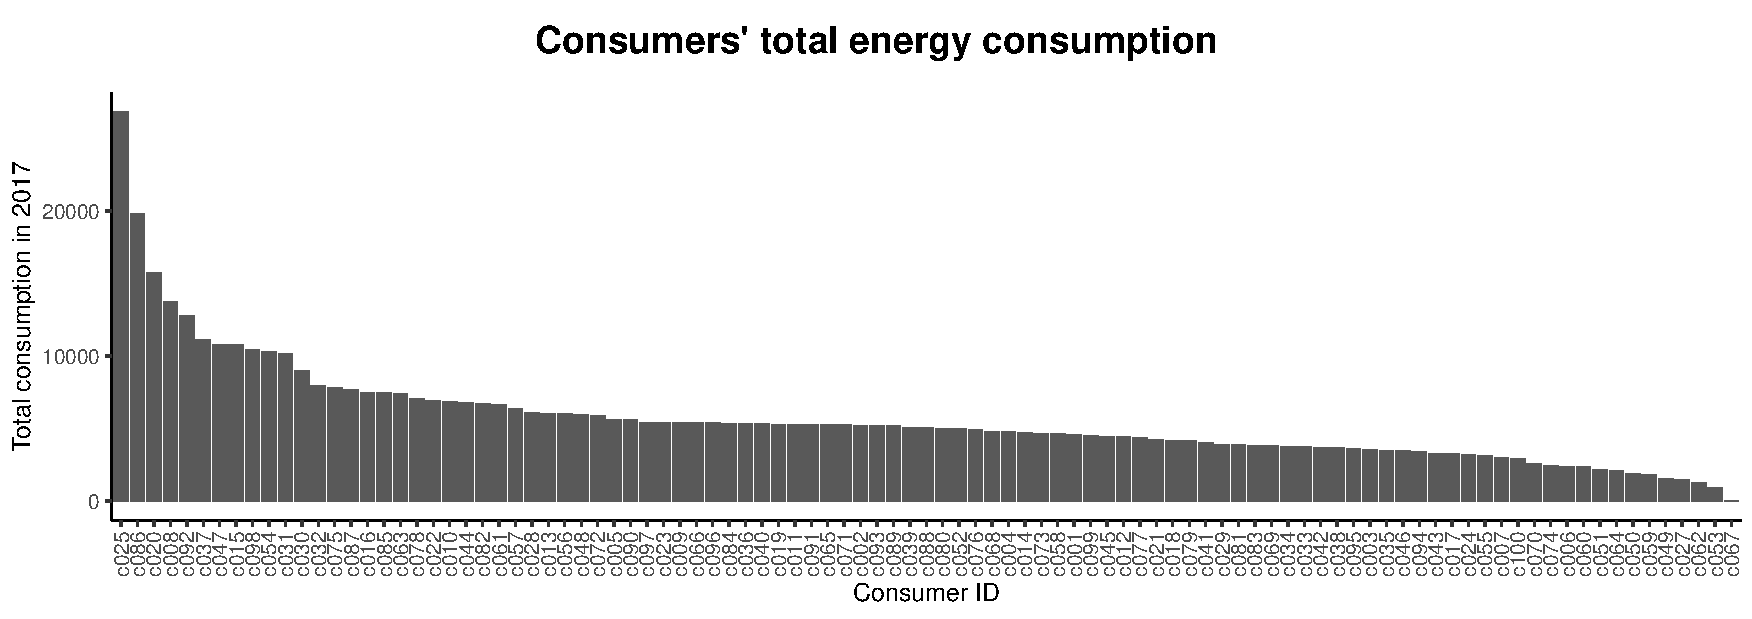
\includegraphics[width=\textwidth]{thesis/graphs/consumer_totalconsumption2.pdf}
\caption[Consumers' total energy consumption (in kWh) in 2017]{Consumers' total energy consumption (in kWh) in 2017 ordered from high to low. \quantnet}
\label{Fig:cons_total_consumption}
\end{figure}

Figure \ref{Fig:cons_boxplots_consumption} offers another perspective on the consumers' energy consumption. The figure shows a boxplot for each consumer's distribution of energy consumption per 3-minute interval. That means, the median line in the boxplot of a consumer is the consumers median consumption per 3-minute interval, while the box encloses the interquartile range (IQR) of the 3-minute consumption values of this particular consumer. It is apparent, that the IQR is for almost all consumers relatively small compared to the total range of their consumption values. All points plotted above the boxplots' whiskers are consumption values greater than the third quartile plus 1.5 $\times$ IQR. This again shows that there is a substantial amount of extreme values -- for which the description "outlier" not necessarily fits as they obviously occur quite often -- which are, most likely, hard to predict with standard forecasting methods.

\begin{figure}[htbp]
 \centering
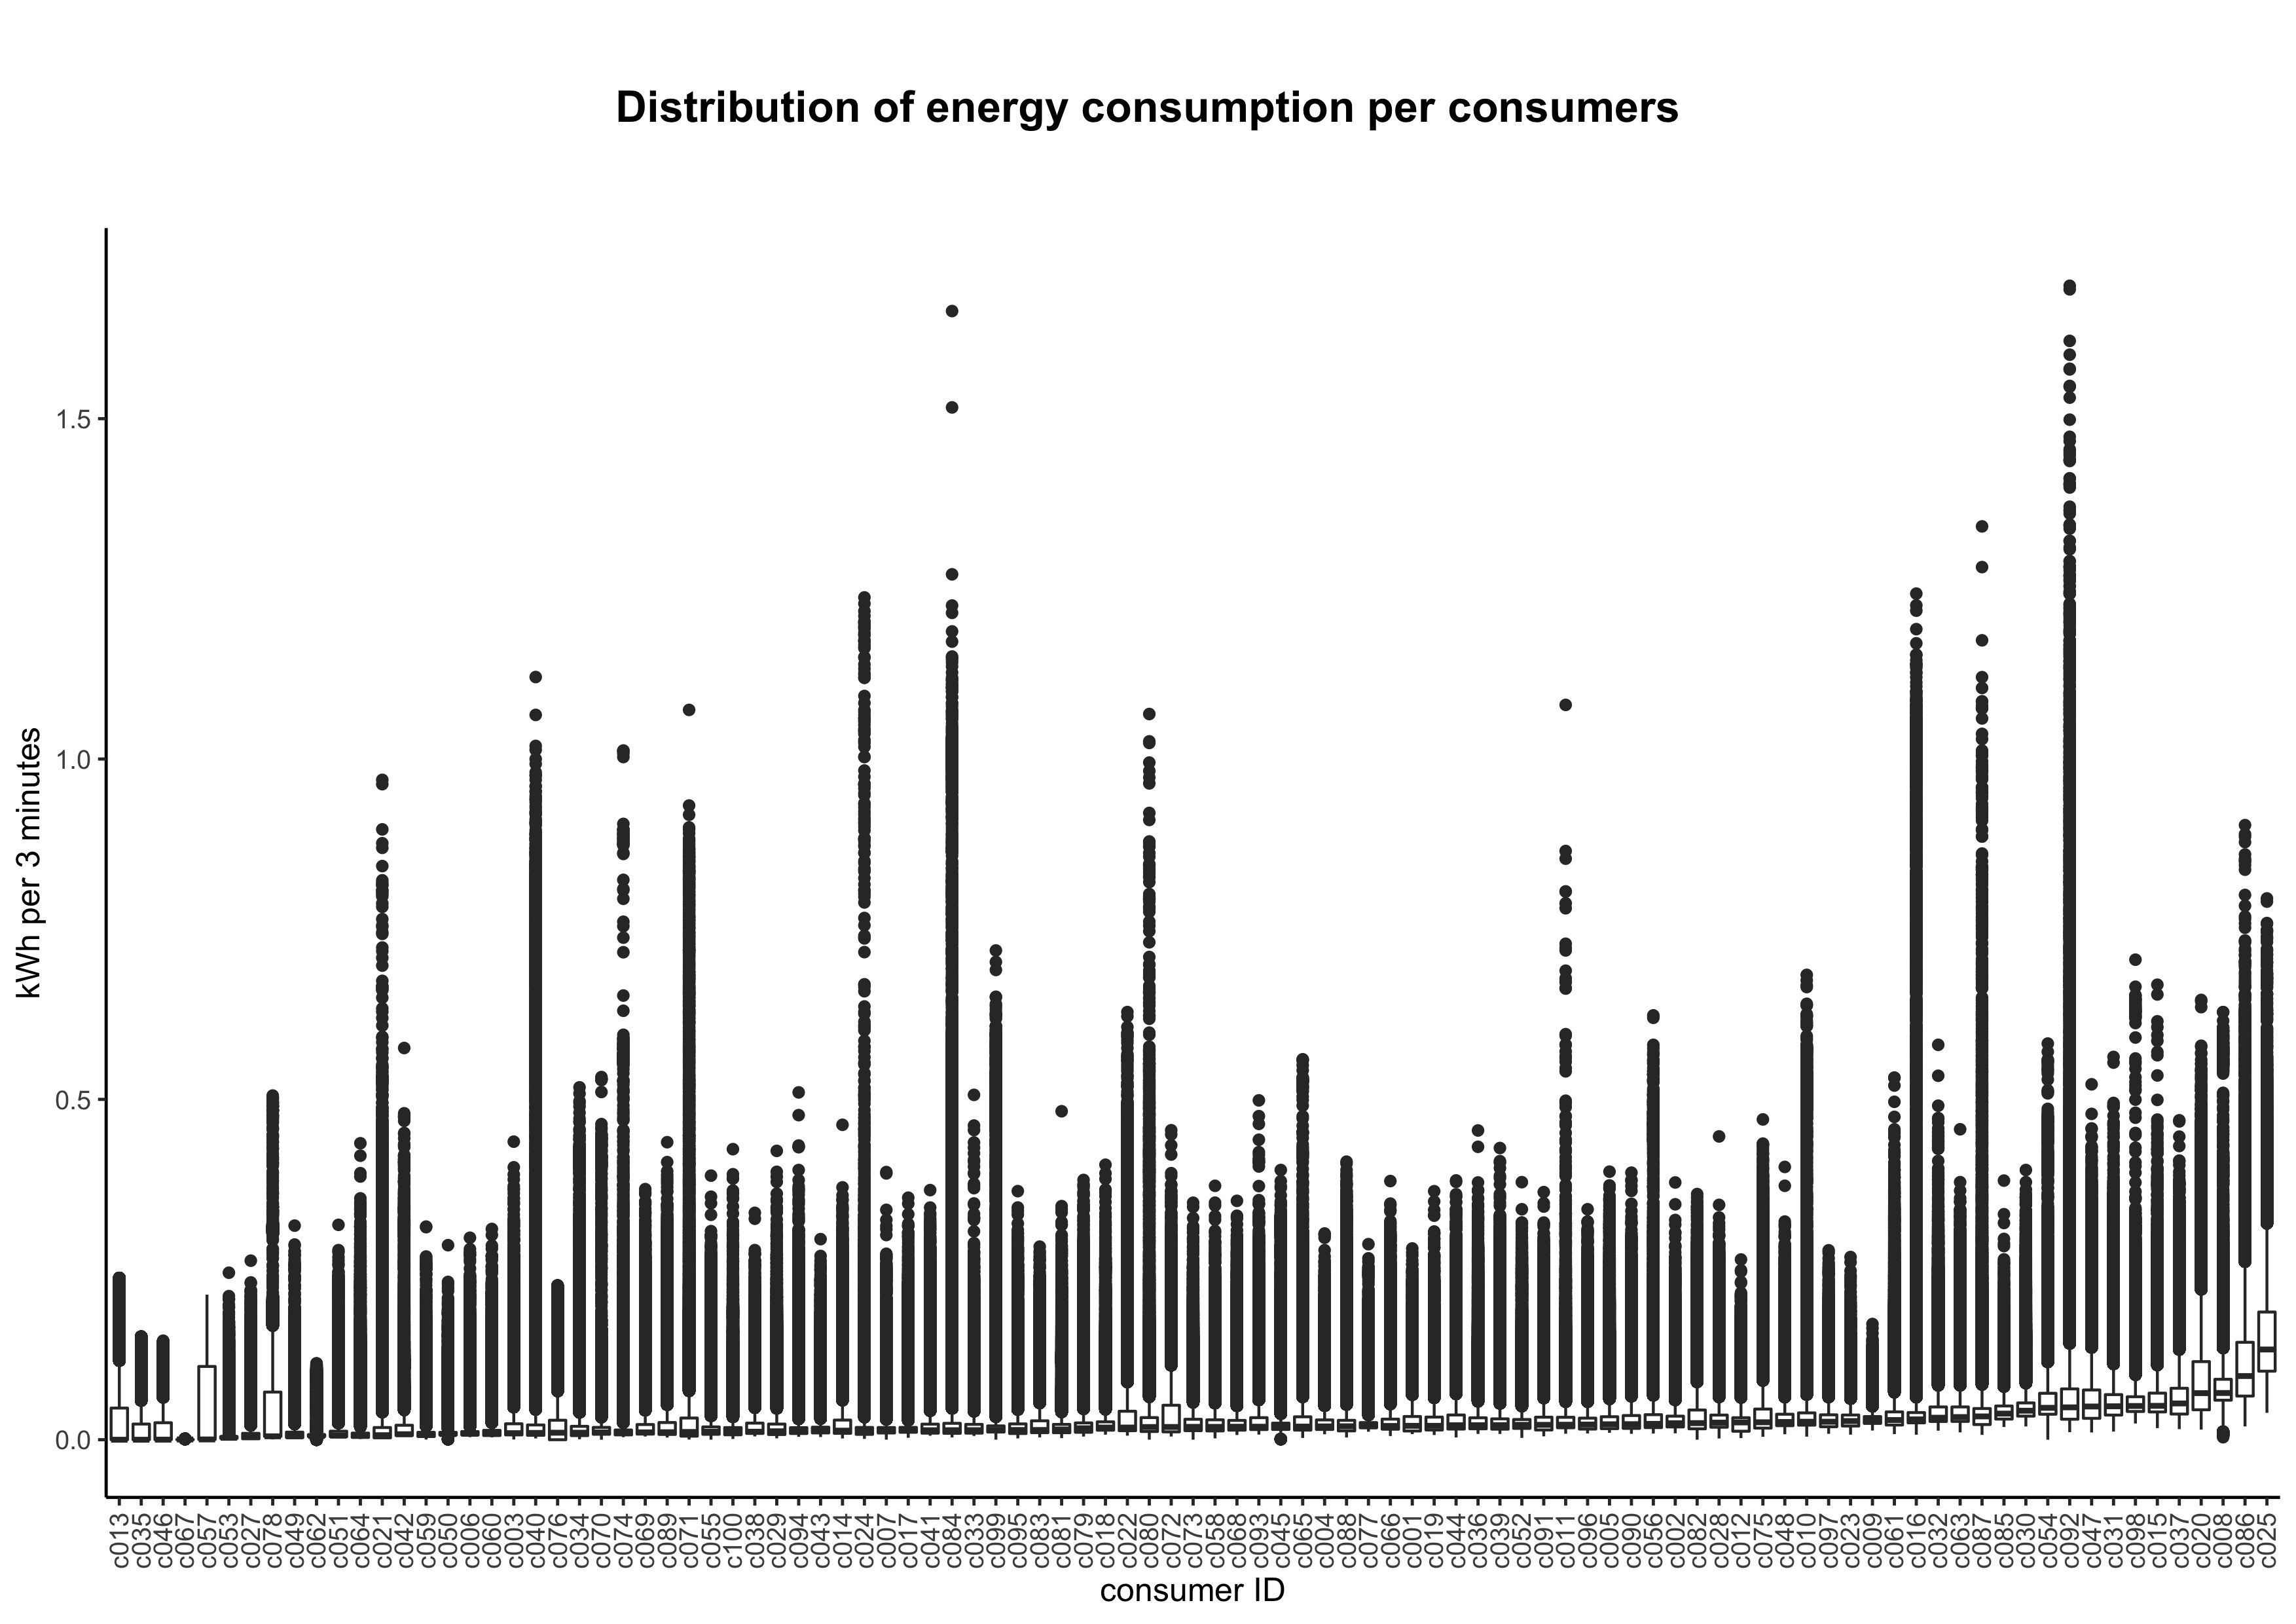
\includegraphics[width=\textwidth]{thesis/graphs/consumer_boxplots_consumption.jpg}
\caption[Boxplots of each consumer's energy consumption in kWh per 3-minute interval]{Boxplots of each consumer's energy consumption in kWh per 3-minute interval. \quantnet}
\label{Fig:cons_boxplots_consumption}
\end{figure}

%%%%%%%%%%%
\subsubsection{Prosumer data sets}

As it turns out, the prosumer data sets show very different consumption patterns than pure consumers. This may be due to the fact, that the recorded energy consumption per 3-minute interval is the net value of the actual energy consumption and the energy production in the same interval. For example, if prosumer 024's recorded consumption value is 0.021 kWh in the time period from 2017-05-13 06:03:00 to 06:06:00, and its energy production in the same interval is 0.018 kWh (which is not recorded and therefore not known), its actual energy consumption in that time interval is 0.039 kWh. However, this actual energy consumption is unknown as the energy production per 3-minute interval is not recorded. Only a surplus of energy production over consumption would be recorded as an increase in the energy out readings (see Table \ref{Tab:p089}) -- which is not the case in this example.

Visual inspection of the consumption time series of the prosumer data sets already reveals that the consumption patterns in most cases do not resemble the consumer households' consumption patterns. Generalized, four types of consumption patterns can be found in the prosumer data: (1) The net energy consumption of the prosumer is zero at night, starts to increase at around 6 a.m., fluctuates over daytime, and decreases to zero again at around 6 p.m. (see exemplary prosumer 004 in Figure \ref{Fig:prosenergycons_peculiar}). (2) The net energy consumption is mostly non-zero and fluctuates (in a regular pattern) at low levels with occasional net consumption spikes (see exemplary consumer 050 in Figure \ref{Fig:prosenergycons_peculiar}). This is the most generic type of prosumer energy consumption patterns. (3) The net consumption is for most of the year zero (see exemplary prosumer 061 in Figure \ref{Fig:prosenergycons_peculiar}). This may be due to a surplus in net energy production. (4) The net energy consumption is mostly non-zero and fluctuates very little at a relatively high level (see exemplary prosumer 093 in Figure \ref{Fig:prosenergycons_peculiar}). The net energy consumption drops only occasional from this high level. Type (1) and (2) represent the majority of data sets. Type (1) is very easily identifiable and represents 30 \% of the data sets. Type (2) is more generic and therefore comprises more heterogenic patterns with 56 \% of the data sets belonging to this type. Type (3) and (4), exemplary shown in the lower two panels of Figure \ref{Fig:prosenergycons_peculiar}, only represent a minority of the data sets.

\begin{sidewaysfigure}[htbp]
    \centering
    \begin{minipage}[h]{\dimexpr.5\textheight-0.15em}
    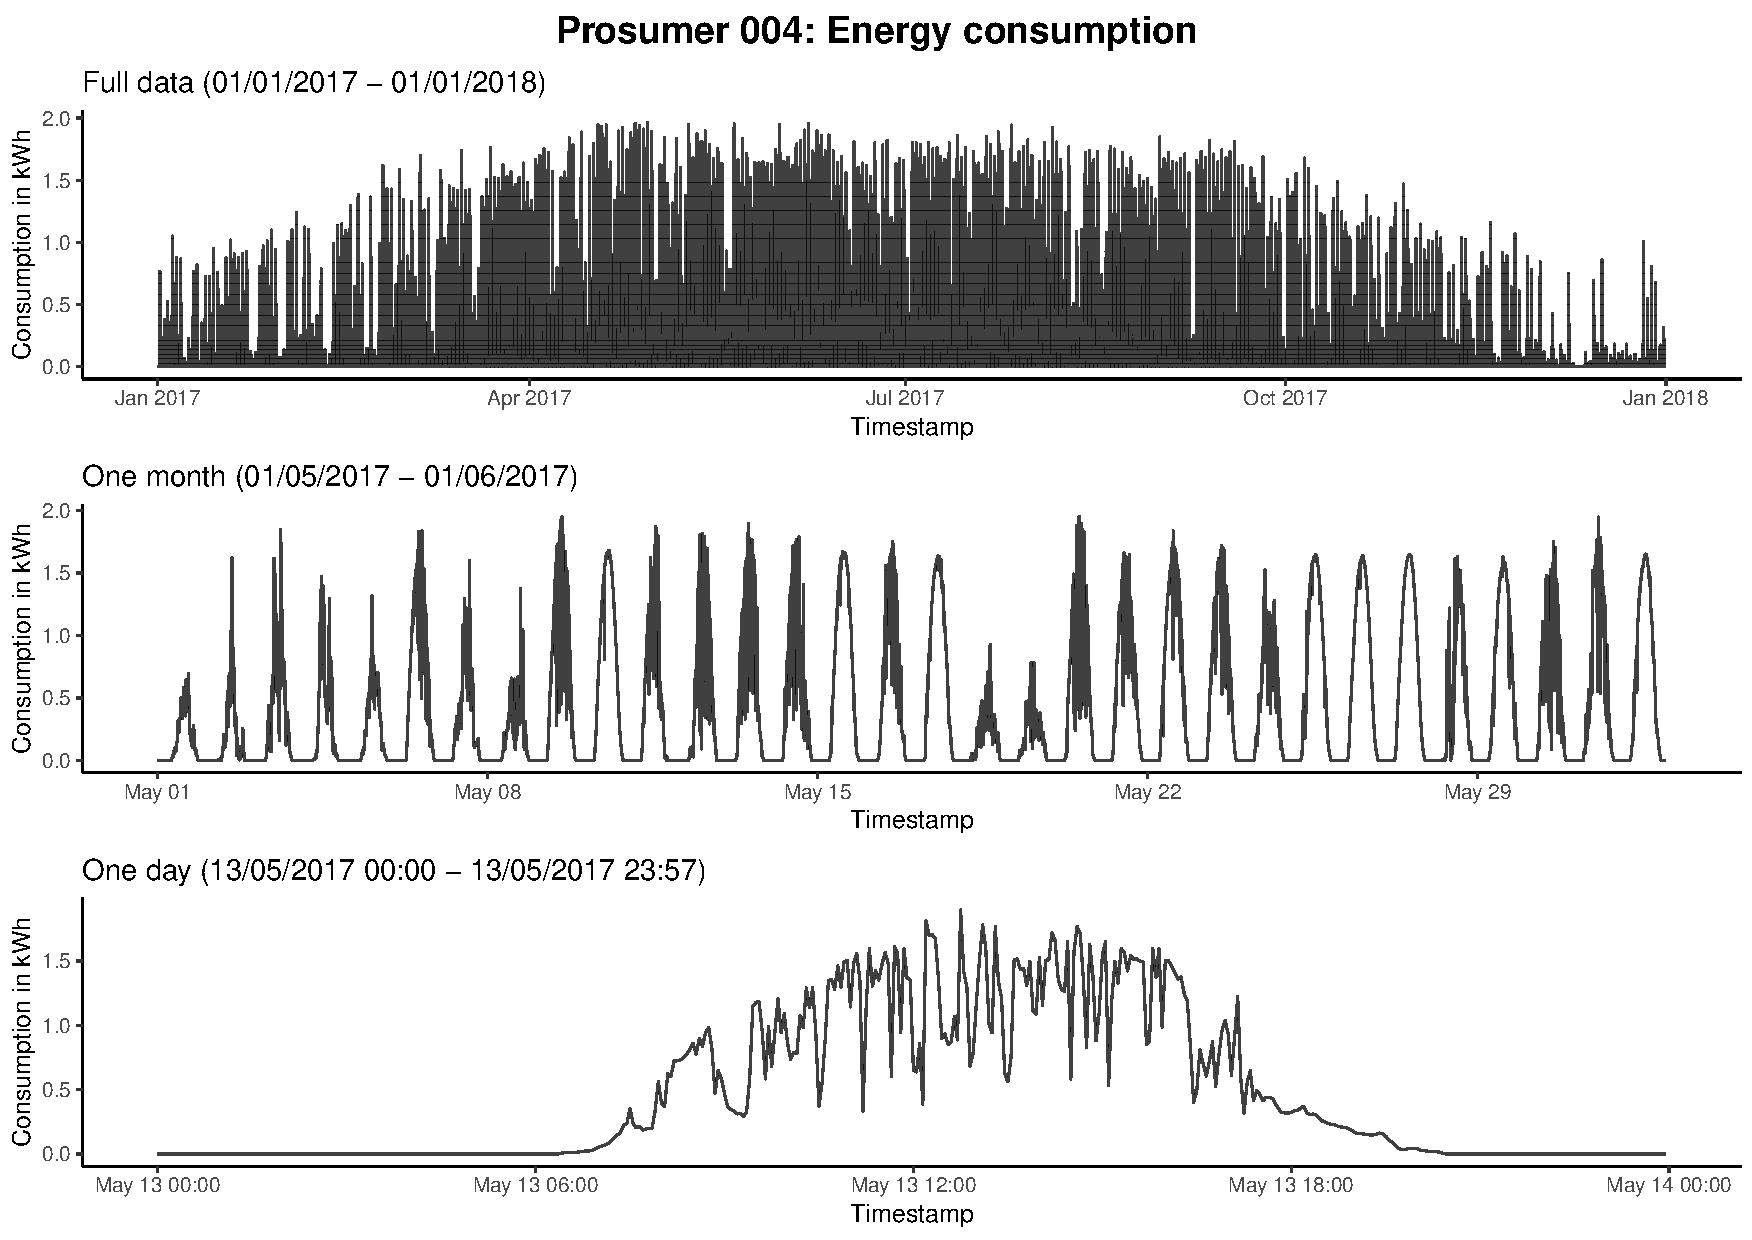
\includegraphics[width=\textwidth]{thesis/graphs/timeseries/p004_cons.pdf}
    \end{minipage}
    \begin{minipage}[h]{\dimexpr.5\textheight-0.15em}
    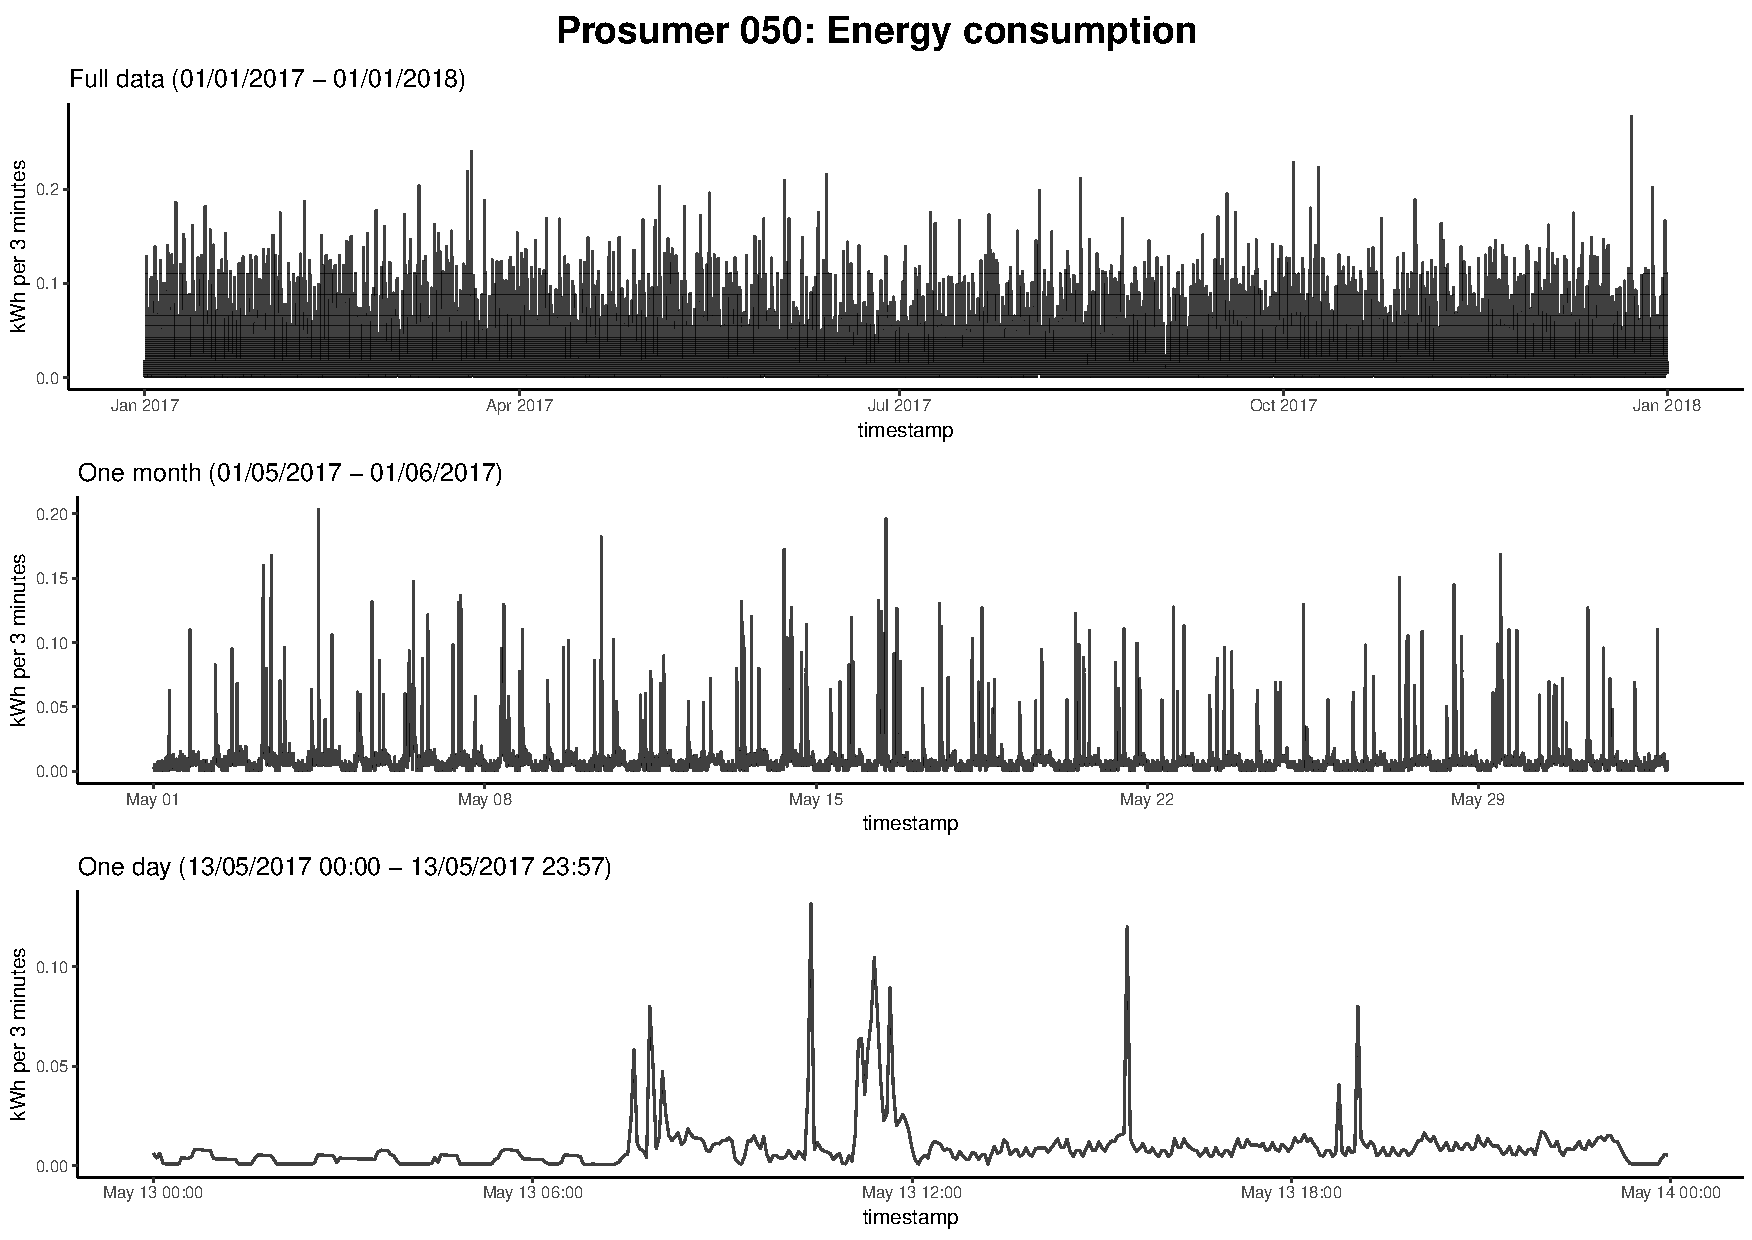
\includegraphics[width=\textwidth]{thesis/graphs/timeseries/p050_cons.pdf}
    \end{minipage}\\
    
    \begin{minipage}[h]{\dimexpr.5\textheight-0.15em}
    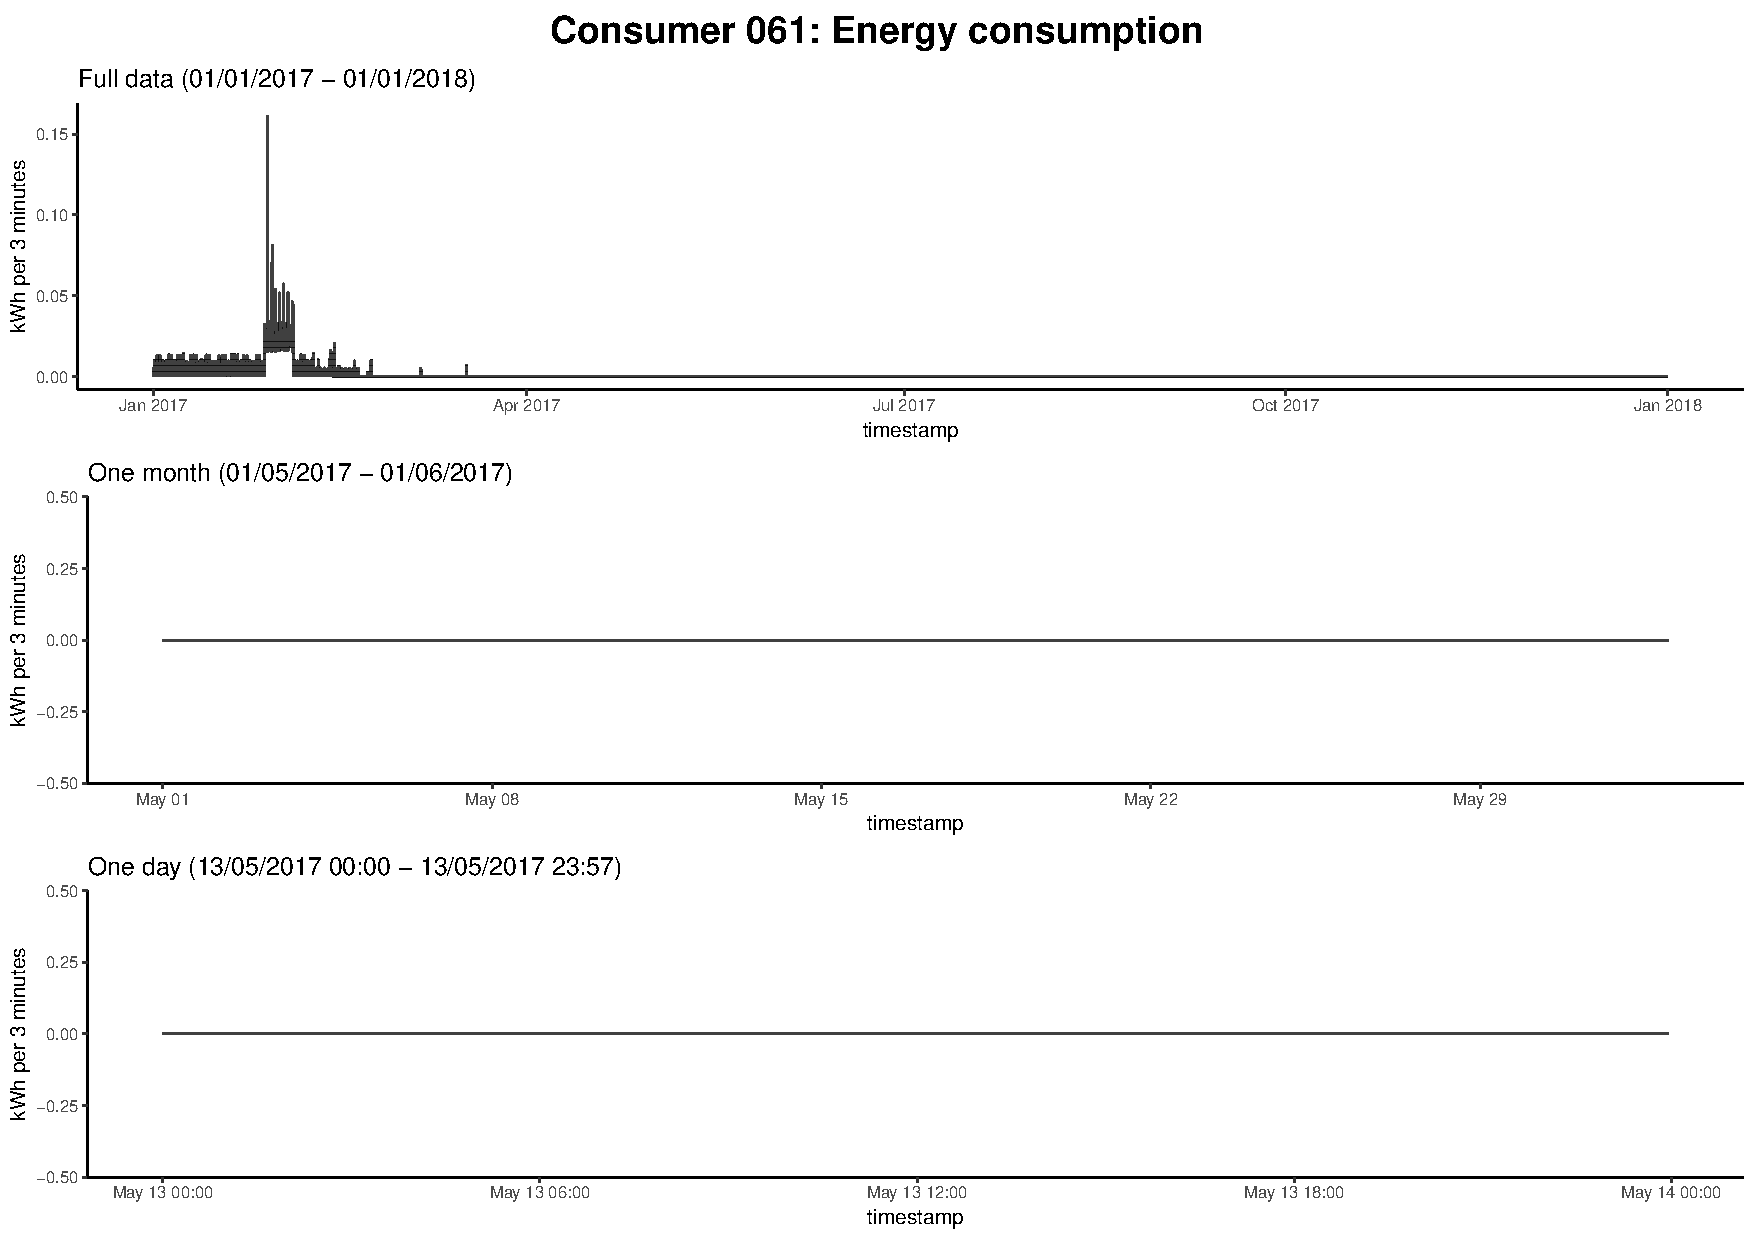
\includegraphics[width=\textwidth]{thesis/graphs/timeseries/p061_cons.pdf}
    \end{minipage}
    \begin{minipage}[h]{\dimexpr.5\textheight-0.15em}
    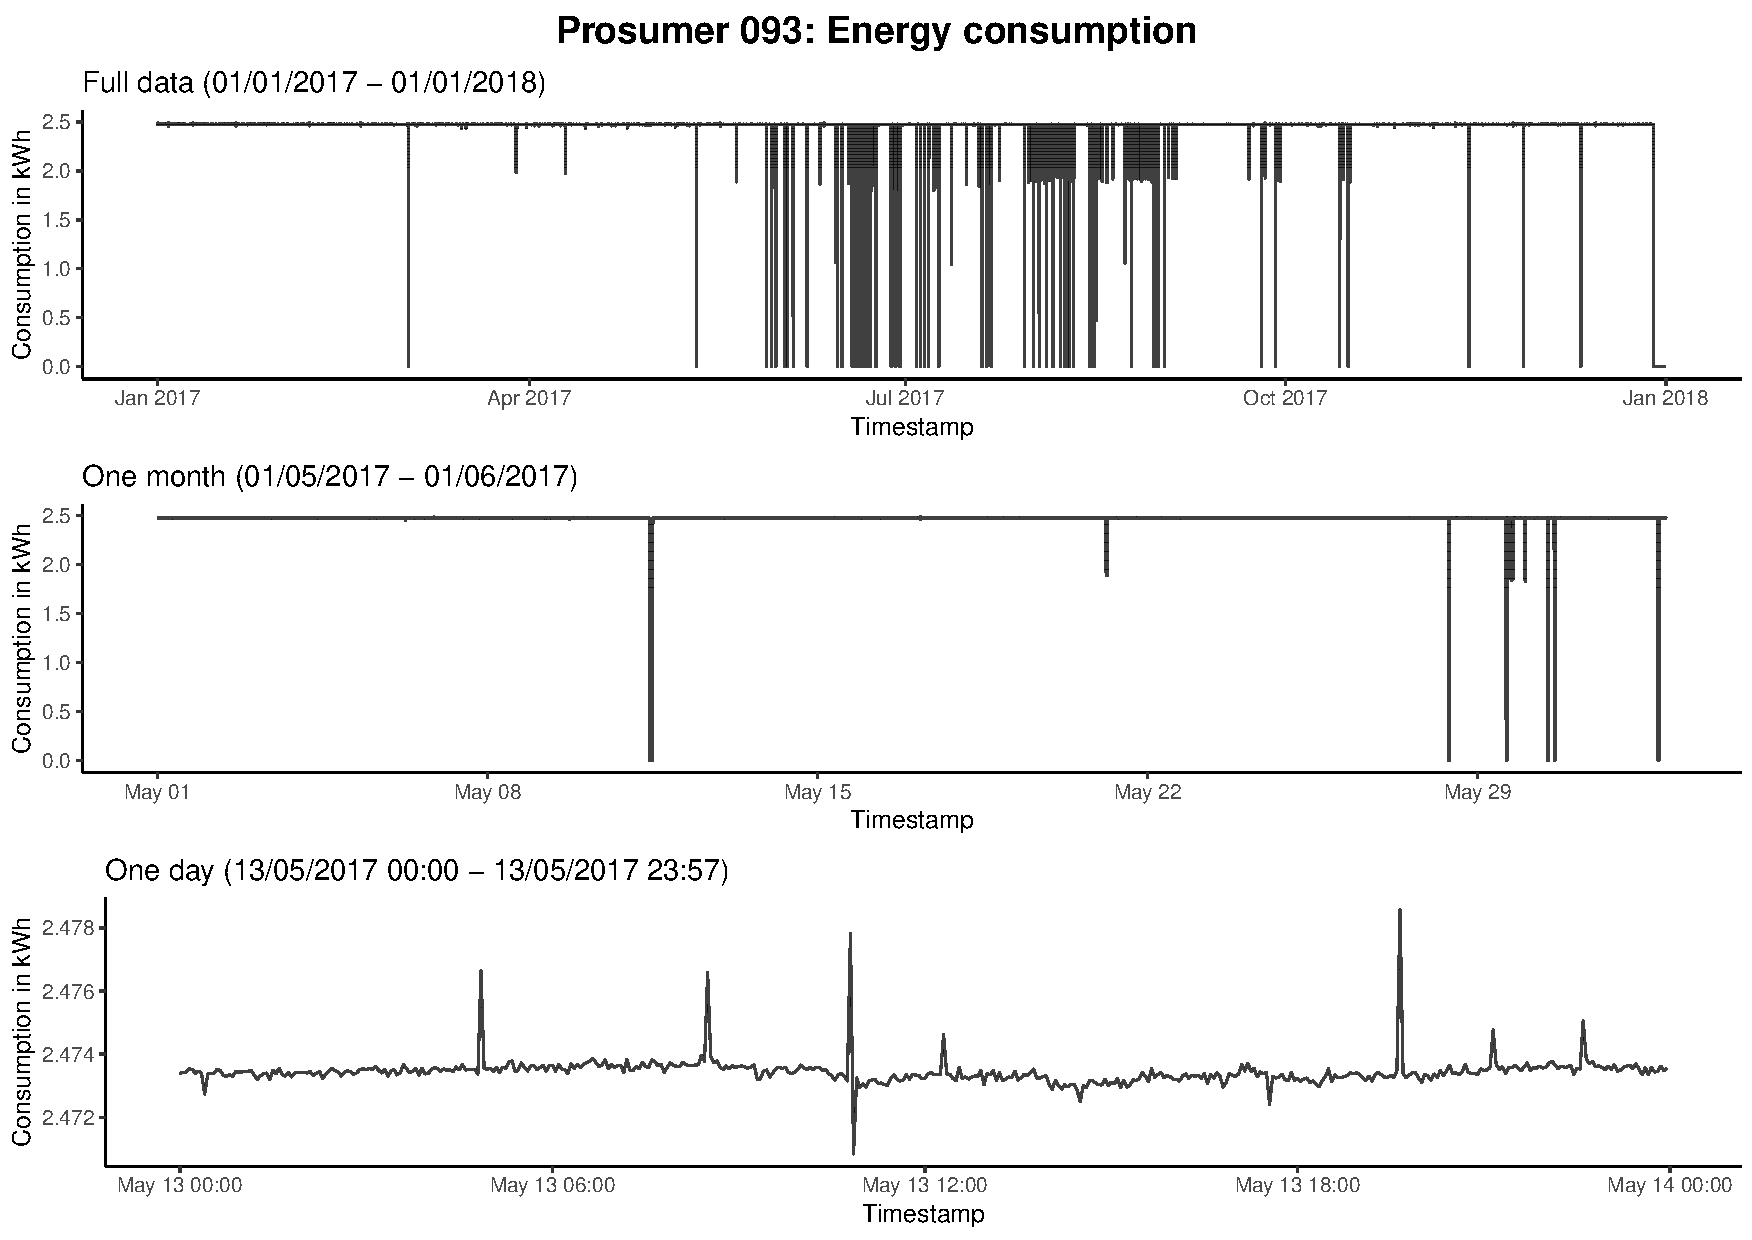
\includegraphics[width=\textwidth]{thesis/graphs/timeseries/p093_cons.pdf}
    \end{minipage}
    
    \caption[Different types of prosumer energy consumption patterns]{Different types of prosumer energy consumption patterns. \quantnet}
    \label{Fig:prosenergycons_peculiar}
\end{sidewaysfigure}

In conclusion, it becomes clear that the net energy consumption of prosumers may exhibit very different patterns than the energy consumption of consumers. This exacerbates the prediction task for prosumers significantly.

Furthermore, the total consumption of prosumers follows a very different distribution than the total consumption of consumers. The maximum total net consumption of a prosumer was 424,893.434 kWh, which is by a factor of 15 more than the maximum total net consumption of a prosumer. 19 out of 100 prosumers net consumed more energy than the biggest consumer household contained in the data. Also, the dispersion of the total net consumption is much higher with an IQR of 22,149 kWh for prosumers' total net consumption compared to an IQR of 2,542 kWh for consumers' total consumption in 2017.

\begin{figure}[htbp]
 \centering
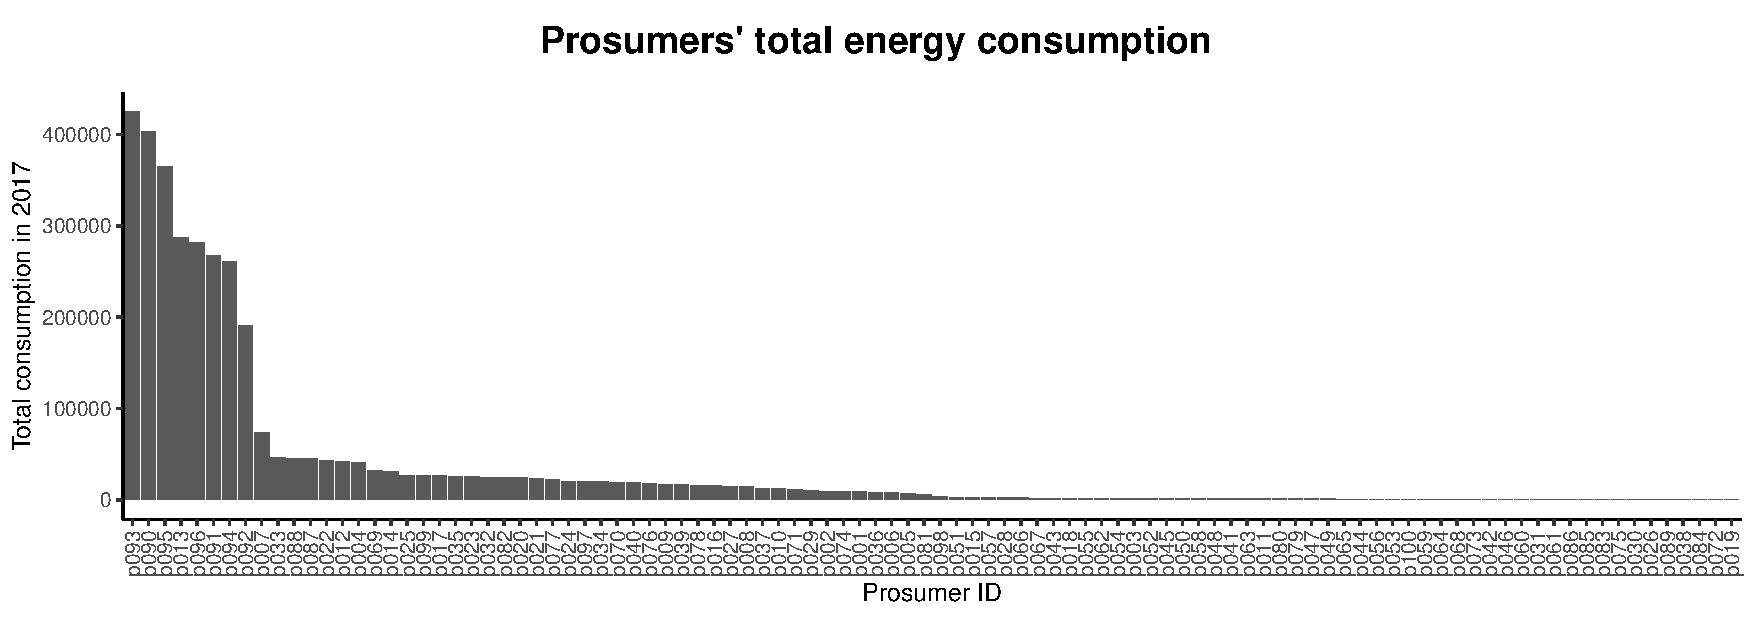
\includegraphics[width=\textwidth]{thesis/graphs/prosumer_totalconsumption2.pdf}
\caption[Prosumers’ total energy consumption (in kWh) in 2017]{Prosumers’ total energy consumption (in kWh) in 2017 ordered from high to low. \quantnet}
\label{Fig:pros_total_consumption}
\end{figure}

Finally, Figure \ref{Fig:pros_boxplots_consumption} offers another perspective on the heterogeneity of the prosumer data sets. The figure shows a boxplot for each prosumer's distribution of energy consumption per 3-minute interval. The prosumers are sorted on the x-Axis by their median net energy consumption. As can be seen, while the median for the majority of the prosumers is relatively close to zero, the IQR and the total range of net consumption values differs substantially between prosumers. Approximately the same range of net consumption values per 3-minute interval can be accompanied by a median of 0.0003 kWh (see p088 in Figure \ref{Fig:pros_boxplots_consumption}) or by a median of 1.9110 kWh (see p094 in Figure \ref{Fig:pros_boxplots_consumption}).

\begin{figure}[htbp]
 \centering
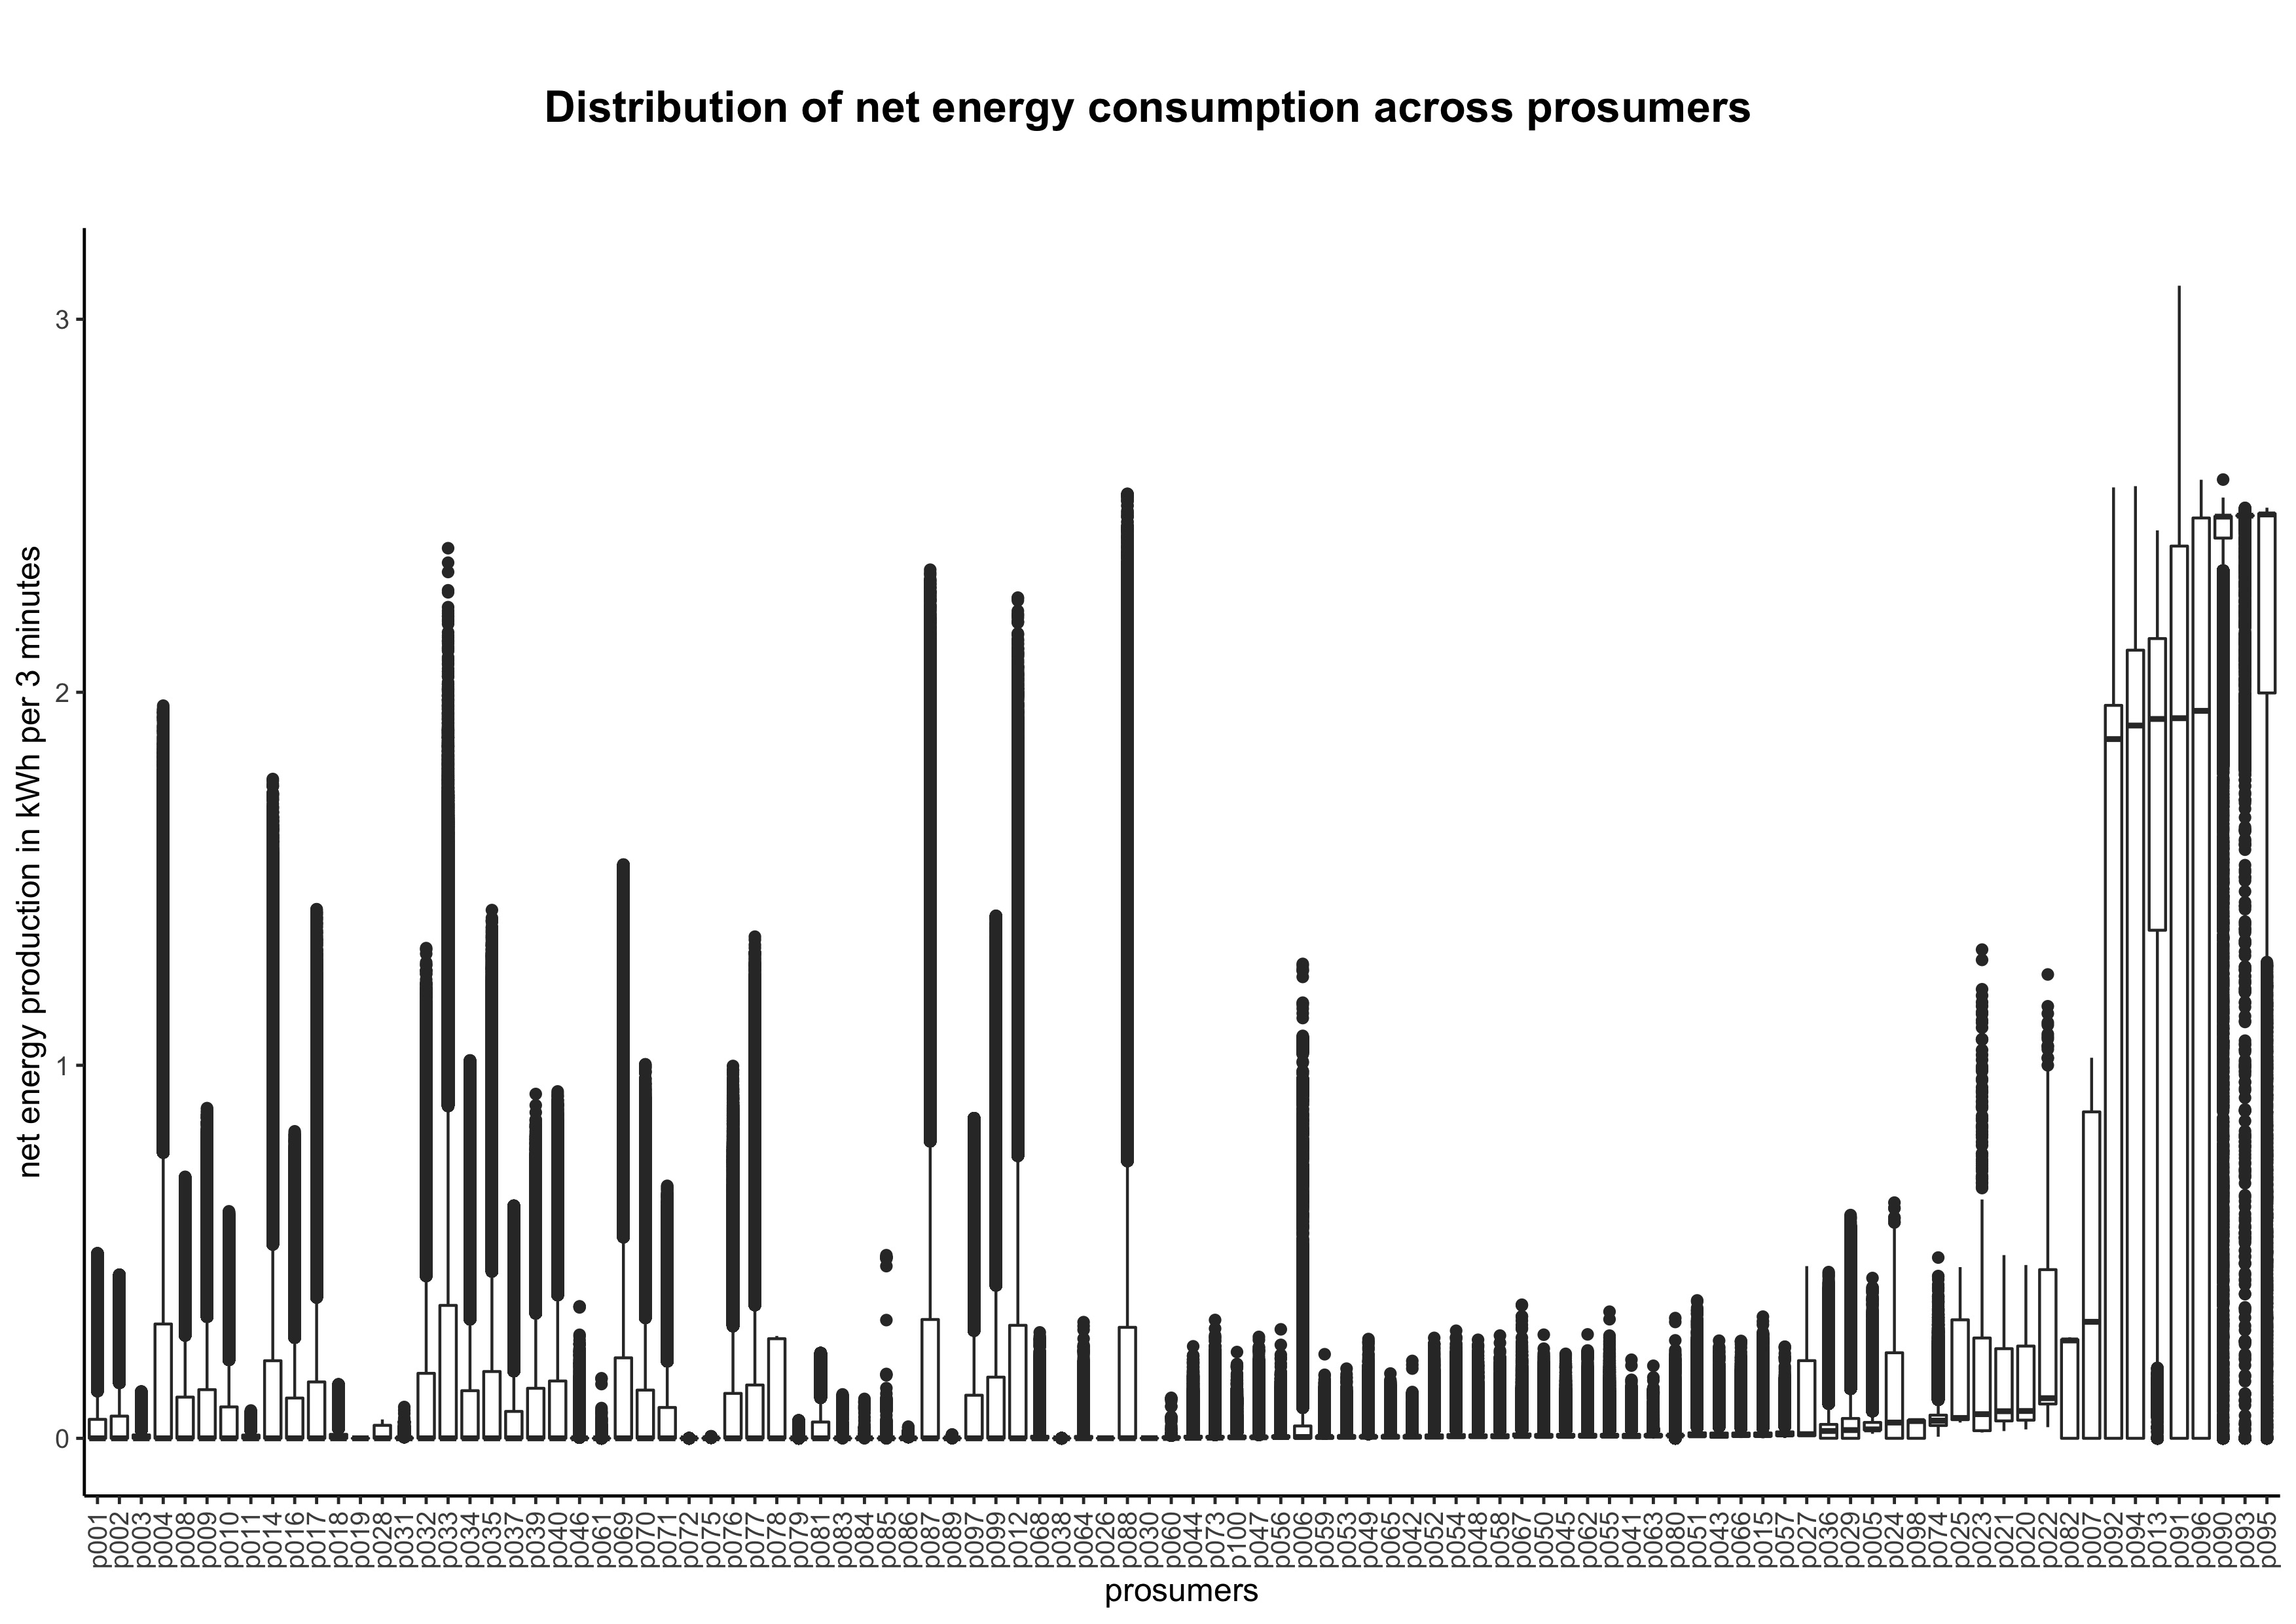
\includegraphics[width=\textwidth]{thesis/graphs/prosumer_boxplots_consumption.jpg}
\caption[Boxplots of each prosumer's net energy consumption in kWh per 3-minute interval]{Boxplots of each prosumer's net energy consumption in kWh per 3-minute interval. \quantnet}
\label{Fig:pros_boxplots_consumption}
\end{figure}

Prosumers are defined by the fact, that they not only consume energy but also produce energy -- primarily for their own consumption. However, any surplus in energy production over energy consumption is fed into the grid and, thus, recorded by the smart meter as an increase in the energy out readings. As explained above, these energy out readings are used to compute the net energy production per 3-minute interval by first-differencing. Surprisingly, only 14 out of 100 available prosumer data sets contained non-zero net energy production values at all. This becomes clear when looking at Figure \ref{Fig:pros_total_production}, which shows the total net energy production of all prosumers. 86 of those prosumers fed zero kWh into the grid during 2017. The top three net energy producing prosumers, however, fed a total of 1,259,686 kWh into the grid, which is more than twice the amount all 100 consumer households consumed together\footnote{Cumulatively, the 100 consumer households, for which data is available, consumed 559,369 kWh in 2017}. For comparison, a typical photovoltaic (PV) installation on a private residential building with a roof surface area of 150 m$^2$ produces approximately 20,000 kWh per year \citep{energieatlas:2018}.

\begin{figure}[htbp]
 \centering
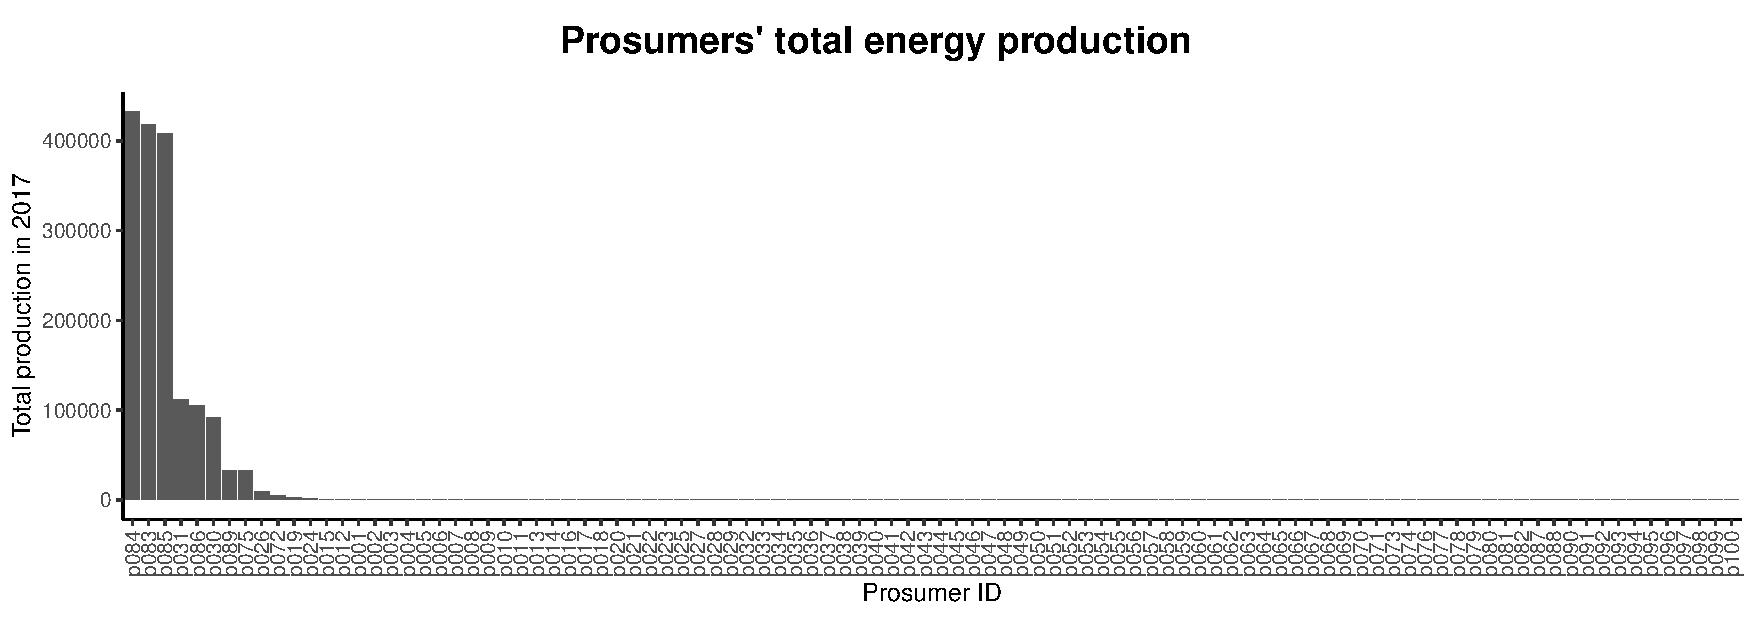
\includegraphics[width=\textwidth]{thesis/graphs/prosumer_totalproduction2.pdf}
\caption[Prosumers’ total energy production (in kWh) in 2017]{Prosumers’ total energy production (in kWh) in 2017 ordered from high to low. \quantnet}
\label{Fig:pros_total_production}
\end{figure}

Prosumer 026, for example, has a relatively low total net energy production. However, its net energy production pattern looks like a typical household with a PV installation (see Figure \ref{Fig:energyconsprod_p026p086}). The net energy consumption is (almost) always zero, while the net energy production on most days rather smoothly increases and decreases throughout the day with occasional drops, probably caused by changes in the cloud cover. Furthermore, the net energy production increases in the summer months and decreases notably in winter.

Compare this to prosumer 086 that has a stable, very high net energy production over the whole course of 2017. There are only few drops, which are accompanied by a simultaneous net energy consumption (visible by the small blue spikes in the upper panel of the right graph of Figure \ref{Fig:energyconsprod_p026p086}, whenever the net production drops). Note also the different scales of the y-axis. The net production of prosumer 084 plays in the range of 1 kWh per 3-minute interval while the net production of prosumer 026 barely surpasses 0.4 kWh per 3-minute interval. A plausible explanation for the kind of net production pattern exhibited by prosumer 086 may be a combined heat and power unit (CHP) (also known as block-type thermal power station (BTTP)). This is also indicated by the increasing frequency of drops in net energy production over the summer months. In these months much less heating is needed resulting in more downtime of the CHP and therefore also more periods of zero net energy production. However, as mentioned in the discussion of the consumer data sets, unfortunately, there is no additional context information available for the data sets at hand making this kind of assumption purely speculative.

\begin{sidewaysfigure}[htbp]
\centering
\begin{minipage}[h]{\dimexpr.5\textwidth-0.15em}
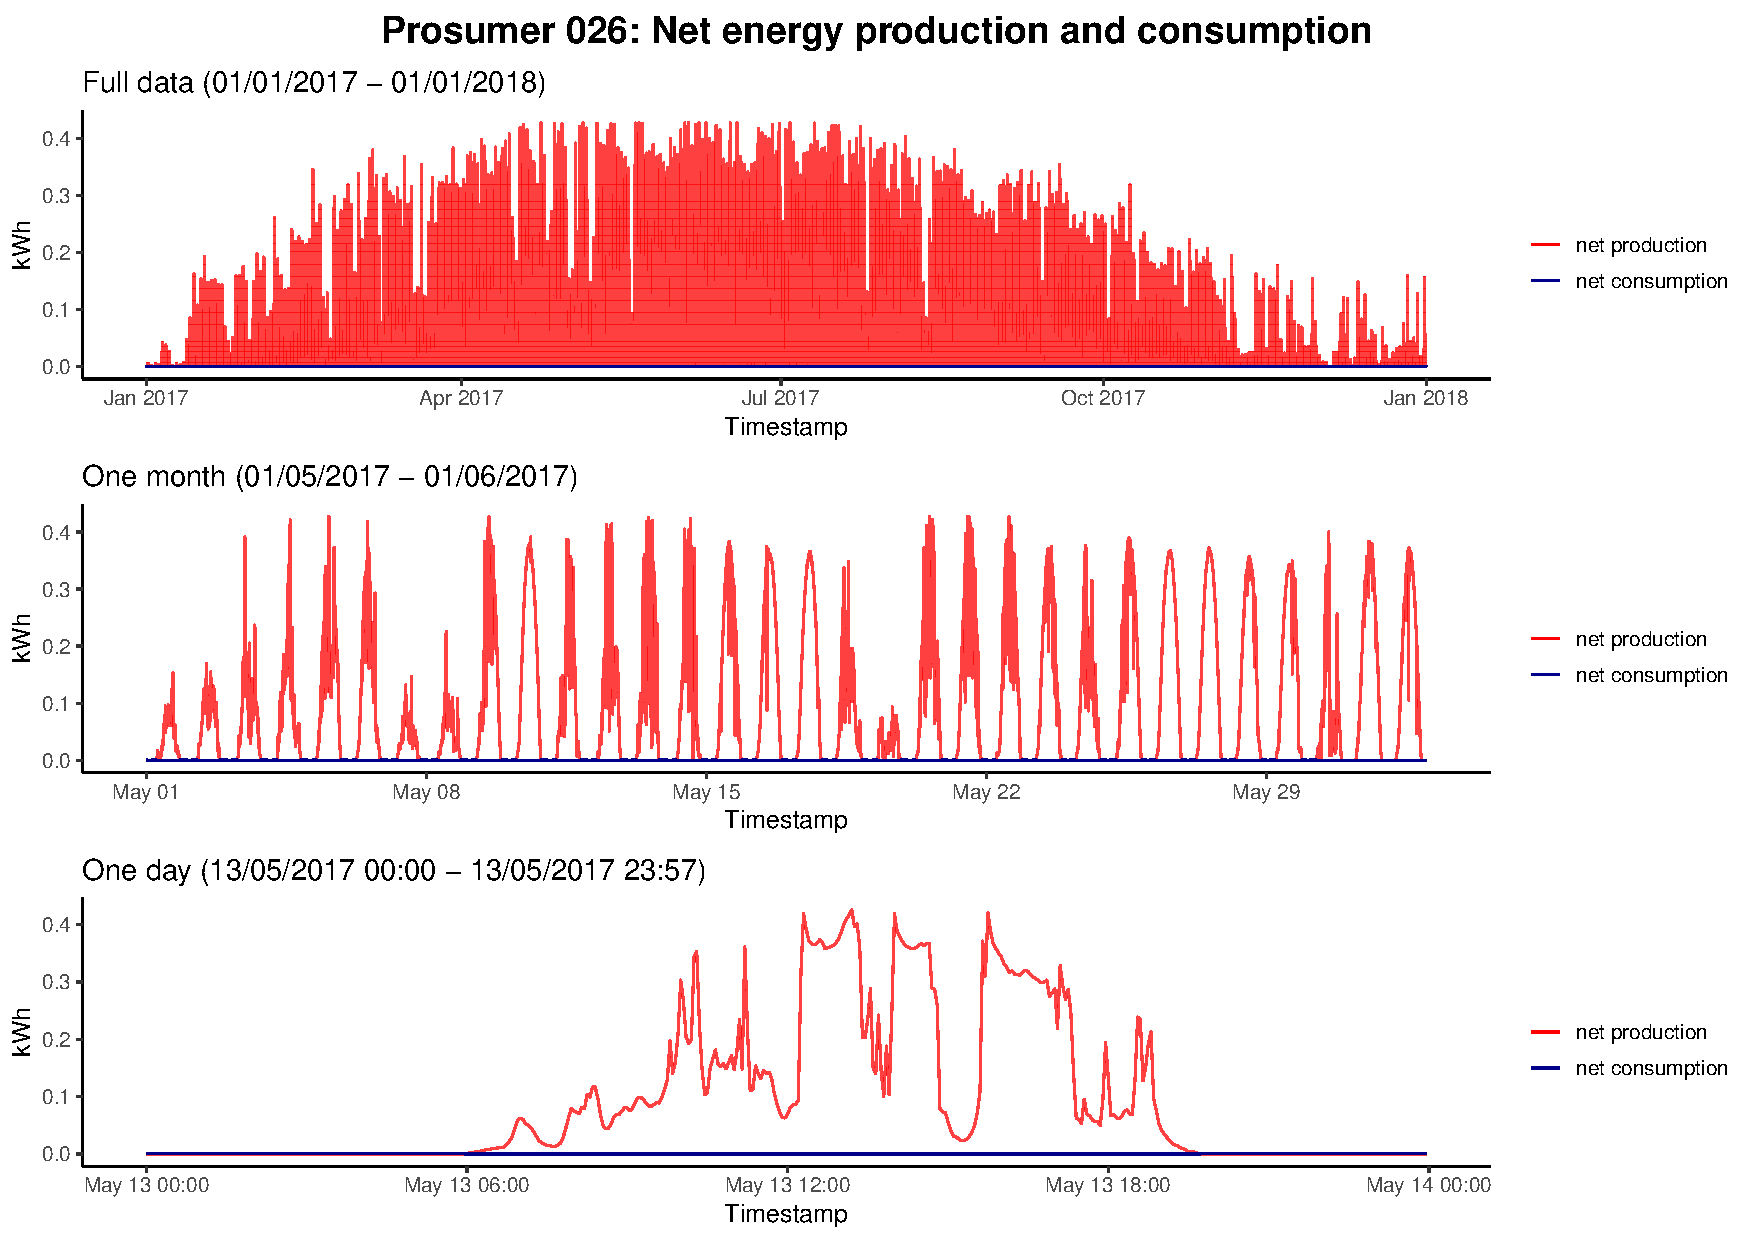
\includegraphics[width=\textwidth]{thesis/graphs/timeseries/p026_prod&cons.pdf}
\end{minipage}
\begin{minipage}[h]{\dimexpr.5\textheight-0.15em}
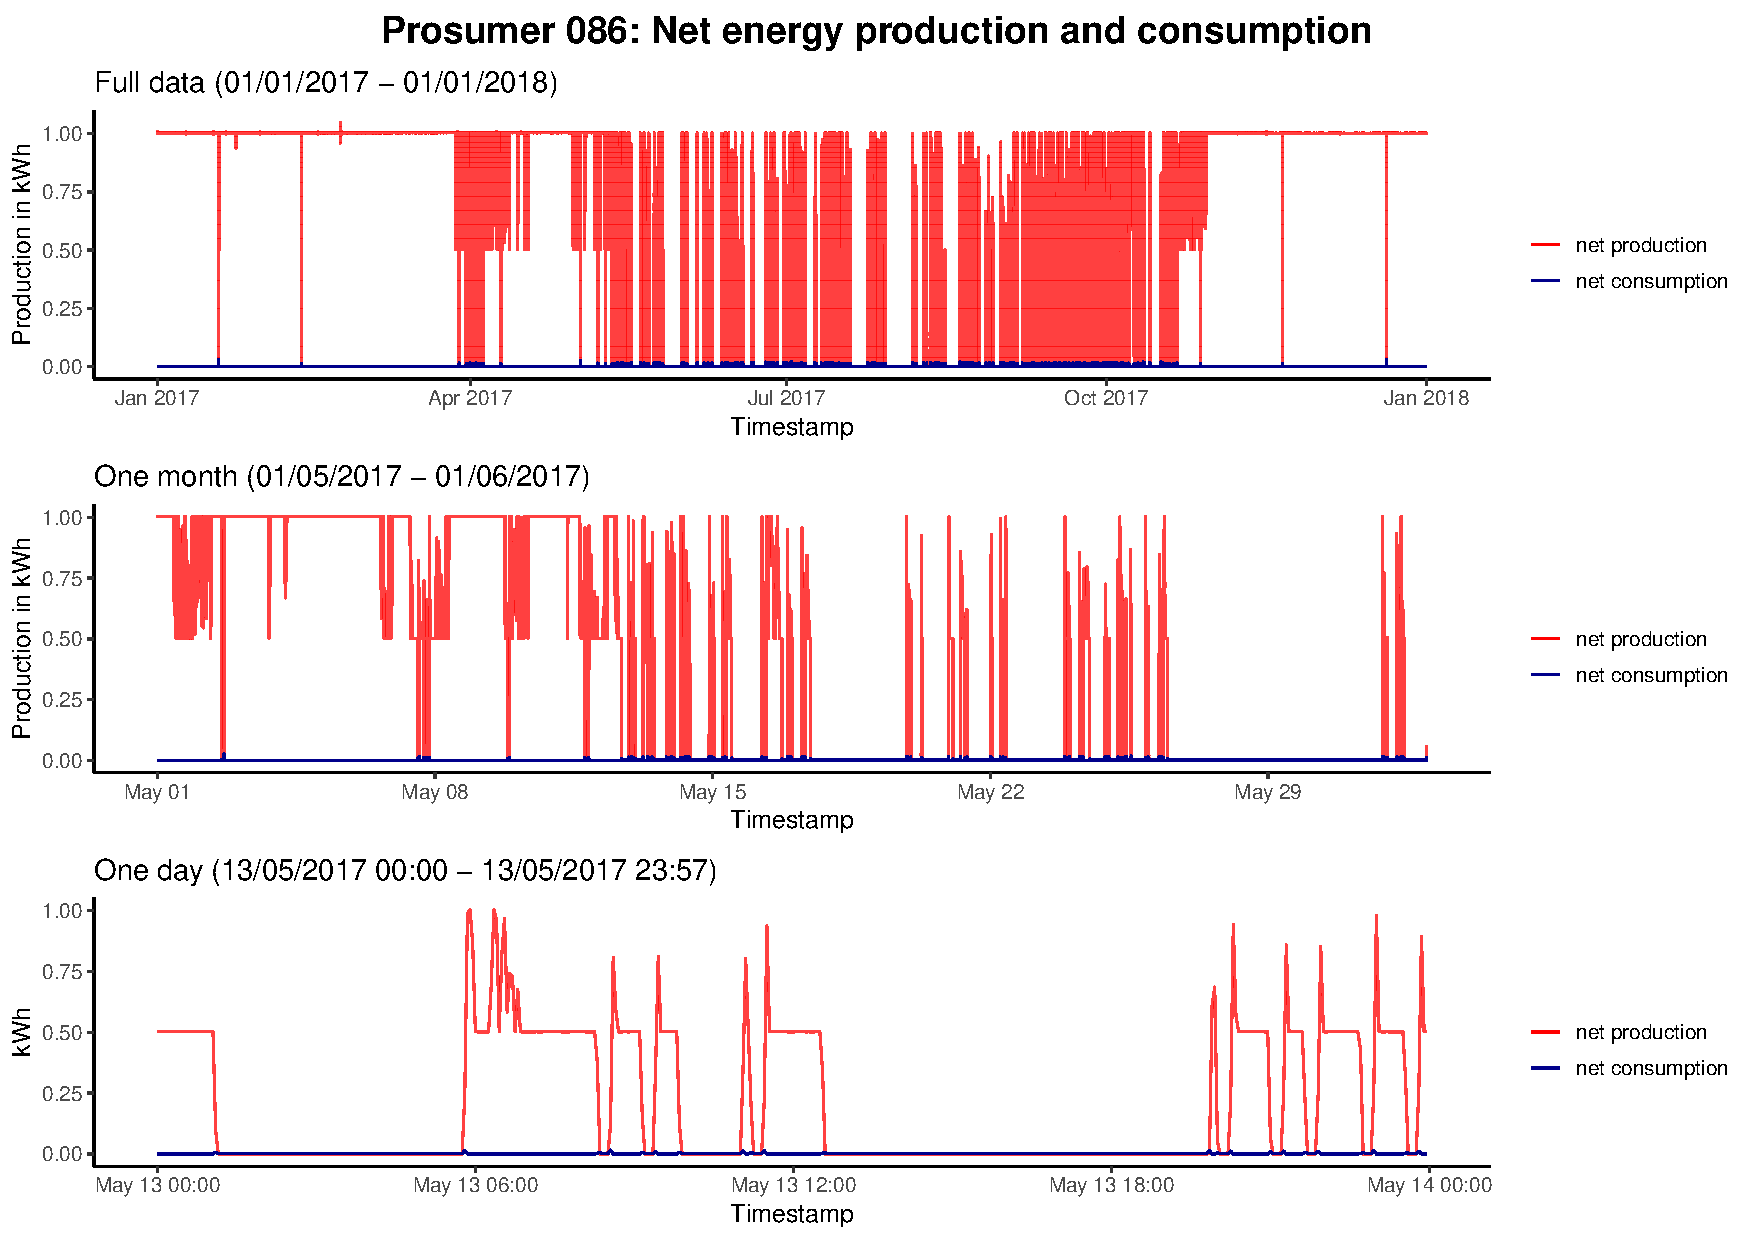
\includegraphics[width=\textwidth]{thesis/graphs/timeseries/p086_prod&cons.pdf}
\end{minipage}

\caption[Energy consumption and production recordings of prosumers 026 and 086]{Energy consumption and production recordings of prosumers 026 and 086. The first panel in the respective graph shows the full year 2017, the second panel zooms in to one month (May), and the third panel zooms in to one day (May, 13). \quantnet}
\label{Fig:energyconsprod_p026p086}

\end{sidewaysfigure}

In conclusion, it becomes clear that the prosumers' net energy consumption and production follow much less easily explained patterns. The net energy consumption is much more heterogeneous. Additionally, most prosumer data sets do not contain any recordings of net energy production at all. Of those prosumers that do have positive net production values, most surpass the energy consumption of a typical household with their net energy production by far. Implications of this for the suitability of the data sets for the prediction task at hand will be discussed in Section \ref{Sec:Data;Subsec:Exclusion}.

%%%%%%%%%%%%%%%%%%%%%%%%%%%%%%%%%%%%%
%%%   Peculiarities in the data   %%%
%%%%%%%%%%%%%%%%%%%%%%%%%%%%%%%%%%%%%

\subsection{Peculiarities in the data}\label{Sec:Data;Subsec:Peculiarities}

%%%%%%%%%%%
\subsubsection{Consumer data sets}

The data sets were analyzed for peculiarities in the time series patterns that seemed to be systematically different than the majority of data sets. One such peculiarity is the occurrence of zero values. In any household that does not produce its own energy (pure consumer household), energy consumption of 0 kWh, even only for a very short period of time, seems to be very unlikely (apart from the rare case of a power outage in the area or when the main switch of the household is turned off). Thus, it is not surprising that 93 \% of the data sets do not contain any 0 kWh measurements per 3-minute interval at all. Of the remaining 6 data sets, one contains just a single measurement of 0 kWh, which seems plausible. The other data set with a negligible amount of zero values is consumer 082 which was discussed in detail in section \ref{Sec:Data;Subsec:Description}. In Figure \ref{Fig:energycons_c082} showing consumer 082 consumption values, it is visible that although the consumption pattern does not change substantially, the lowest values of the daily fluctuations are lower in the second half of 2017 than in the first half. However, this seems still a plausible consumption pattern for a typical household. The other five data sets, on the contrary, contain between 34 and 54 \% of zero values. Examining the consumption time series more closely also reveals, that these households exhibit a systematically different consumption pattern that one would expect from a typical household.

\begin{sidewaysfigure}[htbp]
    \centering
    \begin{minipage}[ht]{\dimexpr.5\textheight-0.15em}
    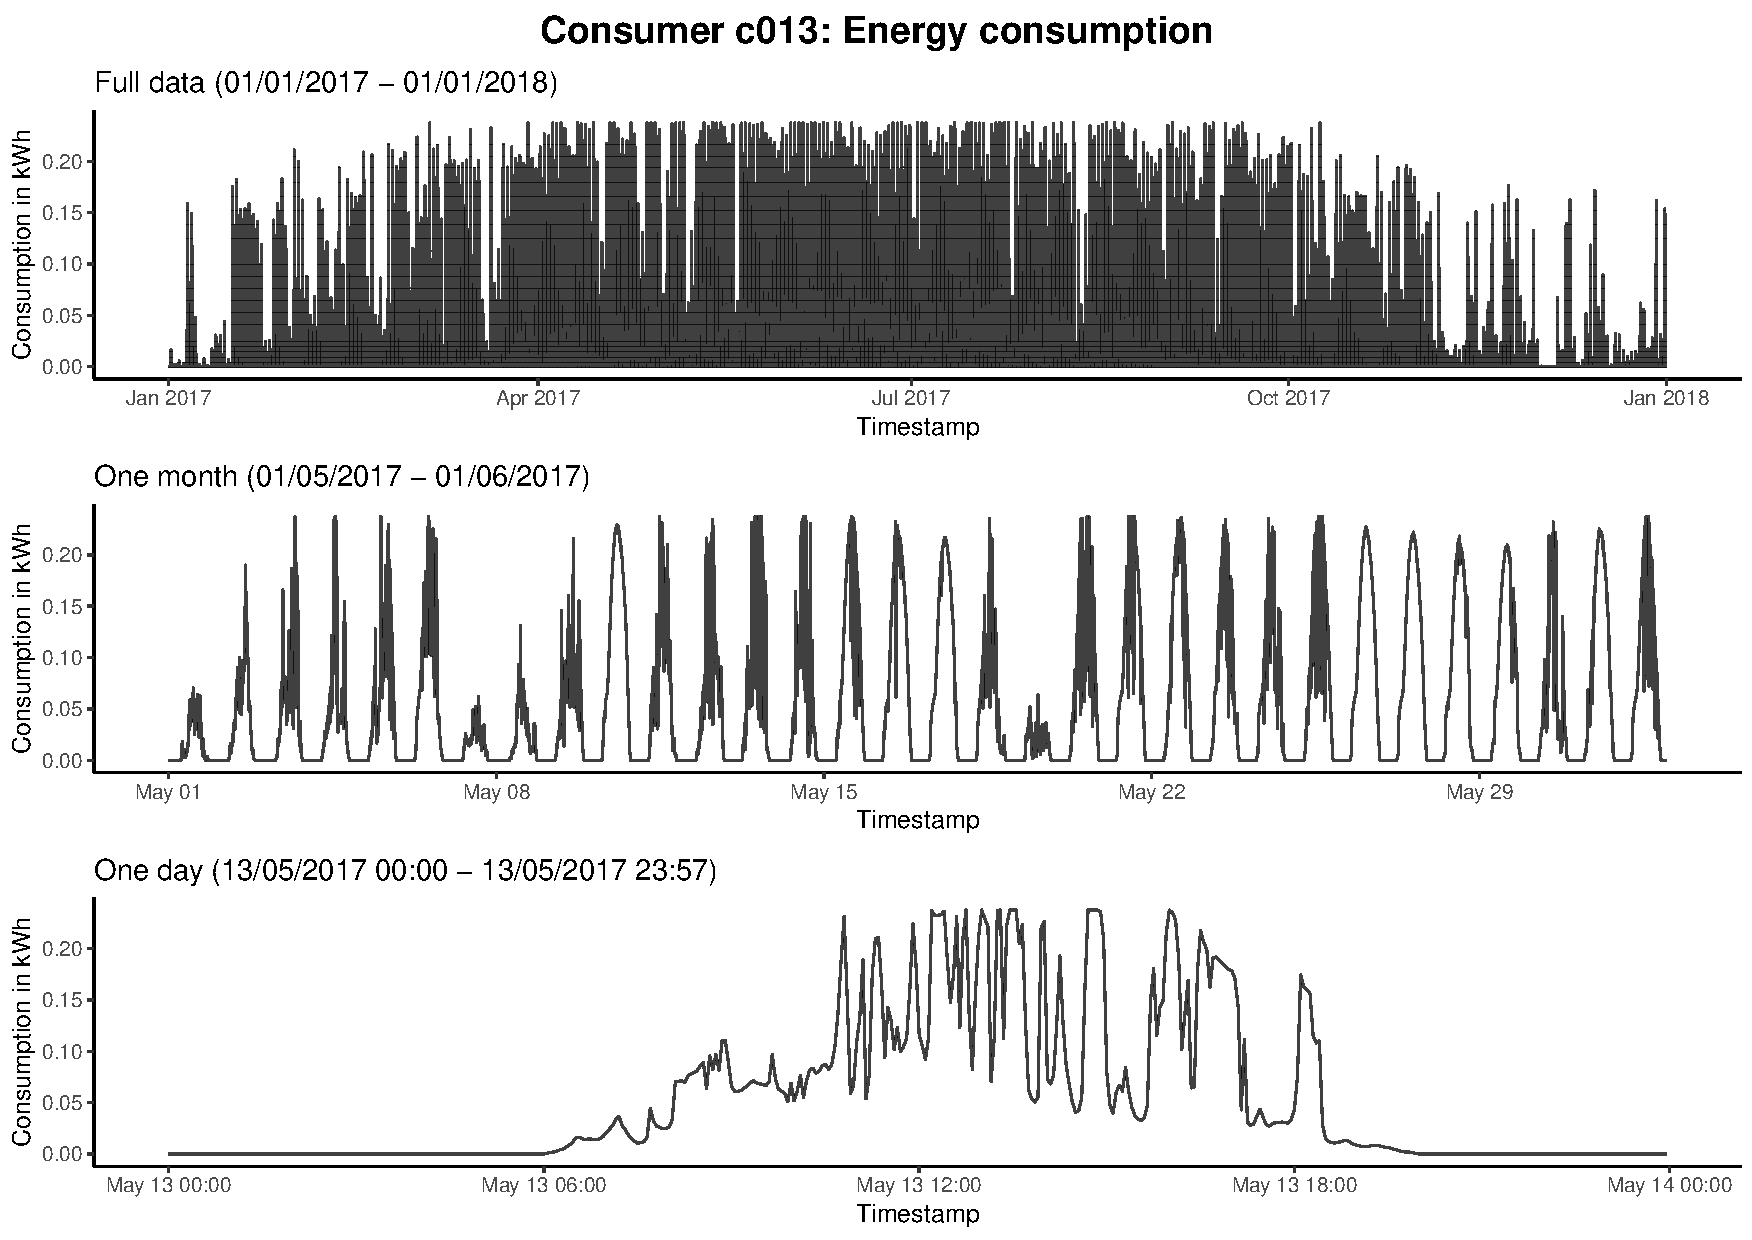
\includegraphics[width=\textwidth]{thesis/graphs/timeseries/c013_cons.pdf}
    \end{minipage}
    \begin{minipage}[ht]{\dimexpr.5\textheight-0.15em}
    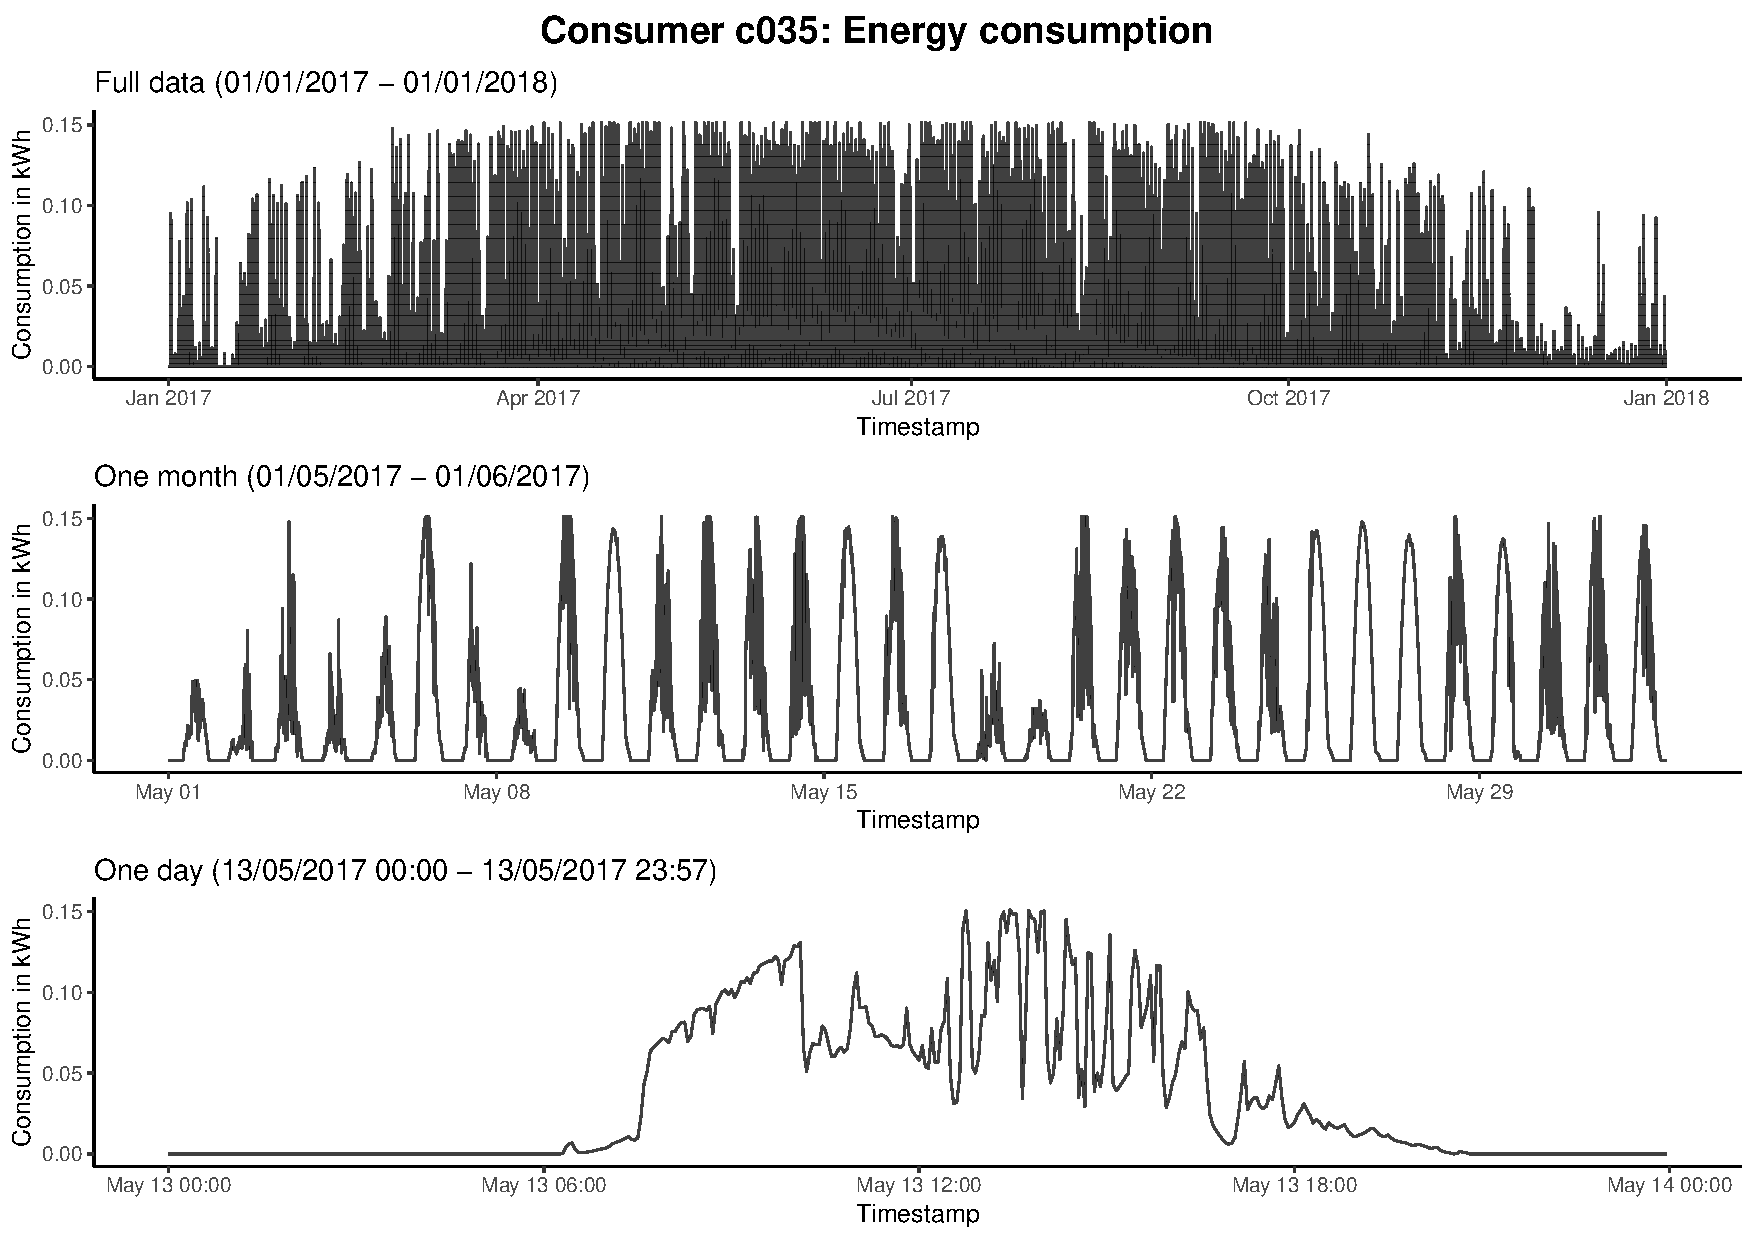
\includegraphics[width=\textwidth]{thesis/graphs/timeseries/c035_cons.pdf}
    \end{minipage}\\
    
    \begin{minipage}[ht]{\dimexpr.5\textheight-0.15em}
    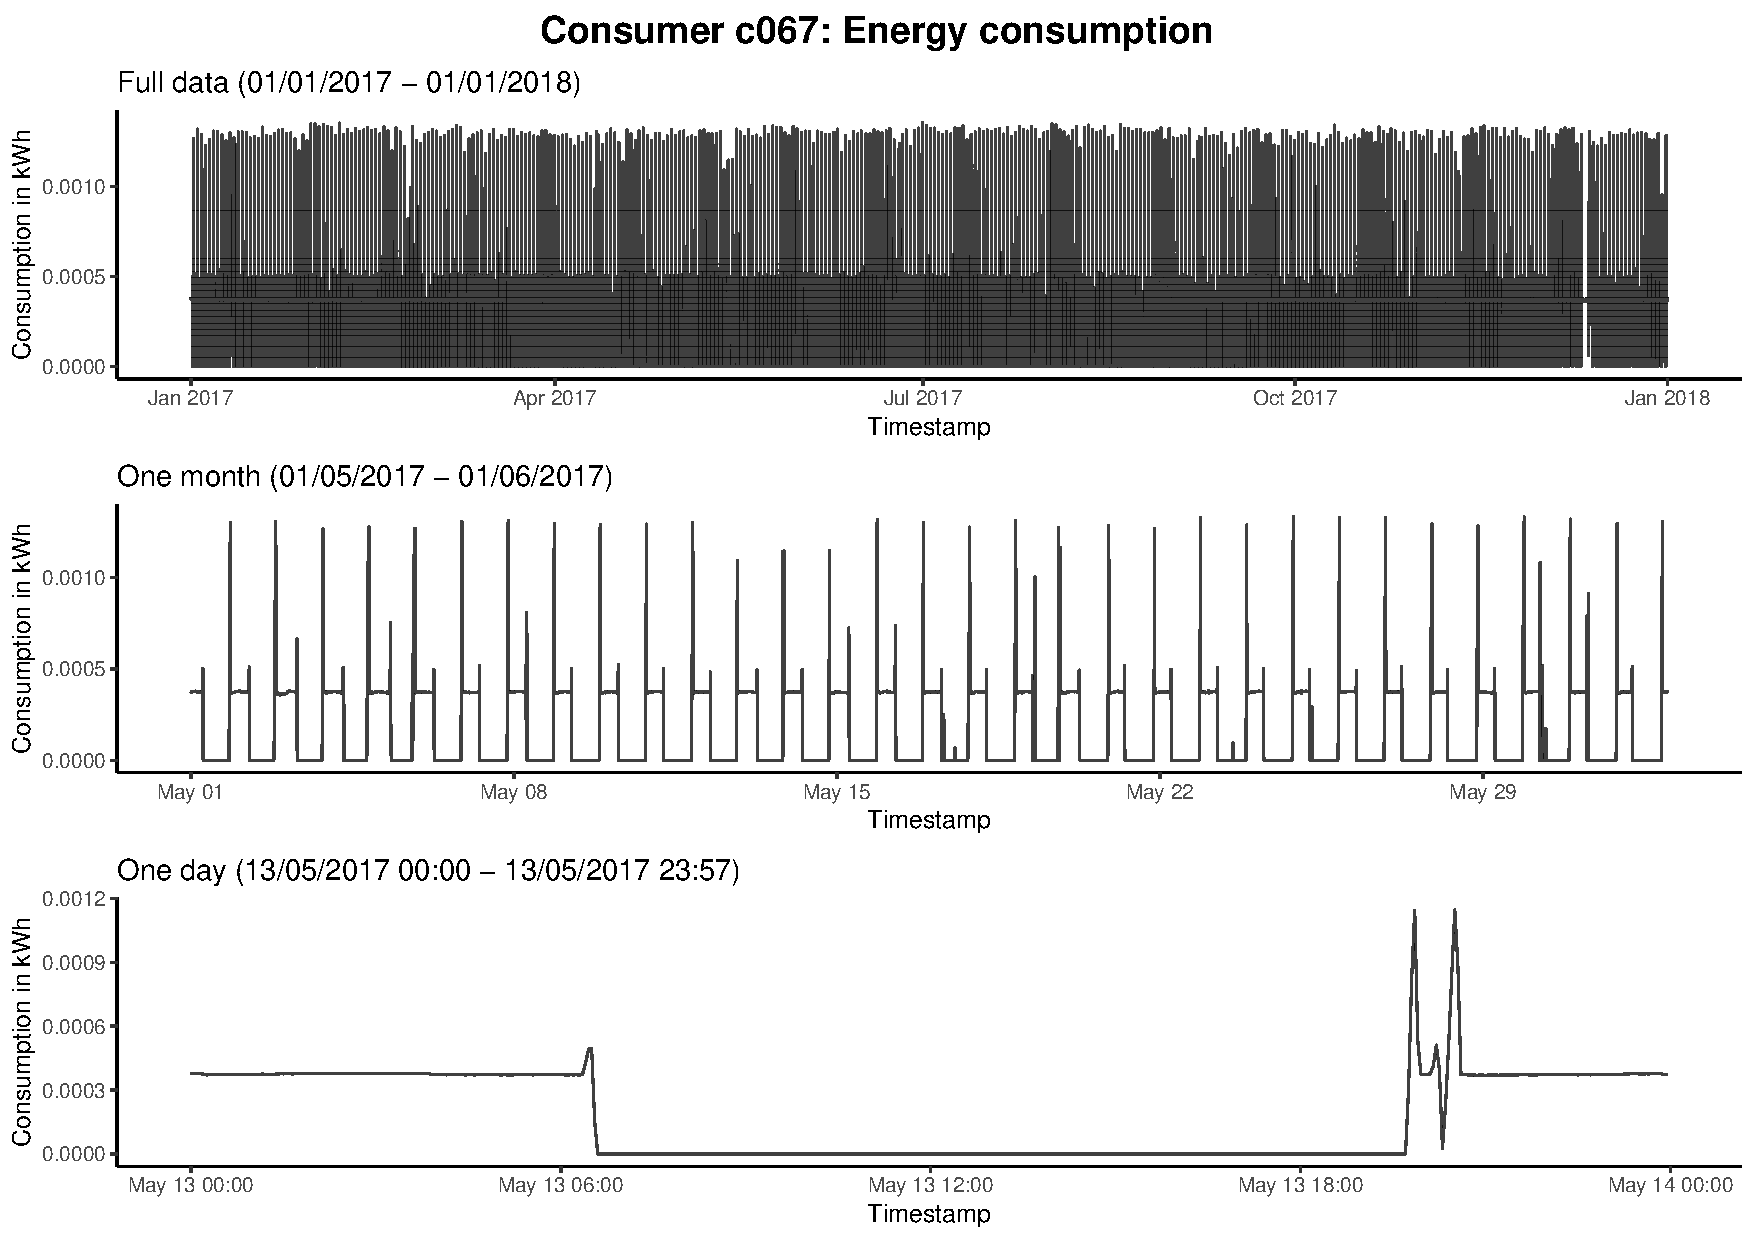
\includegraphics[width=\textwidth]{thesis/graphs/timeseries/c067_cons.pdf}
    \end{minipage}
    \begin{minipage}[ht]{\dimexpr.5\textheight-0.15em}
    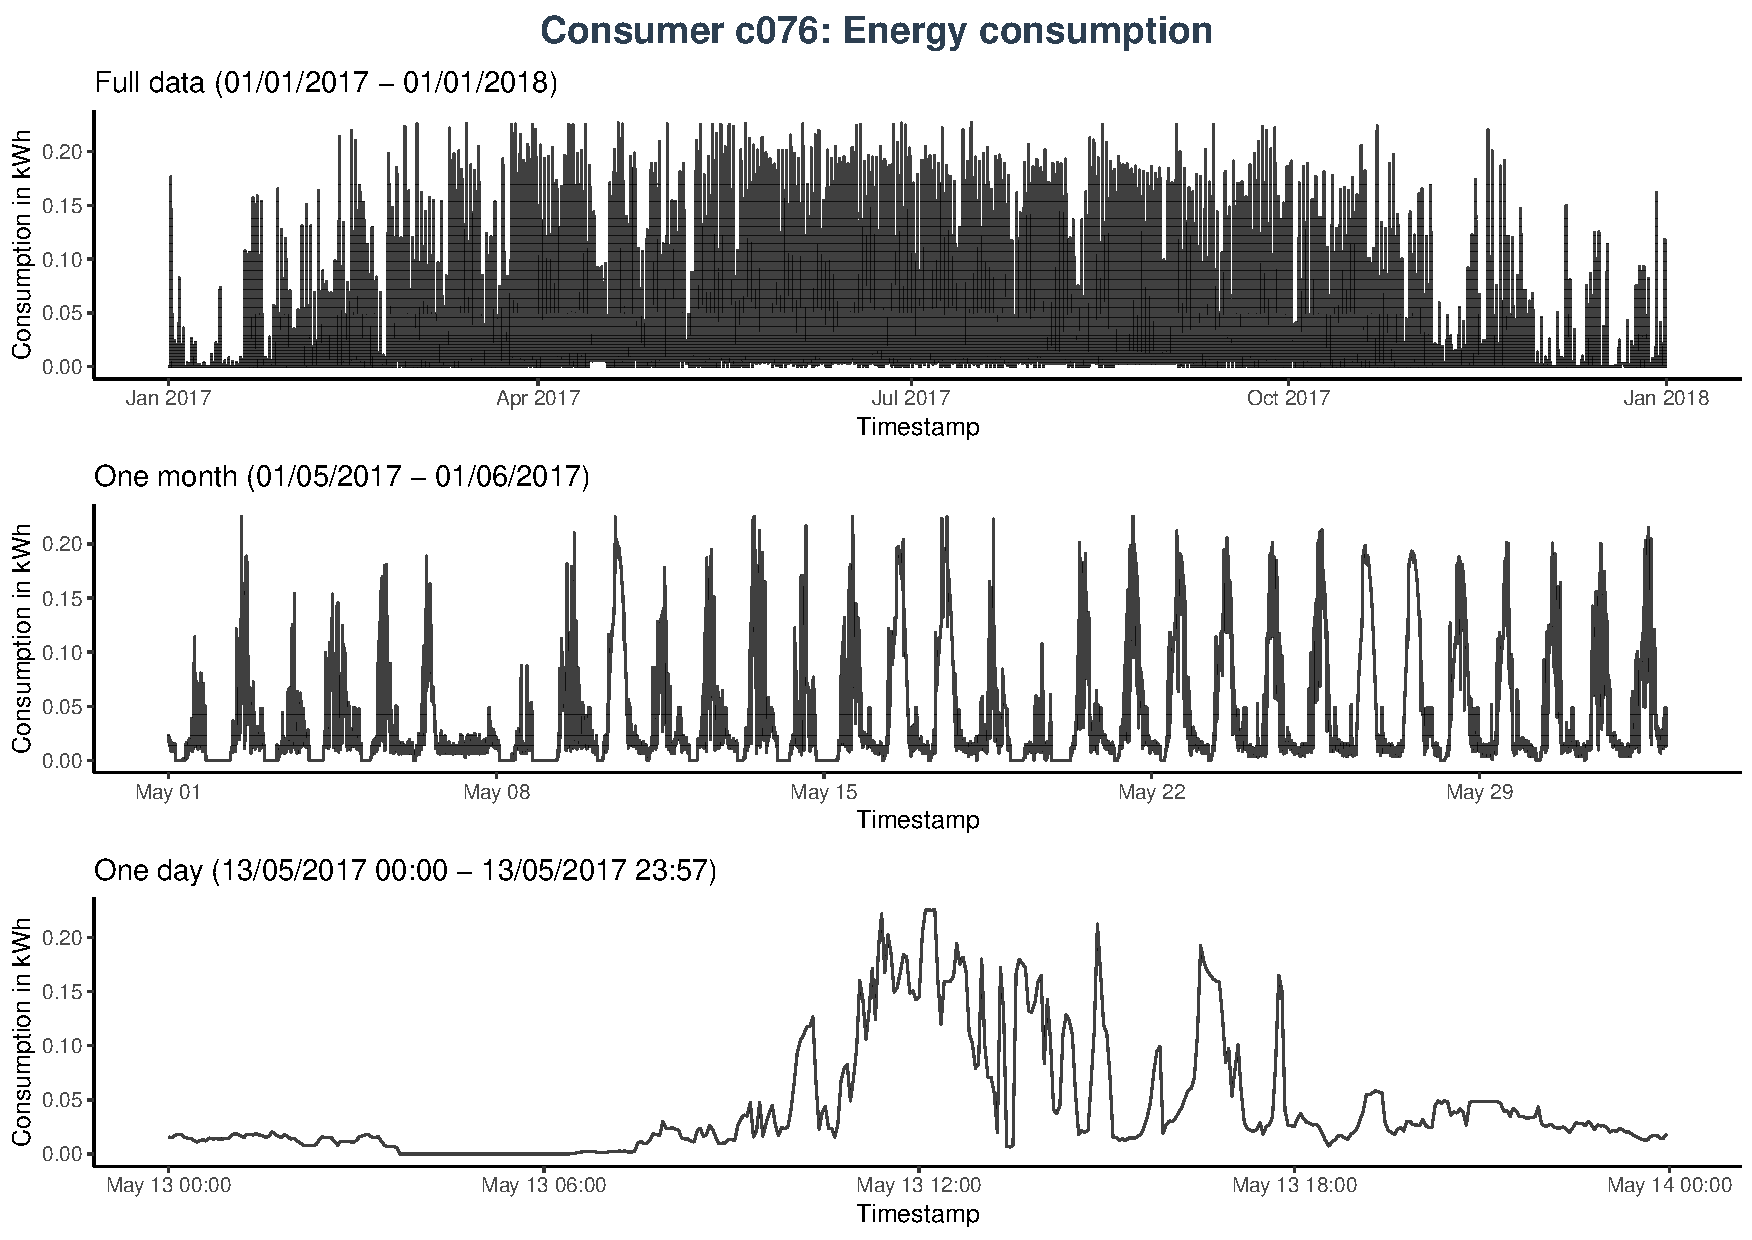
\includegraphics[width=\textwidth]{thesis/graphs/timeseries/c076_cons.pdf}
    \end{minipage}
    
    \caption[Energy consumption recordings of consumers with conspicuous consumption patterns]{Energy consumption recordings of consumers with conspicuous consumption patterns.}
    \label{Fig:consenergycons_peculiar}
\end{sidewaysfigure}

Figure \ref{Fig:consenergycons_peculiar} shows the time series of the aforementioned four consumers with a high share of zero measurements. Consumer 013 and 035 both show a very similar pattern of daily energy consumption. Looking at the middle panel of the two upper graphs in Figure \ref{Fig:consenergycons_peculiar}, the regularity of the consumption increases and decreases for each day is striking. The lower panel shows again, exemplary, May 13. Energy consumption starts to (almost linearly) increase at about 6 a.m. and decreases to 0 kWh at about 6 p.m. This also explains the 52.77 and 54.02 \% of zero values in those to data sets: almost exactly 12 hours per day (from midnight to 6 a.m. and from 6 p.m. to midnight) the consumption is zero, while the energy consumption fluctuates in the meantime with a relatively high "base" consumption. Switching back to the middle panel, it is noticeable that there are some days in May with an even smoother energy consumption increase and decrease over the course of the day. As there is no further socio-demographic data available, we can only guess what the reason for such different consumption patterns are. The most likely explanation seems to be, that the consumption time series of consumer 013 and 035 belongs to a small business rather than to a household.

The lower two graphs show the energy consumption time series of consumer 067 and consumer 075. Consumer 067 consumption pattern zoomed in to one month (middle panel) rather looks like an electrocardiogram than what one would expect from a household energy consumption time series. The regularity of amplitude and frequency is obvious but not easily explained. Consumers 076 consumption pattern looks less suspicious at first sight. However, closer inspection reveals the same daily pattern of increasing consumption throughout the day and very low to zero energy consumption at night. This again rather resembles the energy consumption pattern of a business building or office rooms.



%%%%%%%%%%%
\subsubsection{Prosumer data sets}

For prosumers, peculiarities in the time series pattern can be found either in the net energy consumption or net energy production or in combination. As net energy consumption is much more heterogeneous in the prosumer data sets than in the consumer data sets, it is less obvious what patterns fall outside the norm. However, some prosumer still exhibit obvious anomalies in their consumption patterns. Prosumer 046, 061, and 079 stand out as their consumption is zero for the largest part of the year. This would be an expected pattern if they were net energy producers during this time period. However, as they do not feed in any produced energy at all in 2017, this consumption pattern indicates a data problem. 
Prosumer 038 attracts attention by having a very low total net energy consumption of just 18.168 kWh in 2017 and zero net production. Moreover, this energy is consumed at an extremely low level of around 0.0001 kWh with a standard deviation of $\sigma=2\times10^{-6}$ and just one single drop from this level to zero in the whole year (see Figure \ref{Fig:energycons_p038}). Six more prosumers exhibit a similar pattern of stable level of net energy consumption with occasional drops to zero but no spikes above this stable level. None of them is a net energy producer at any time.

\begin{figure}[htbp]
 \centering
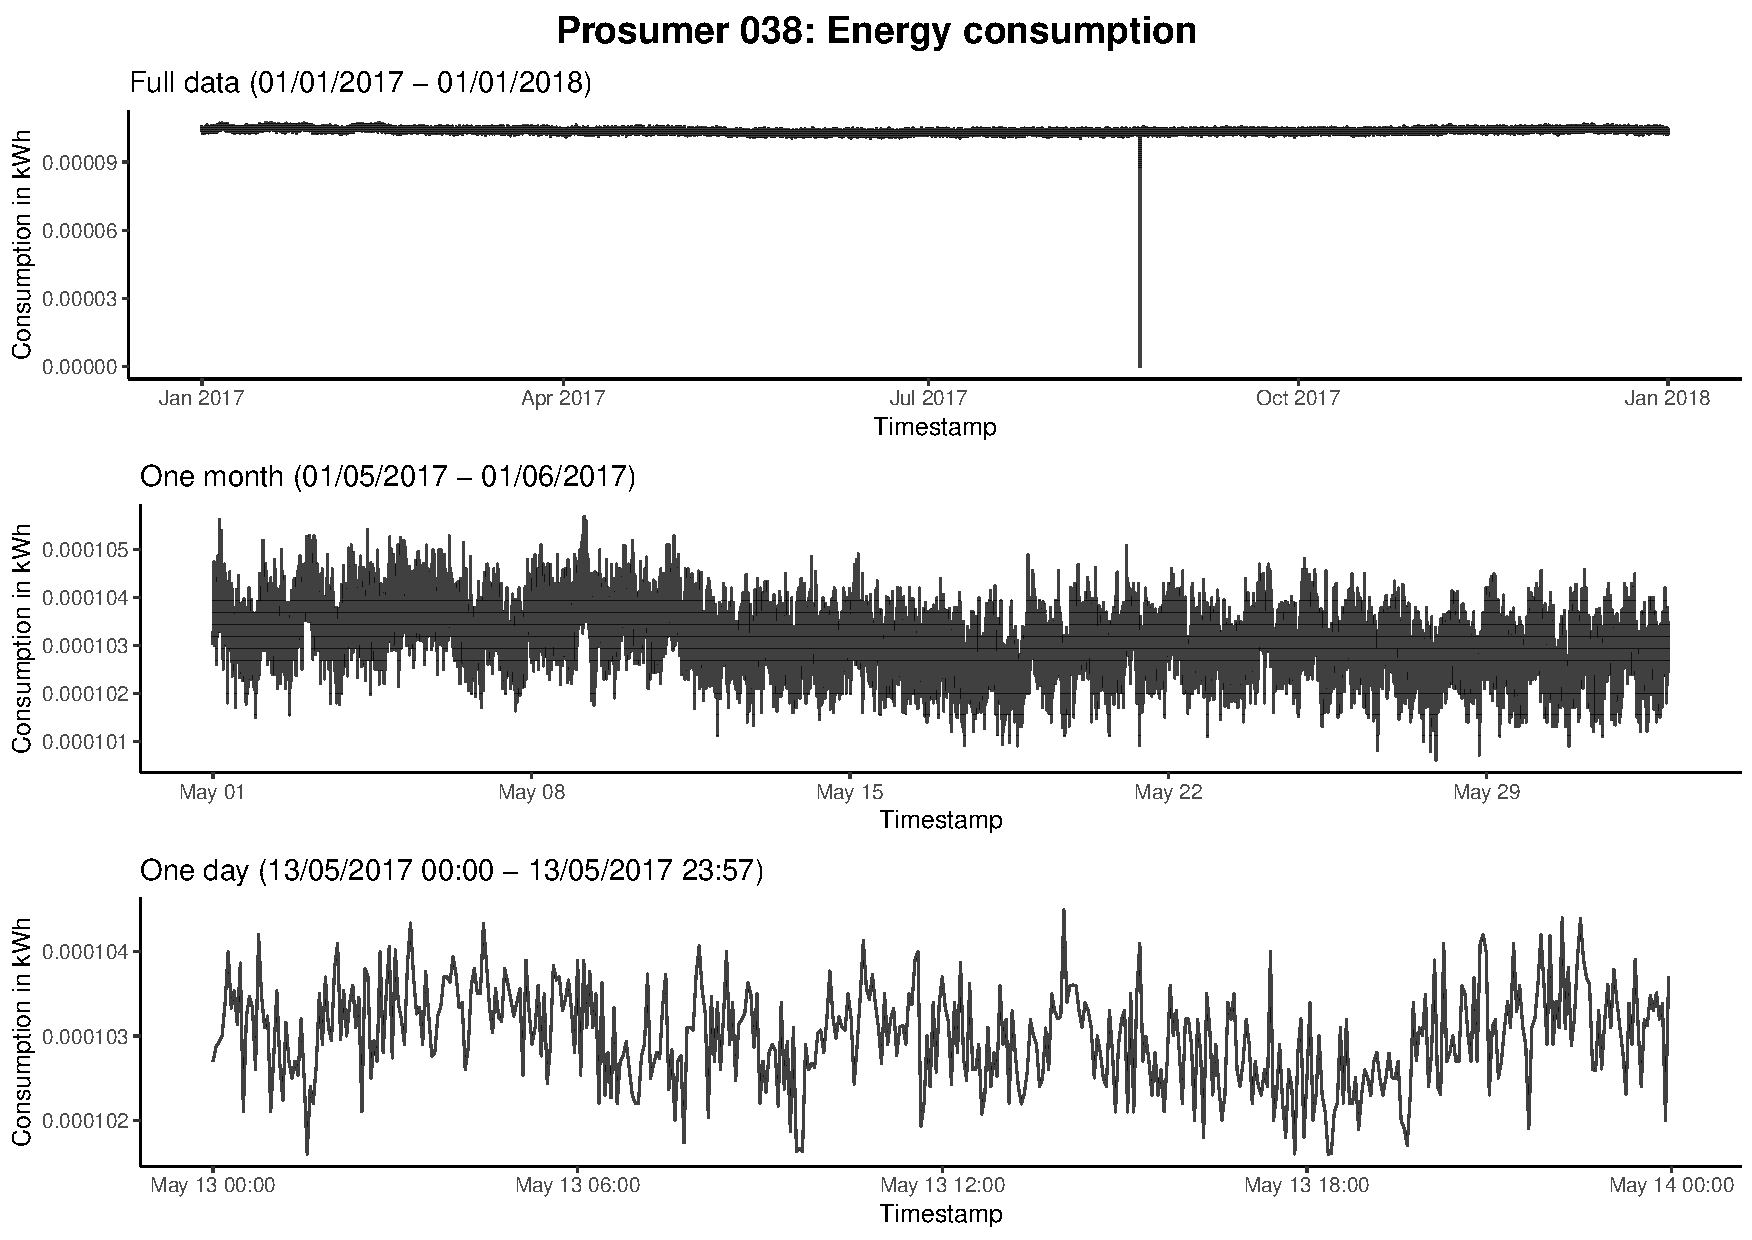
\includegraphics[width=\textwidth]{thesis/graphs/timeseries/p038_cons.pdf}
\caption[Energy consumption recordings of prosumer 038]{Energy consumption recordings of prosumer 038. The first panel shows the full year 2017, the second panel zooms in to one month (May), and the third panel zooms in to one day (May, 13). \quantnet}
\label{Fig:energycons_p038}
\end{figure}

Lastly, prosumer 019 is worth mentioning as it is the only prosumer data set that records a total net energy consumption of 0 kWh for 2017. As the net energy production, however, contains a substantial amount of zero values as well, it seems implausible that prosumer 019 is a regular household. For a household, it appears unlikely that the energy consumption is always zero when the energy production is zero as well.

Regarding the prosumer time series, most of the data sets are peculiar in so far as they have only zero net production values. It seems somewhat unlikely that any household equipped with energy production capacities consumes more than it produces over the whole course of the year at any point in time. However, it is unfortunately not possible to get feedback from Discovergy due to privacy and internal policy reasons on why 84 out of 100 prosumer data sets do not record any energy fed into the grid at all.

Of the remaining 14 data sets, prosumer 084 and 085 stand out as their net energy production time series is almost a flat line at 2.5 kWh per 3-minute interval. Their graphs are shown in Figure \ref{Fig:energyconsprod_p084p085}.

\begin{sidewaysfigure}[htbp]
\centering
\begin{minipage}[h]{\dimexpr.5\textwidth-0.15em}
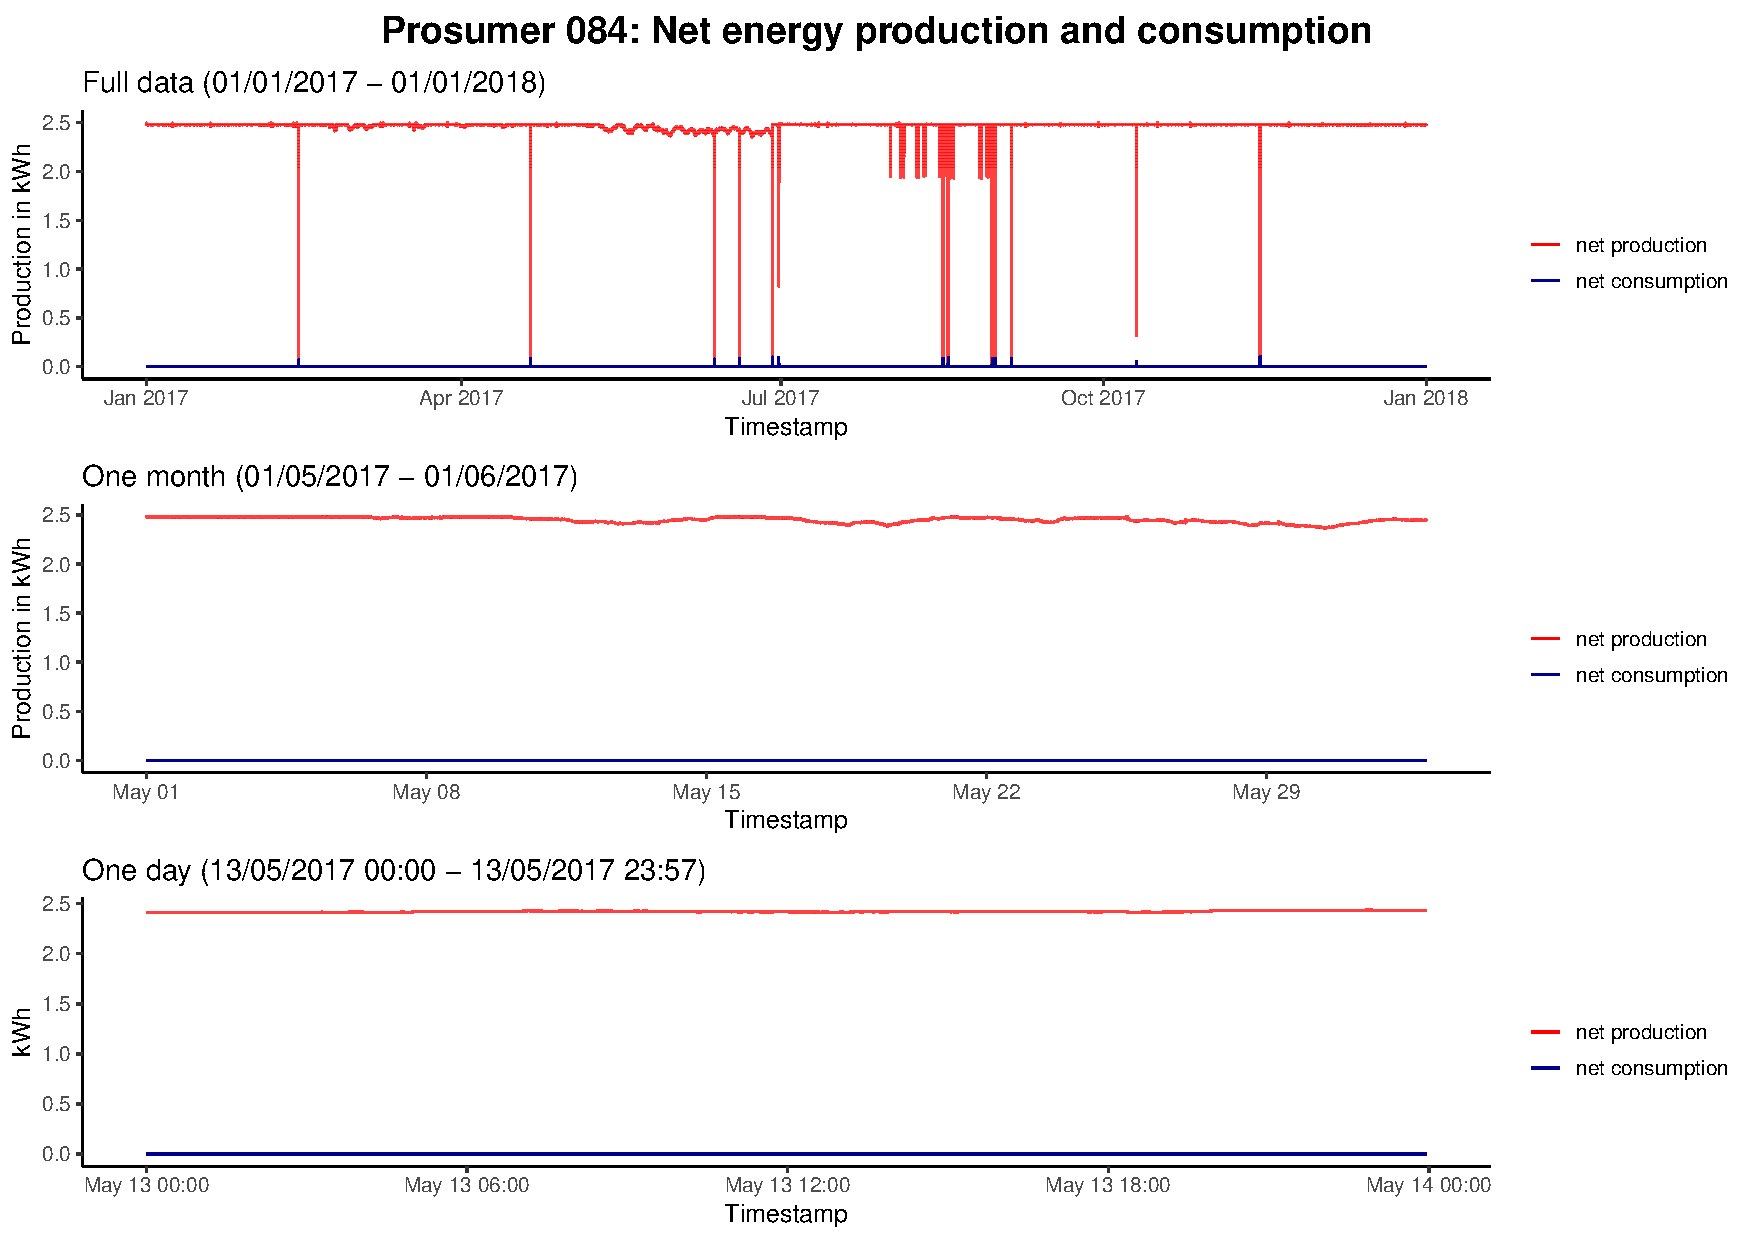
\includegraphics[width=\textwidth]{thesis/graphs/timeseries/p084_prod&cons.pdf}
\end{minipage}
\begin{minipage}[h]{\dimexpr.5\textheight-0.15em}
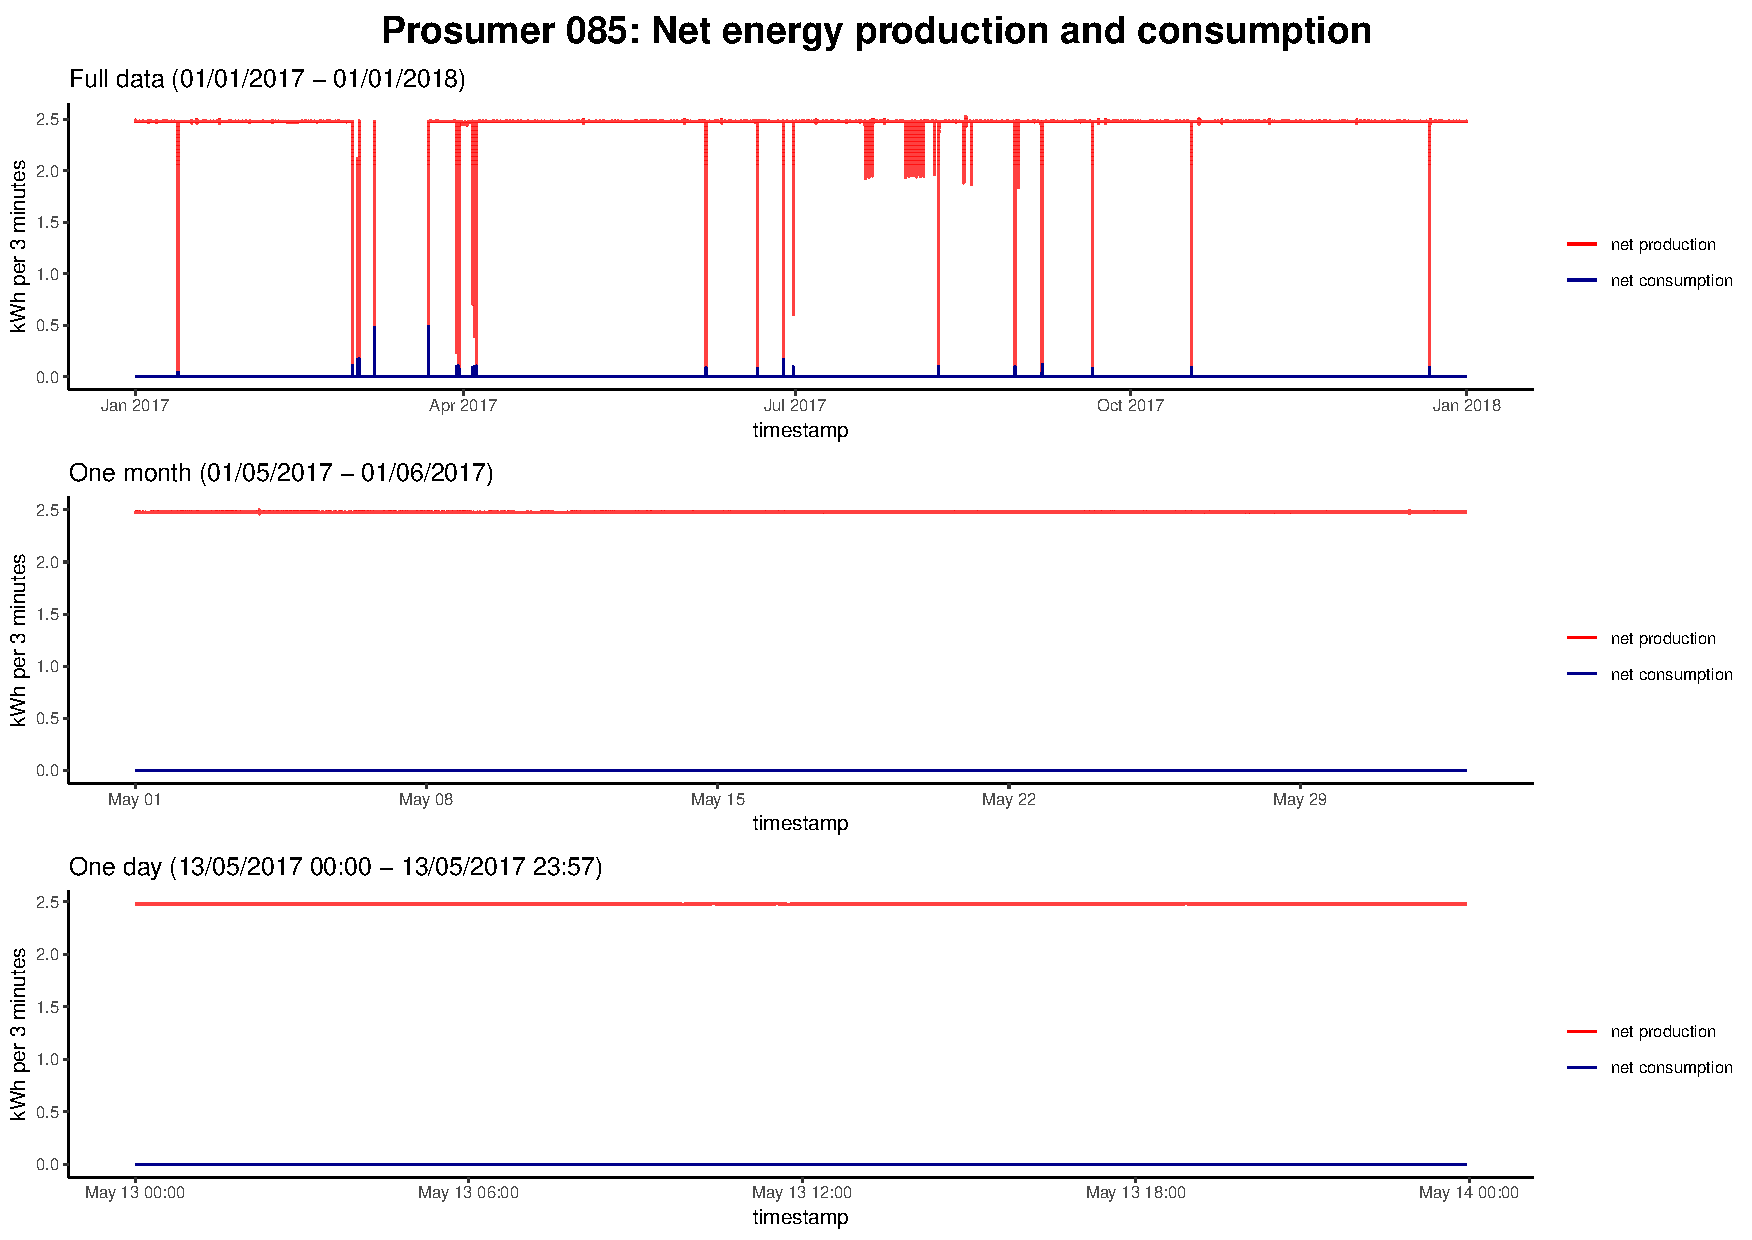
\includegraphics[width=\textwidth]{thesis/graphs/timeseries/p085_prod&cons.pdf}
\end{minipage}

\caption[Energy consumption and production recordings of prosumers 084 and 085]{Energy consumption and production recordings of prosumers 024 and 085. The first panel in the respective graph shows the full year 2017, the second panel zooms in to one month (May), and the third panel zooms in to one day (May, 13). \quantnet}
\label{Fig:energyconsprod_p084p085}
\end{sidewaysfigure}

In conclusion, it seems like the majority of prosumer data sets with non-zero net production values were recorded by smart meters that just record the energy production of a certain installation and not of a household with production capacity. This is not per se a problem, as these installations can act as a individual agent on a local energy market. Even though, they might belong to a household with a separate smart meter, they can sell energy through their own smart meter while the related household's smart meter buys energy. If both smart meters are connected to the same Blockchain wallet, this automatically solves the challenge of pricing the energy relative to the own consumption.

%%%%%%%%%%%%%%%%%%%%%%%%%%%%%%
%%%   Data sets excluded   %%%
%%%%%%%%%%%%%%%%%%%%%%%%%%%%%%

\subsection{Data sets excluded}\label{Sec:Data;Subsec:Exclusion}
The data sets of consumer 013, 035, 067 and 075 shown in Figure \ref{Fig:consenergycons_peculiar} where excluded from the prediction task for the reasons discussed in Section \ref{Sec:Data;Subsec:Peculiarities}. These four consumers plus one additional (consumer 082) exhibited large shares of zero consumption values. Further, consumer 046 was excluded as the consumption time series was flat for the most part of 2017. After some initial fluctuations in the first quarter, all fluctuations stopped entirely. Four more consumers were excluded due to conspicuous regularity in daily or weekly consumption patterns. Lastly, consumer 080 was excluded due to very low and stable consumption values with very rare, extreme spikes. The time series graphs of all additionally to the ones shown in Figure \ref{Fig:consenergycons_peculiar} excluded consumer data sets are shown in Appendix \ref{App:Figures:Excludedc}. Consumer 026 was excluded not due to peculiarities in the consumption patterns but due to missing data. For some unknown reason, the last recorded measurement for consumer 026 is 2017-12-29 07:03:00. As the inclusion of this shorter time series would lead to difficulties in the forecasting algorithms, this data set was excluded as well.

Out of the 100 prosumer data sets, 86 were excluded from the prediction task due to zero total net energy production in 2017. These "prosumers" would not act as prosumers in a local energy market as they never actually supply a production surplus to the market. Moreover, as their net energy production is always zero, their net energy production shows no variation which is a necessary precondition to train any prediction model.

Of the remaining 14 prosumer data sets, prosumer 012 was excluded as the total net energy it fed into the grid in 2017 was just 22.144 kWh. Even though, the feed in occurred continuously over the whole year, it was never exceeded 0.0013 kWh per 3-minute interval with a mean of 0.0001 kWh, which is too small to be of interest. Prosumer 015 was excluded as it only fed energy into the grid in the period from 06.01.2017 to 19.01.2017. For all other measurement points the net energy production was zero. The time series graph of the two excluded prosumer data sets with production data are shown in Appendix \ref{App:Figures:Excludedp}

Hence, 88 consumer and 12 prosumer data sets remained for the following prediction tasks. All data sets included a time stamp and the consumption time series for consumers respectively the production time series for prosumers with a total of 175,200 data points each.


%%%%%%%%%%%%%%%%%%%%%%%%%%%%%%%%%%%%%%%%%%%%%%%%%%%%%%%%%%%%%%%%%


\newpage

\section{Results}\label{Sec:Results}

The results will be presented in two parts: First, the forecasting accuracy of the prediction models is evaluated and presented. Second, the results of the market simulation -- which is run once with the true consumption and production values and once with the predicted values -- are reported.


%%%%%%%%%%%%%%%%%%%%%%%%%%%%
%%%   Benchmark models   %%%
%%%%%%%%%%%%%%%%%%%%%%%%%%%%

\subsection{Evaluation of the prediction models}\label{Sec:Results;Subsec:Forecast}

Three prediction methods where used to forecast the energy consumption of 88 consumer data sets and to forecast the energy production of 12 prosumer data sets: a benchmark model (see Section~\ref{Sec:Method;Subsec:Benchmark}), a LSTM RNN model (see Section~\ref{Sec:Method;Subsec:LSTM}), and a LASSO model (see Section~\ref{Sec:Method;Subsec:LASSO}). All three prediction models were compared and evaluated using the error measures presented in Section~\ref{Sec:Method;Subsec:Error}.


%%%%%%%%%%%
\subsubsection{Consumption data}

The performance of the prediction models was tested on a quarter of the available data. That is, the prediction models were fitted on the consumption values from 01.01.2017~00:00 to 30.09.2017~00:00 which is equivalent to 131,040 data points per data set. For all 88 consumer data sets, the models were fitted separately resulting in as many distinct LASSO and LSTM prediction models. The fitted models were then used to make energy consumption predictions in 15-minute intervals for each household individually on the data from 01.10.2017~00:00 to 01.01.2018~00:00. This equates to 8,836 predicted values per data set per prediction method.

Figure~\ref{Fig:glimpse_predcons} exemplary shows the true and predicted consumption values of consumer 011 on October 27, 2017. The naive benchmark model just follows the true consumption shifted by one time step (i.e. 15 minutes). This fits the true values generally good, as long as there are no sudden jumps in the household's energy consumption. Spikes in energy consumption, as in this example one occurred in the 15 minutes before 07:30 and 08.30 respectively, necessarily lead to two periods with high errors of the naive predictor: First, once the jump to a high consumption level occurs and the naive predictor remains at the previous low level, and second, once the consumption suddenly returns to the low ``baseline" consumption level and the naive predictor lags behind at the high level of the previous period. In such situations, the LASSO and LSTM models are more accurate. Even though, they underestimate the jumps in energy consumption, they do not lag behind as much as the naive predictor and, generally, have the ability to anticipate movements. However, the exemplary glimpse onto the predicted consumption values of consumer 011 already reveals that also the sophisticated prediction models lack the ability to accurately predict sudden movements in the energy consumption and tend to overestimate low consumption levels and underestimate spiking energy consumption.
%
\begin{figure}[htbp]
    \centering
    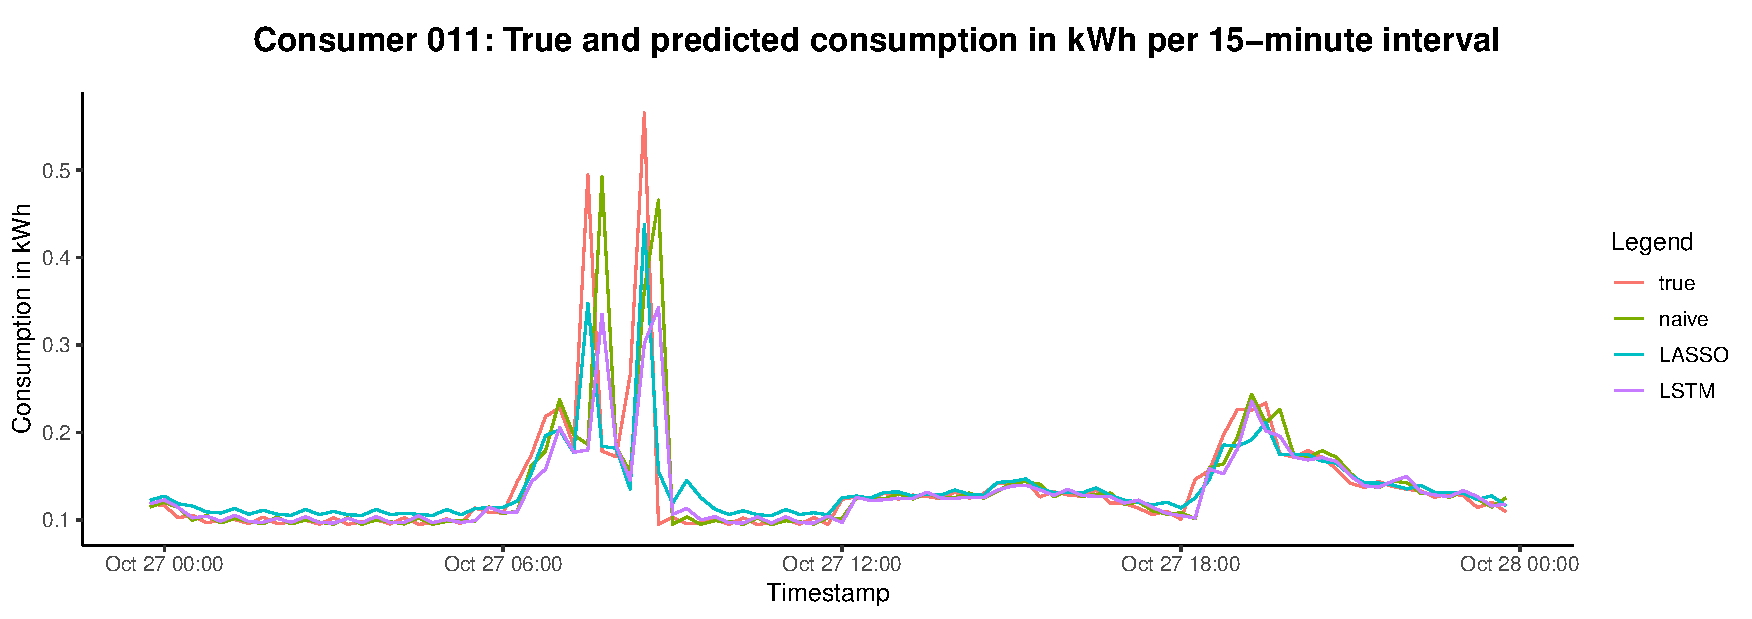
\includegraphics[width=\textwidth]{thesis/graphs/evaluation/c011_pred_cons.pdf}
    \caption[Exemplary 24 hours of true and predicted consumption values]{Exemplary 24 hours of true and predicted consumption values of consumer 011. \quantnet\href{}{}}
    \label{Fig:glimpse_predcons}
\end{figure}
%

Systematically analyzing the total over- and underestimation of the different prediction models on each consumer data set confirms this impression. Figure~\ref{Fig:overunderestimation} displays the total sum of over- and underestimation errors of each prediction method per data set. As one would expect, the naive benchmark model consistently over- and underestimated by the same amount per data set. The reason for that is, that the sum of over- and underestimation errors only depends on the amplitude of the jumps in the case of the naive predictor. Thus, overestimation errors occur in the same frequency and magnitude as underestimation errors. The LASSO model achieved overall lower total sums of errors than the benchmark model. Moreover, the sum of underestimation errors is higher across the data sets than the sum of overestimation errors. This points towards a general tendency of underestimating sudden increases in energy consumption by the LASSO model. The LSTM model on the other hand shows a much higher variability in the sums of over- and underestimation errors. By tendency, the overestimation errors of the LSTM model were smaller than those of the LASSO and benchmark models. Nevertheless, the underestimation is much more pronounced in the case of the LSTM model. Especially, some data sets stand out regarding the high sum of underestimation errors. This points towards a much higher heterogeneity in the suitability of the LSTM model to predict consumption values depending on the energy consumption pattern of the specific data set. The LASSO model on the other hand seems to be more equally well suited for all data sets and their particular consumption patterns.
%
\begin{figure}
    \centering
    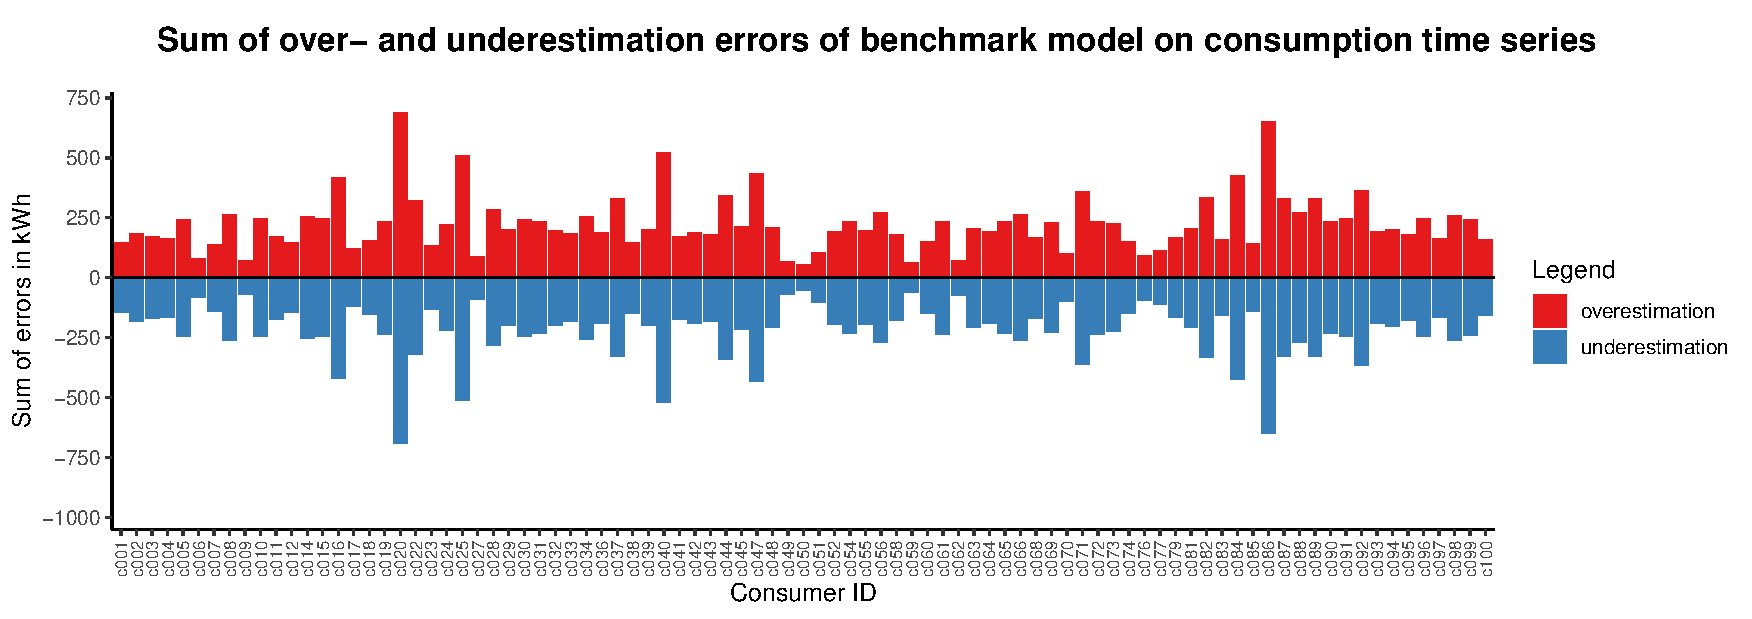
\includegraphics[width=\textwidth]{thesis/graphs/evaluation/c_barplot_naive_overunderestimation.pdf}\\\vspace{.6cm}
    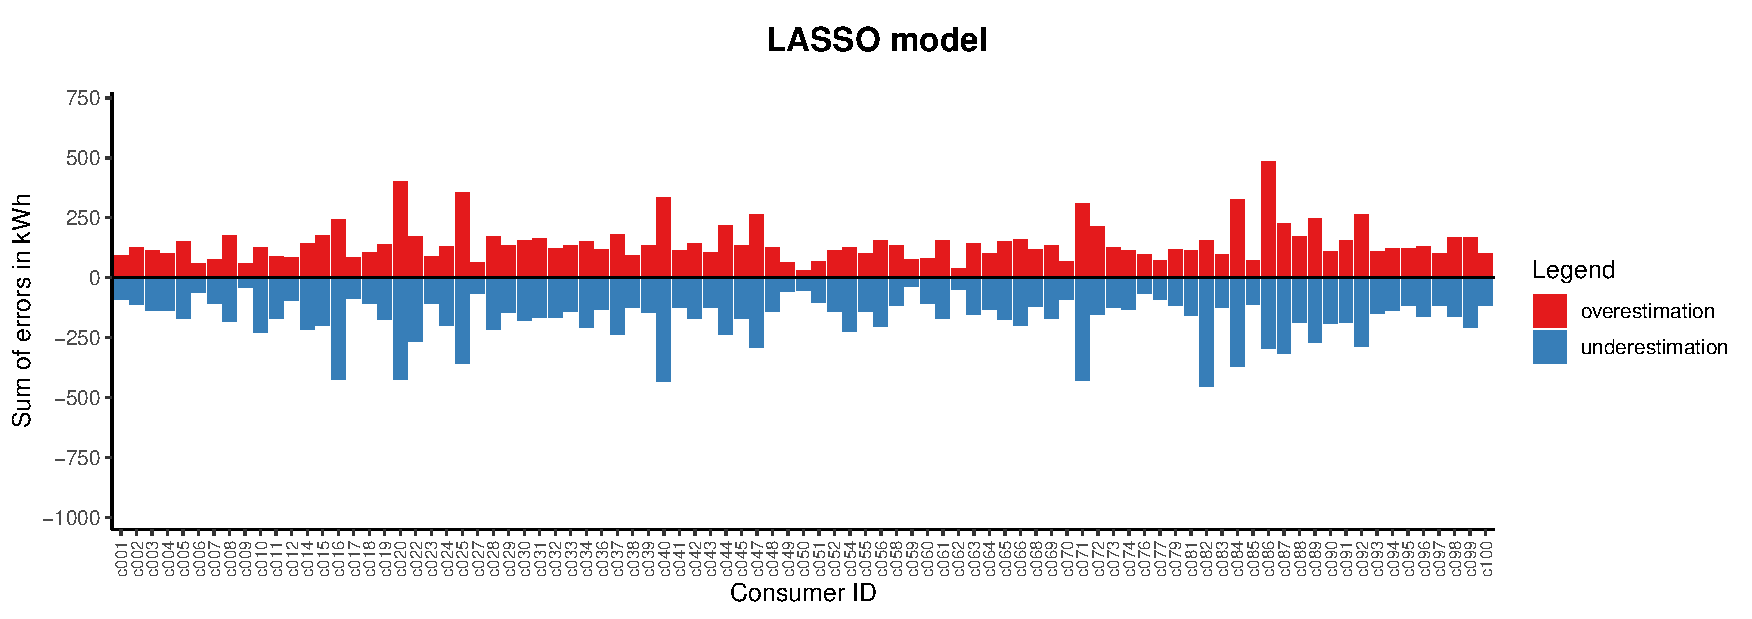
\includegraphics[width=\textwidth]{thesis/graphs/evaluation/c_barplot_LASSO_overunderestimation.pdf}\\\vspace{.6cm}
    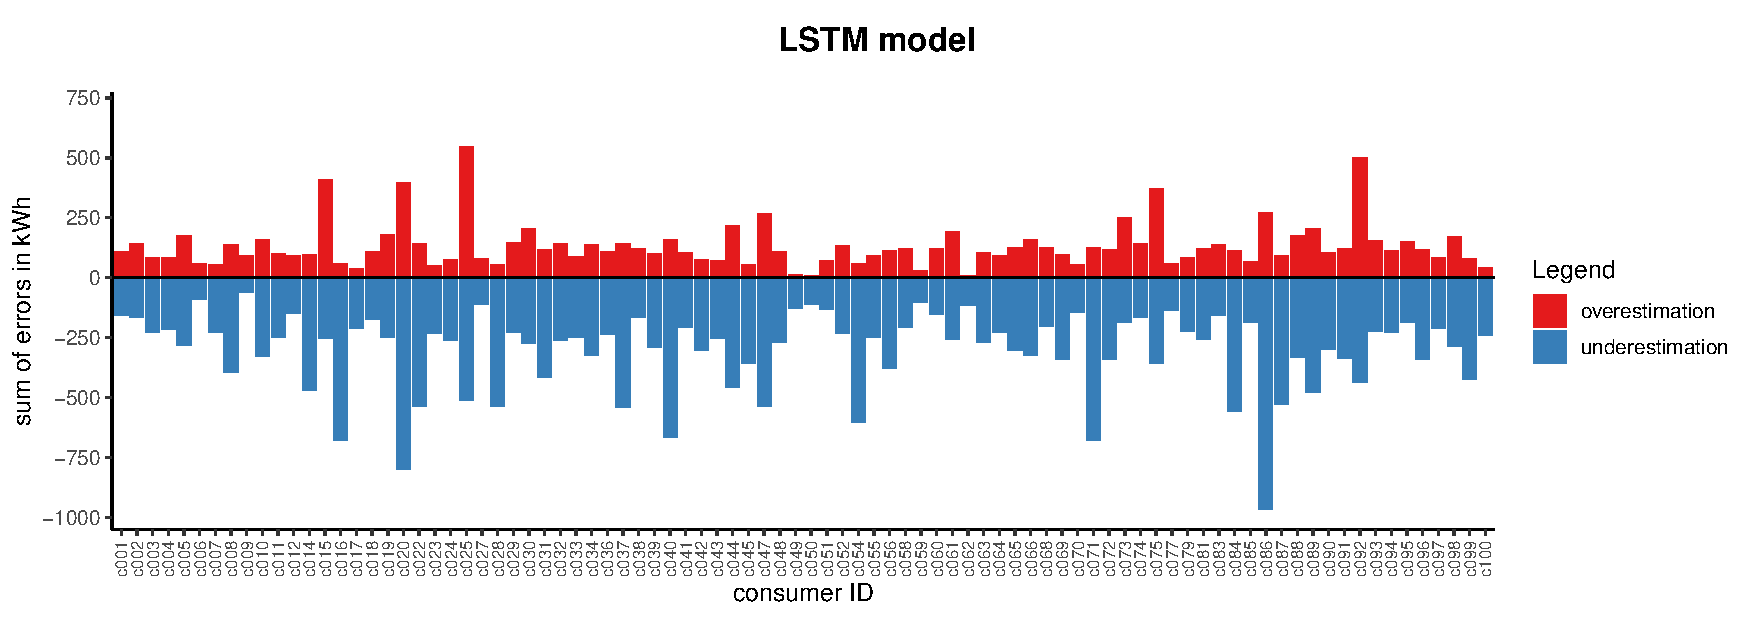
\includegraphics[width=\textwidth]{thesis/graphs/evaluation/c_barplot_LSTM_overunderestimation.pdf}
    \caption[Sum of total over- and underestimation errors per consumer data set]{Sum of total over- and underestimation errors of energy consumption per consumer data set and prediction model. \quantnet\href{}{}}
    \label{Fig:overunderestimation}
\end{figure}
%

The average performance of the three prediction models across all 88 data sets is shown in Table~\ref{Tab:avg_errormeasures}. As can be seen, LASSO and LSTM consistently outperform the benchmark model according to MAE, RMSE, MAPE, and MASE\footnote{Note, that the MASE score of the benchmark model must be exactly one as the MASE is defined as the mean absolute error absolute to the MAE of the naive predictor (see Equation~\ref{Eq:naivepred}).}. Interestingly, due to the heavy penalty NRMSE puts on comparably large prediction errors, both sophisticated prediction methods, however, perform worse according to NRMSE. A detailed analysis of this unexpected result reveals that it is mainly driven by an extremely bad NRMSE score for LSTM and LASSO on merely one out of the 88 data sets. As can be seen in Figure~\ref{Fig:heatmaps}, the predictions on consumer data set 027 have a particularly high NRMSE (and MAPE) compared to all other data sets. However, this pattern is not present in the absolute error measures.
%
\begingroup\catcode`"=9
\begin{table}[ht]
{\footnotesize
    \csvreader[centered tabular=l|SSSSS,
    before reading=\sisetup{round-mode=places,round-precision=2,round-integer-to-decimal},
    filter not strcmp={\thecsvinputline}{1},
    table head=
    \hline\hline
     \multicolumn{1} {l}{\textbf{Model}} & \multicolumn{1} {c}{\textbf{MAE}} & \multicolumn{1} {c}{\textbf{RMSE}} & \multicolumn{1} {c}{\textbf{MAPE}} & \multicolumn{1} {c}{\textbf{NRMSE}} & \multicolumn{1} {c}{\textbf{MASE}}\\
    \hline,
    no head,
    separator=comma,
    respect all,
    late after line=\\,
    table foot=\hline \hline]
    {thesis/tables/avg_errorMeasures_c.csv}{}%
    {\csvcolii & \csvcoliii & \csvcoliv & \csvcolv & \csvcolvi & \csvcolvii}}%
    \caption[Mean of error measures for all 82 consumer data sets]{Mean of error measures for the prediction of energy consumption across all 82 consumer data sets. \quantnet\href{ }{}}
    \label{Tab:avg_errormeasures}
\end{table}
\endgroup
%

%
\begin{figure}[htbp]
 \centering
 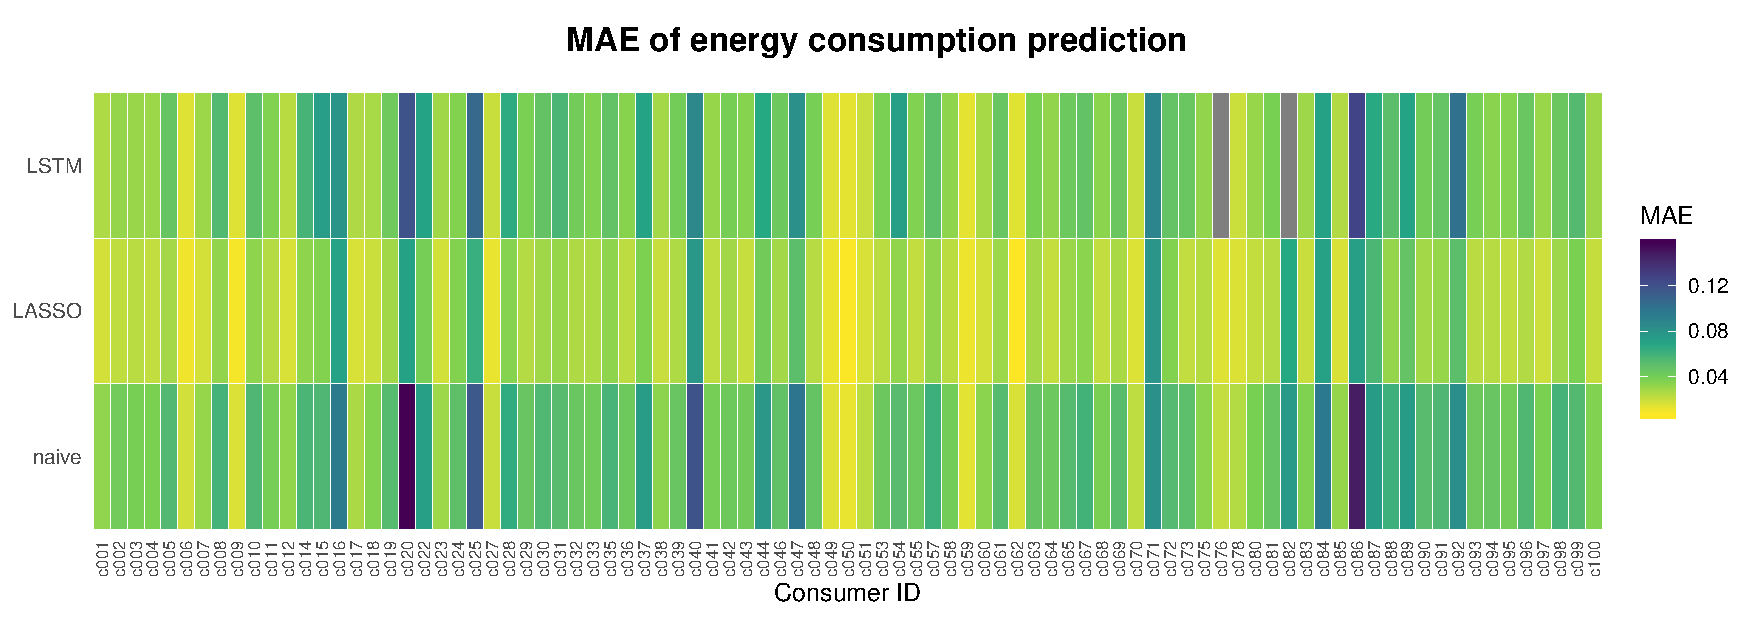
\includegraphics[width=\textwidth]{thesis/graphs/evaluation/c_heatmap_MAE.pdf}
 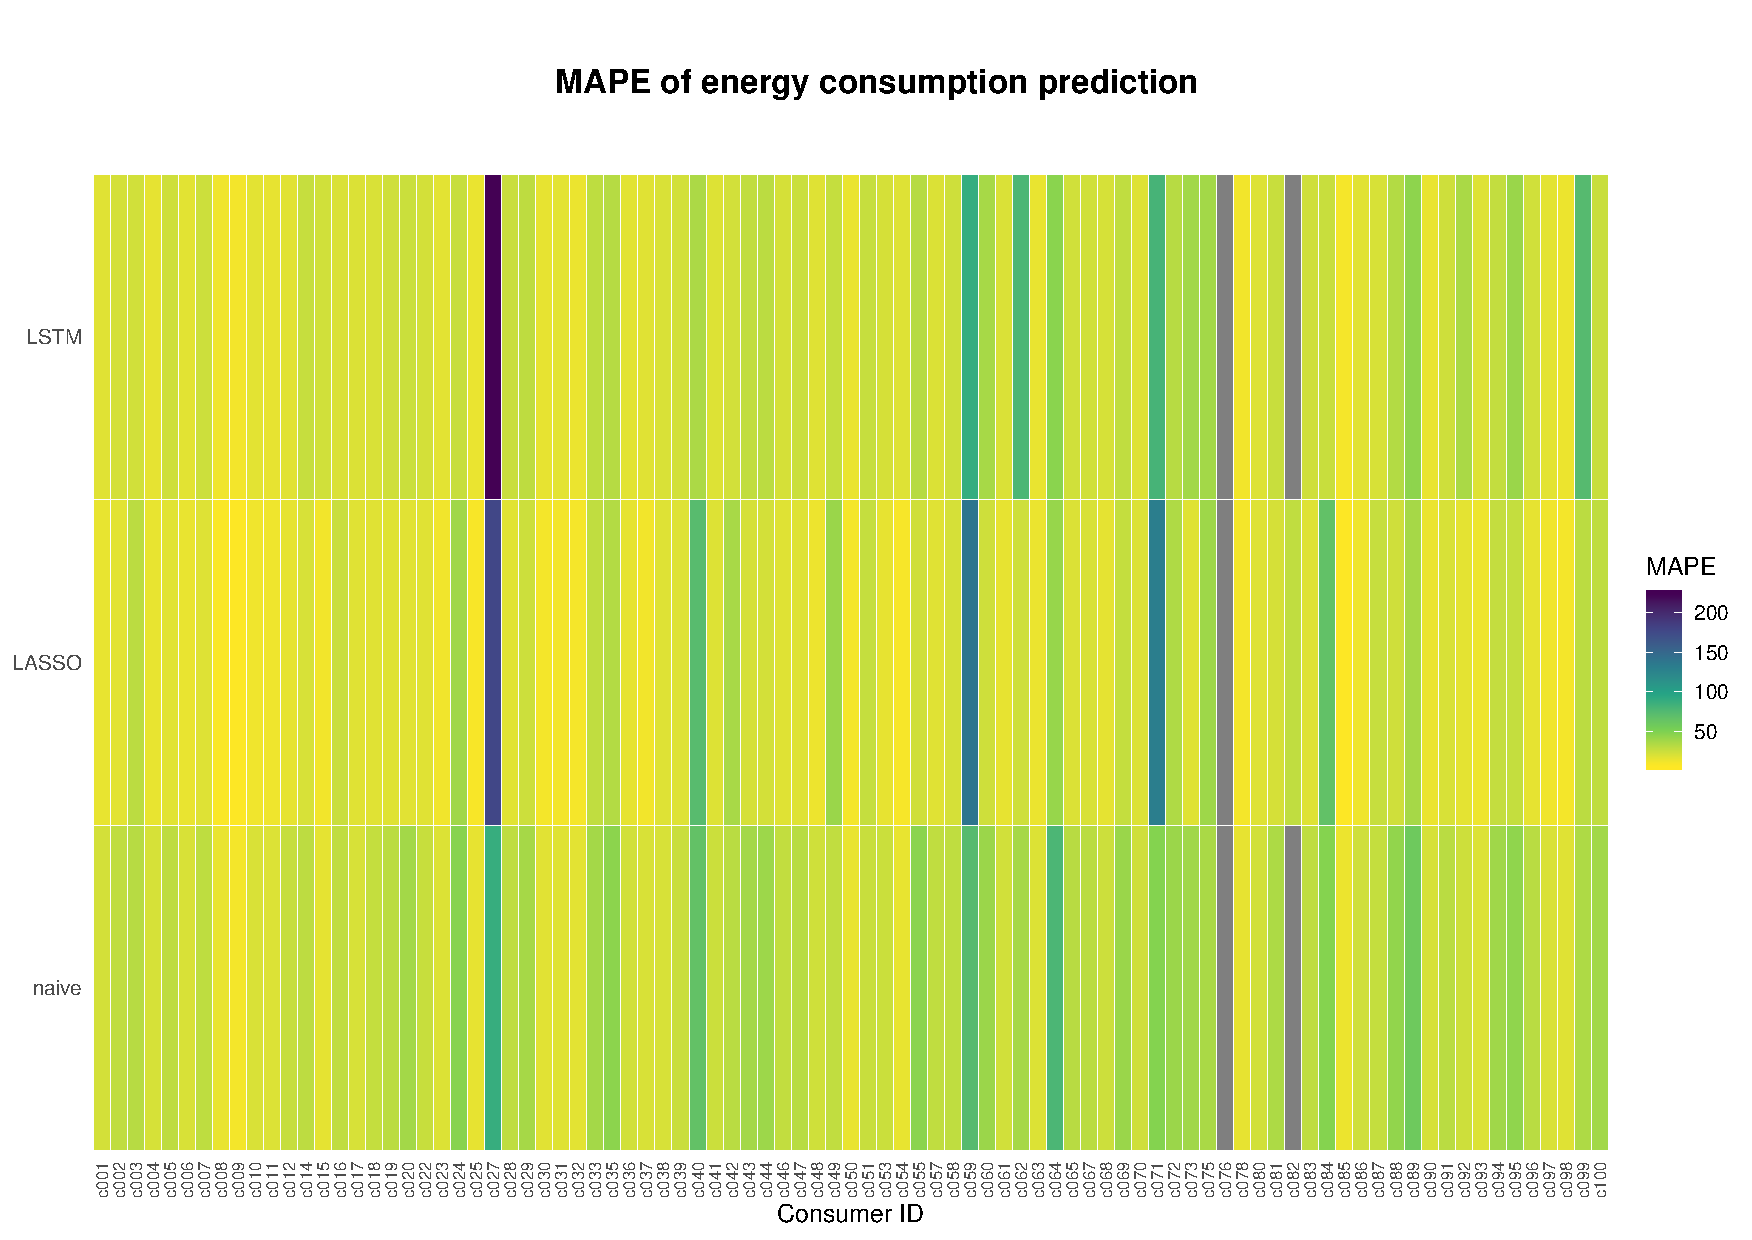
\includegraphics[width=\textwidth]{thesis/graphs/evaluation/c_heatmap_MAPE.pdf}
 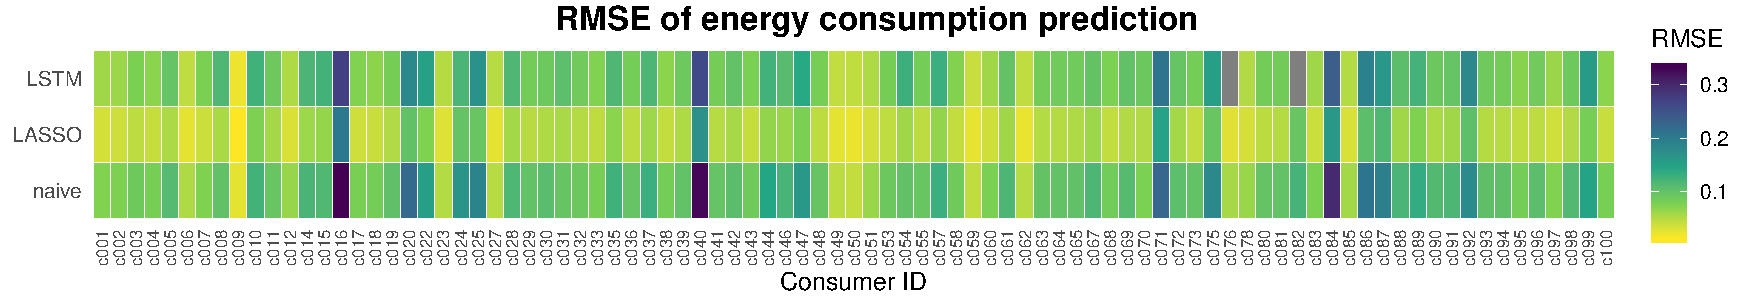
\includegraphics[width=\textwidth]{thesis/graphs/evaluation/c_heatmap_RMSE.pdf}
 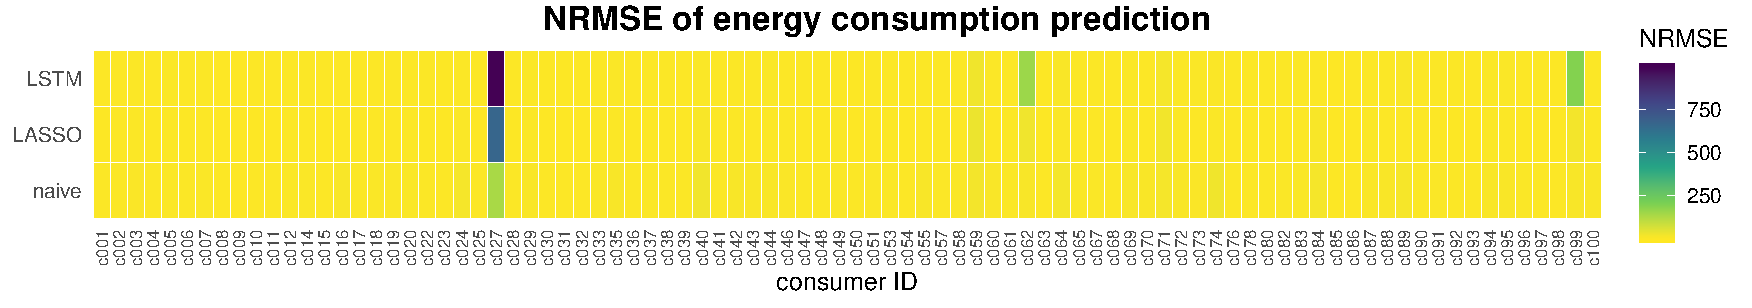
\includegraphics[width=\textwidth]{thesis/graphs/evaluation/c_heatmap_NRMSE.pdf}
 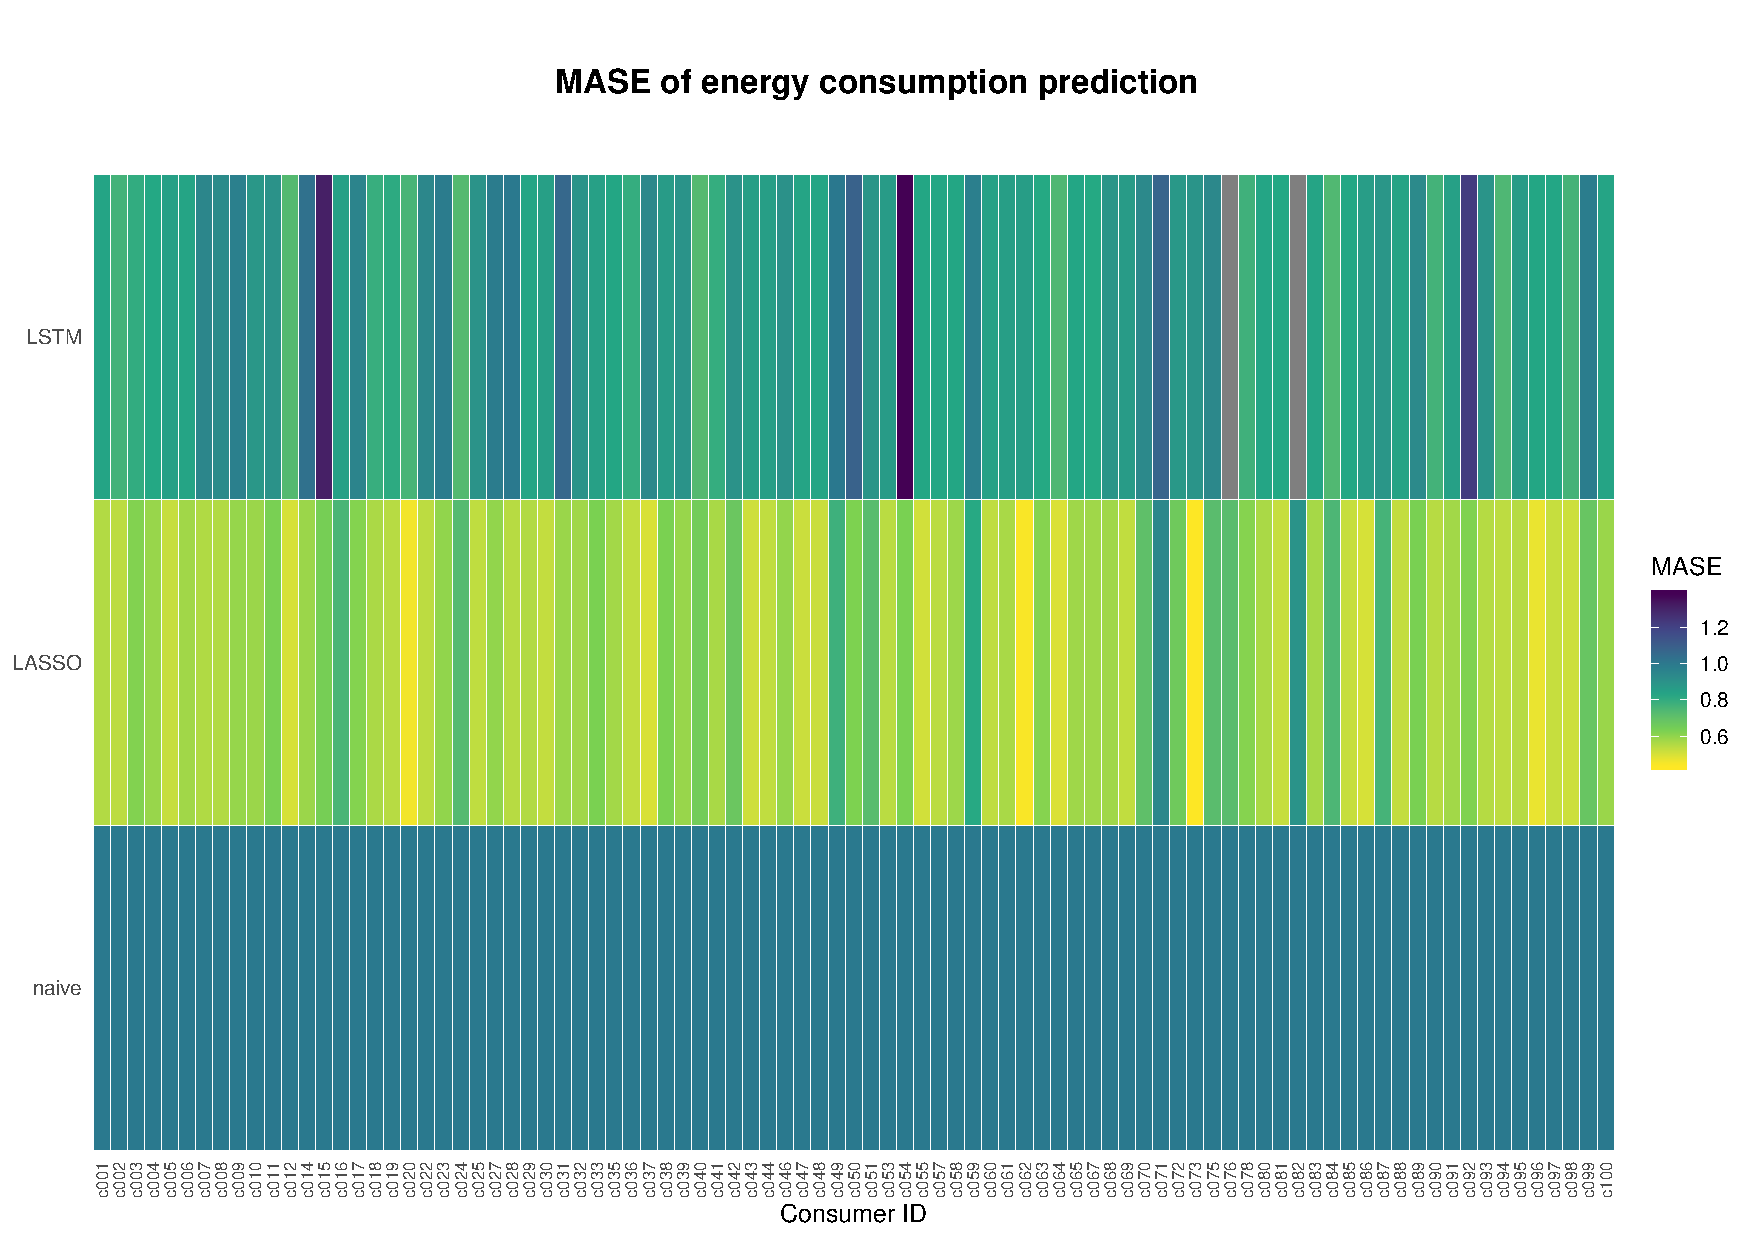
\includegraphics[width=\textwidth]{thesis/graphs/evaluation/c_heatmap_MASE.pdf}
\caption[Heatmaps of all error measures for consumption values]{Heatmap of MAE, MAPE, RMSE, NRMSE, and MASE scores for the prediction of consumption values per consumer data set. \quantnet\href{ }{}}
\label{Fig:heatmaps}
\end{figure}
%

Further investigating the prediction errors of the forecasts on consumer 027 exposes that the high NRMSE score is driven by merely one observations: Between 24.11.2017 11:30 and 11:45 the energy consumption falls below 3 $\times$ $10^{-6}$. Due to this true value which is very close to zero, the relative squared error $e_t = \left(\frac{\widehat{x}_t-x_t}{x_t}\right)^2$ explodes (see Appendix~\hyperlink{AppA4:Figures:erroranalysis}{A4}). This single extreme relative error pushes the NRMSE of the LSTM predictions to the staggering value of $\text{NRMSE}_{c027}=2383.46$. The same is true for MAPE, although not as extreme. Based on this insight, it is reasonable to reevaluate the average performance of the prediction methods using the median instead of the mean. Calculating the median error measures for all predictions on the consumer data sets eliminates the distortion by outliers. Thus, Table~\ref{Tab:median_errormeasures} shows the same error measures as Table~\ref{Tab:avg_errormeasures} but uses the median instead of the mean to summarize the models performance across all consumer data sets.
%
\begingroup\catcode`"=9
\begin{table}[ht]
{\footnotesize
    \csvreader[centered tabular=l|SSSSS,
    before reading=\sisetup{round-mode=places,round-precision=2,round-integer-to-decimal},
    filter not strcmp={\thecsvinputline}{1},
    table head=
    \hline\hline
     \multicolumn{1} {l}{\textbf{Model}} & \multicolumn{1} {c}{\textbf{MAE}} & \multicolumn{1} {c}{\textbf{RMSE}} & \multicolumn{1} {c}{\textbf{MAPE}} & \multicolumn{1} {c}{\textbf{NRMSE}} & \multicolumn{1} {c}{\textbf{MASE}}\\
    \hline,
    no head,
    separator=comma,
    respect all,
    late after line=\\,
    table foot=\hline \hline]
    {thesis/tables/median_errorMeasures.csv}{}%
    {\csvcolii & \csvcoliii & \csvcoliv & \csvcolv & \csvcolvi & \csvcolvii}}%
    \caption[Median of error measures for all 82 consumer data sets]{Median of error measures for the prediction of energy consumption across all 82 consumer data sets. \quantnet\href{ }{}}
    \label{Tab:median_errormeasures}
\end{table}
\endgroup
%

Overall, the LASSO model performed best with the lowest median MAE, RMSE, MAPE, NRMSE, and MASE scores. With a median MAPE across the 88 consumer datasets of 17.38 \%, it achieved a even better score in this study than in the implementation of \citet{Li:2017}, who achieved a score of 20.06 \%. The superior performance of the LASSO model is also clearly visible in Figure~\ref{Fig:boxplots_errormeasures}. Additionally noteworthy here are the differences in the IQR of the error measures between the prediction methods. Both, the LASSO as well as the LSTM model, have error measures with a smaller IQR across the consumer data sets than the benchmark model. Furthermore, even though the LASSO error measures consistently have the lowest median of all three prediction models, the IQR of the relative error measures MAPE and NRMSE is very similar between LASSO and LSTM.
%
\begin{figure}
    \centering
    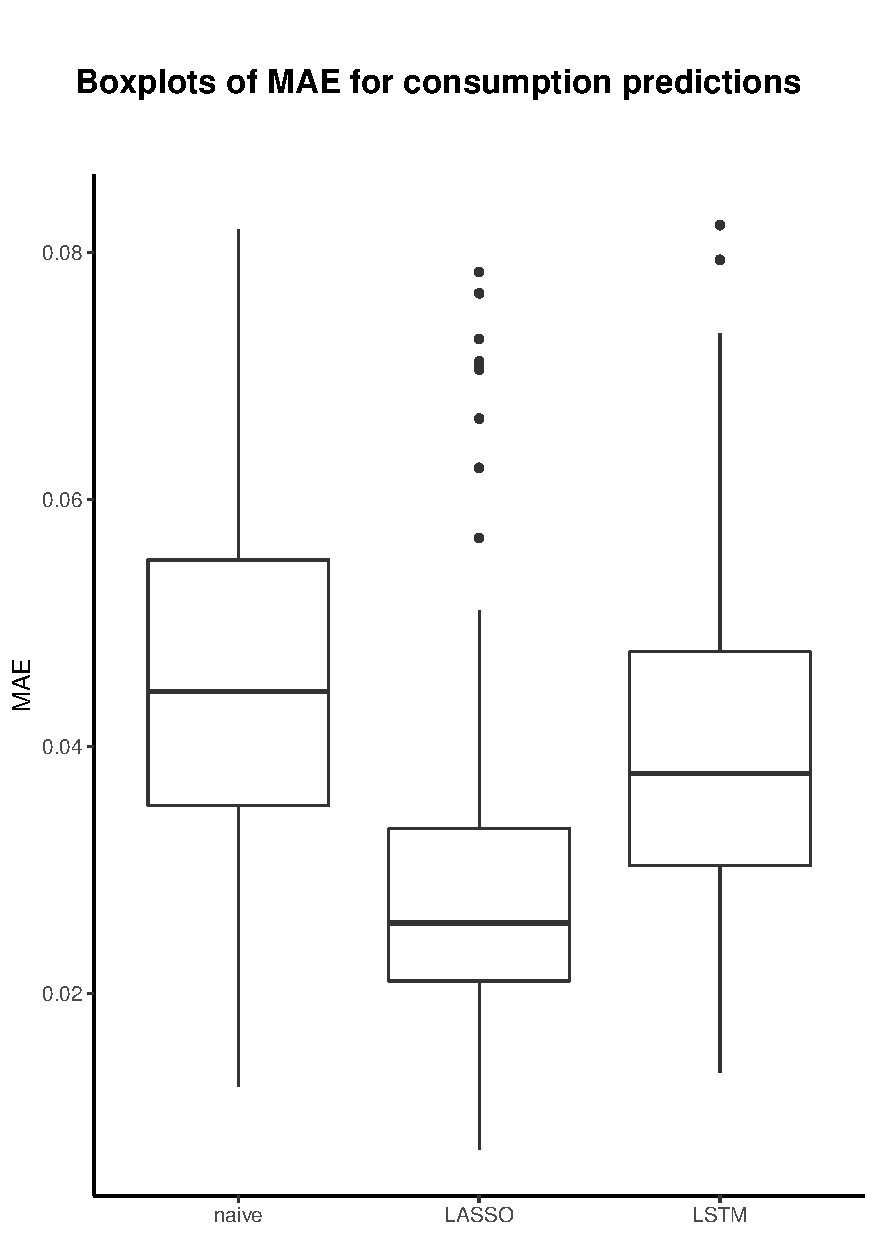
\includegraphics[width=.5\textwidth-5pt]{thesis/graphs/evaluation/c_boxplot_MAE.pdf}
    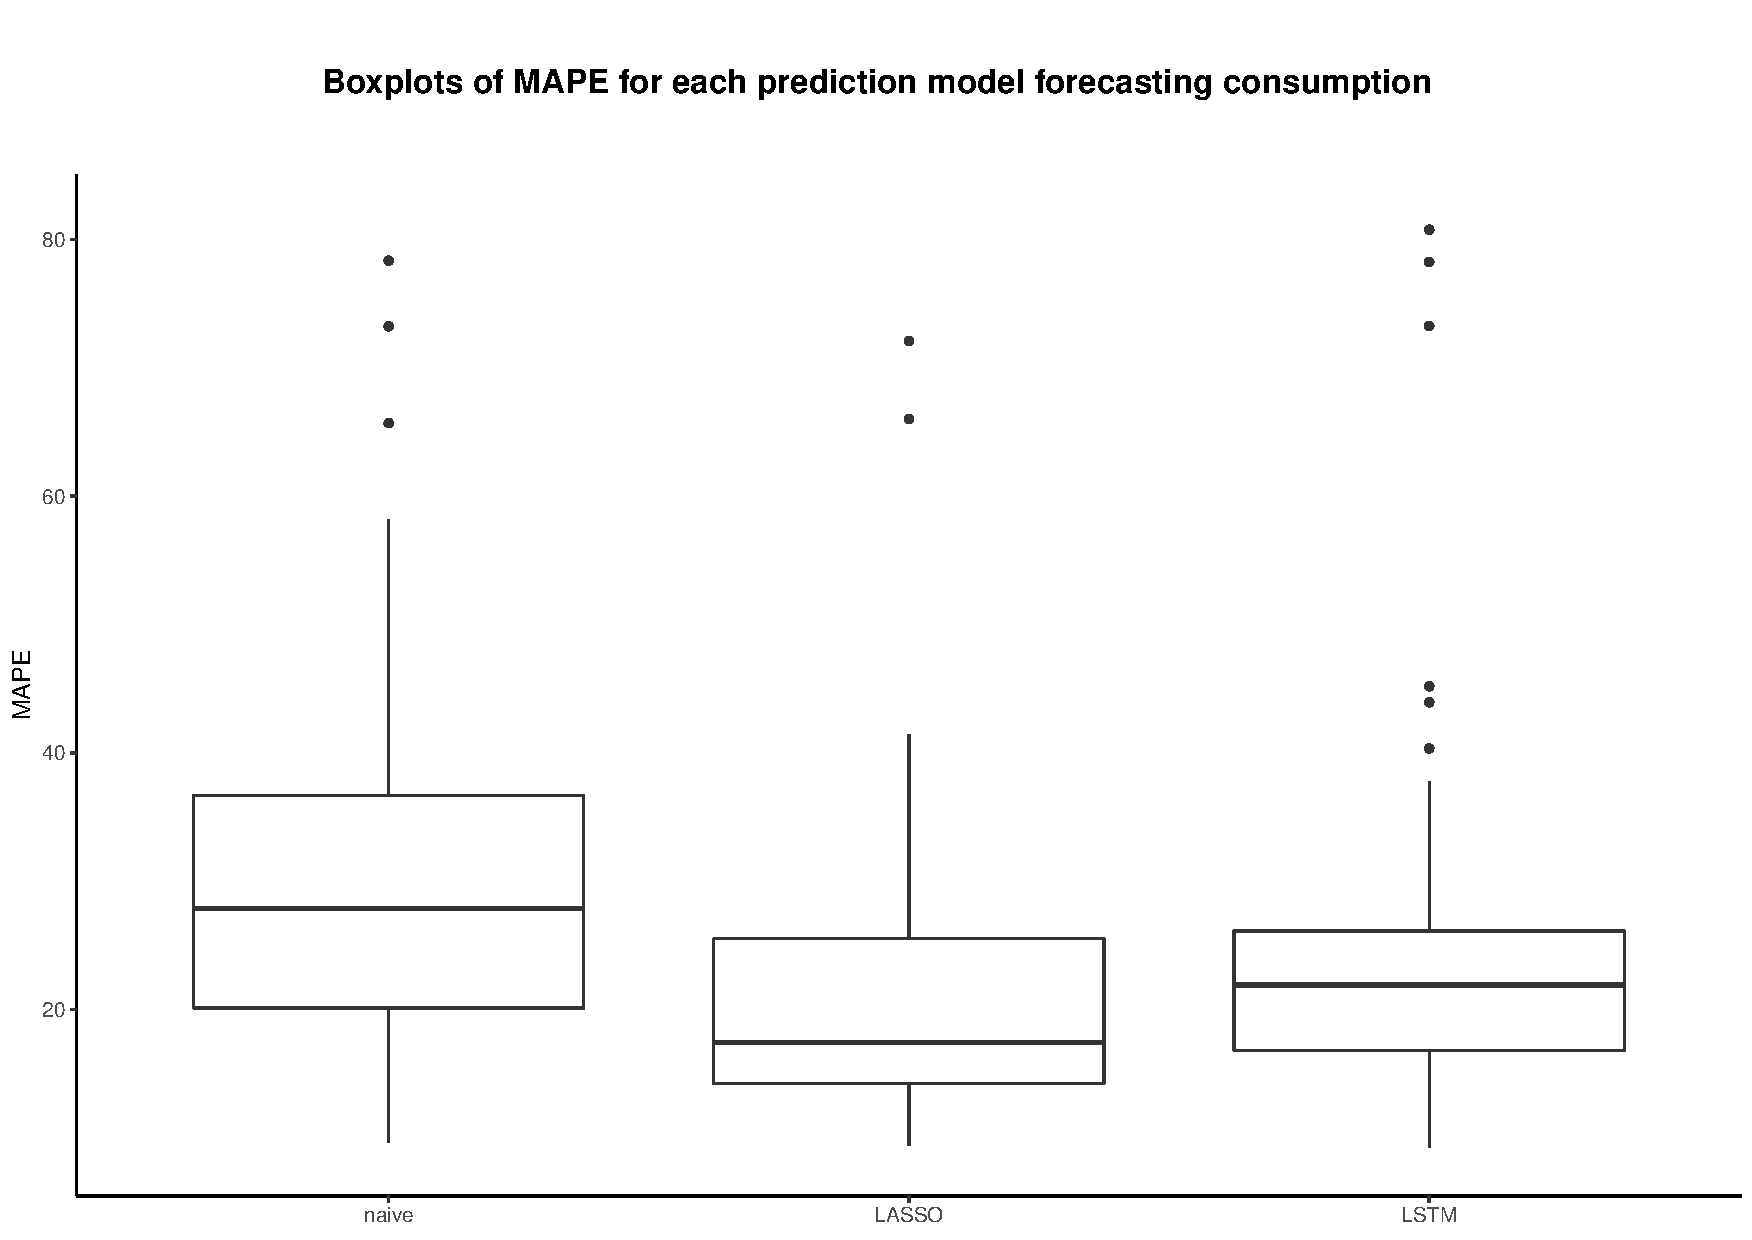
\includegraphics[width=.5\textwidth-5pt]{thesis/graphs/evaluation/c_boxplot_MAPE.pdf} \\
    
    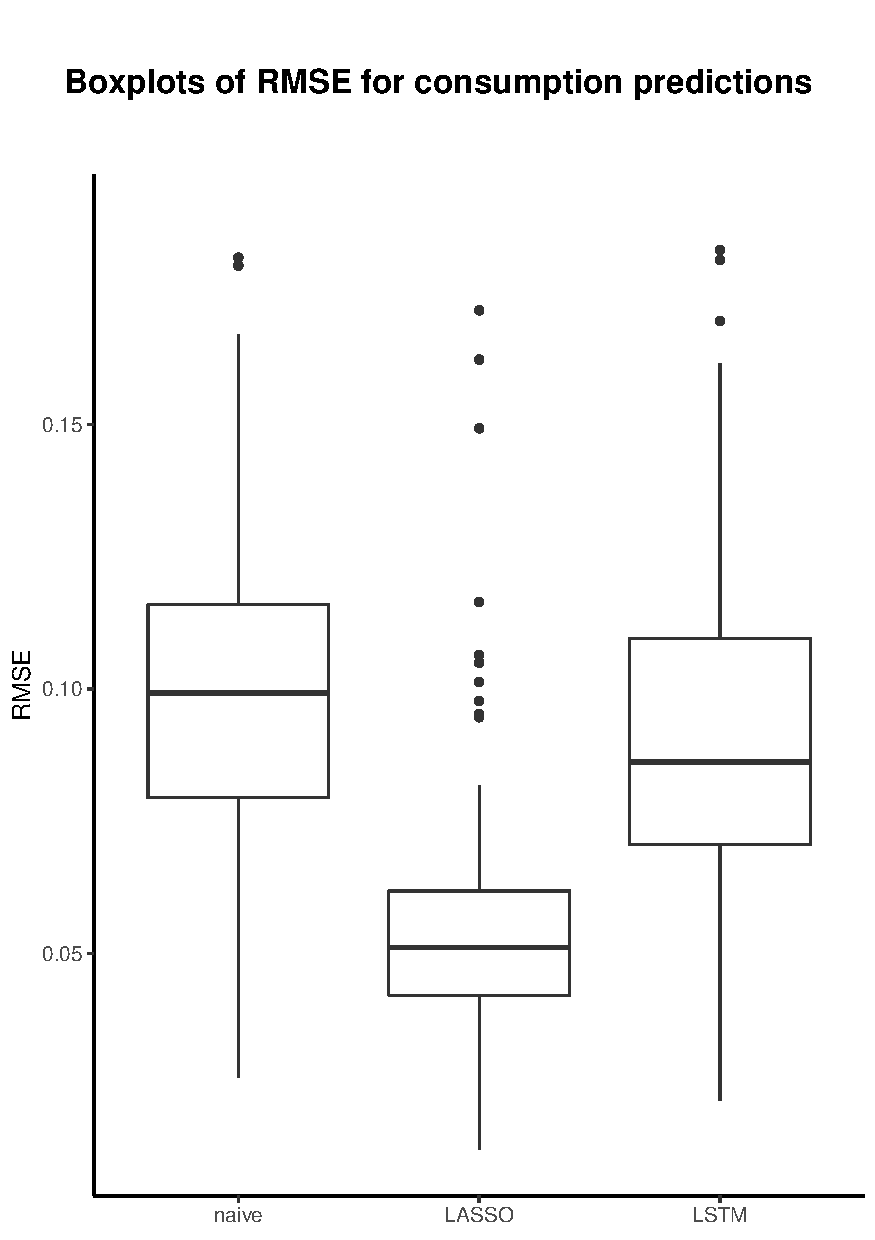
\includegraphics[width=.5\textwidth-5pt]{thesis/graphs/evaluation/c_boxplot_RMSE.pdf}
    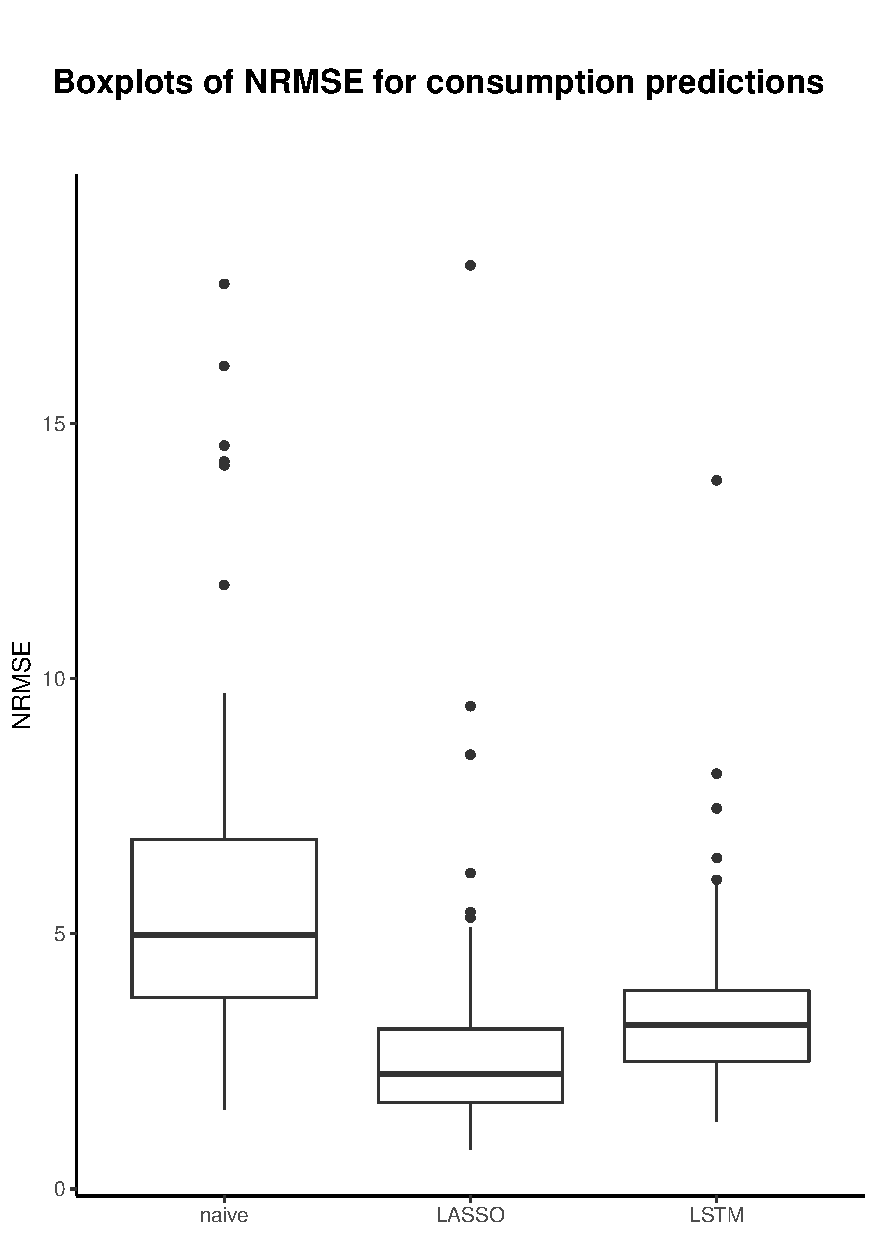
\includegraphics[width=.5\textwidth-5pt]{thesis/graphs/evaluation/c_boxplot_NRMSE.pdf} \\
    \caption[Boxplots of MAE, MAPE, RMSE, and NRMSE scores across consumer data sets]{Boxplots of MAE, MAPE, RMSE, and NRMSE scores across 82 consumer data sets for the three different prediction models (the upper 3 \%-quantile of the error measures is cut off for better readability). \quantnet\href{}{}}
    \label{Fig:boxplots_errormeasures}
\end{figure}
%

Interestingly, there are some consumer data sets with apparently much harder to predict consumption patterns than the other data sets which becomes visible by the outliers of the MAPE and NRMSE boxplots but also by the heatmaps displayed in Figure~\ref{Fig:heatmaps}. Unfortunately, the heatmaps of the relative error measures MAPE and NRMSE are dominated by the very high values for consumer 027. An alternative way to calculate those error measures according to \citet{Hyndman:2006} to avoid very skewed NRMSE or MAPE distribution in the presence of values close to zero is to use the median instead of the mean error. Thus, the mean absolute percentage error becomes the median absolute percentage error (MdAPE) and the normalized root mean squared error becomes the normalized root median squared error (NRMdSE). Taking consumer 027 as an example, the difference becomes clear: The normalized root mean squared error is $\text{NRMSE}_{c027}=2383.46$, while the normalized root \emph{median} squared error is only $\text{NRMdSE}_{c027}=33.43$ (which is still comparatively high). The same holds true for MAPE and MdAPE\footnote{The average MdAPE and NRMdSE across all consumer data sets in comparison to MAPE and NRMSE are presented in Appendix~\hyperlink{AppB2:Tables:avg_errM_wMedian}{B2}.}. Accordingly, the heatmaps for MdAPE and NRMdSE are shown in Figure~\ref{Fig:heatmaps_median}. They confirm that there is a wide variation in the performance of the same prediction methods on the same kind of data but from different households. Therefore, apparently, there is no ``one-size-fits-all'' approach for households' very short-term energy consumption forecasting. Nevertheless, the LASSO model performed best overall. Hence, the predictions on the last quarter of the data produced by the fitted LASSO model for each consumer data set will be used for the evaluation of the market simulation.
%
\begin{figure}[htbp]
 \centering
 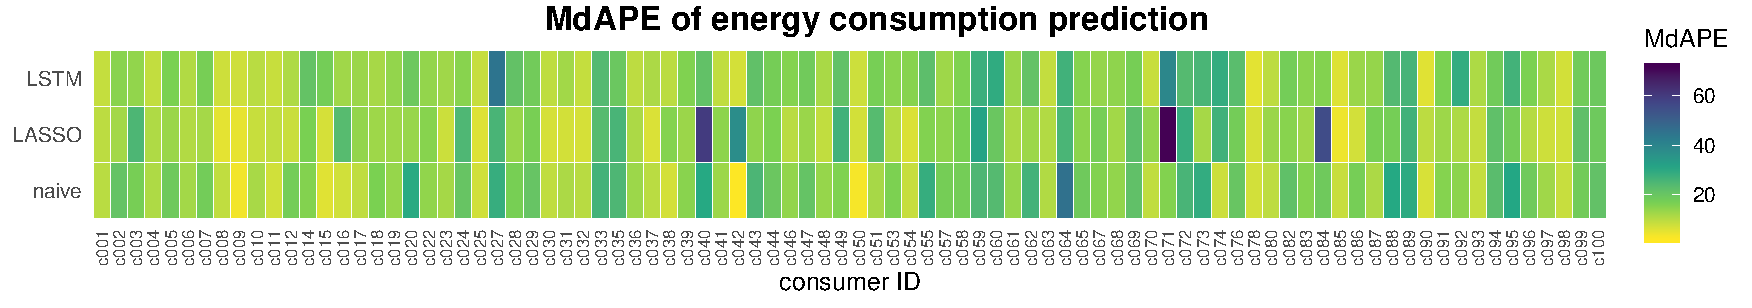
\includegraphics[width=\textwidth]{thesis/graphs/evaluation/c_heatmap_MdAPE.pdf}
 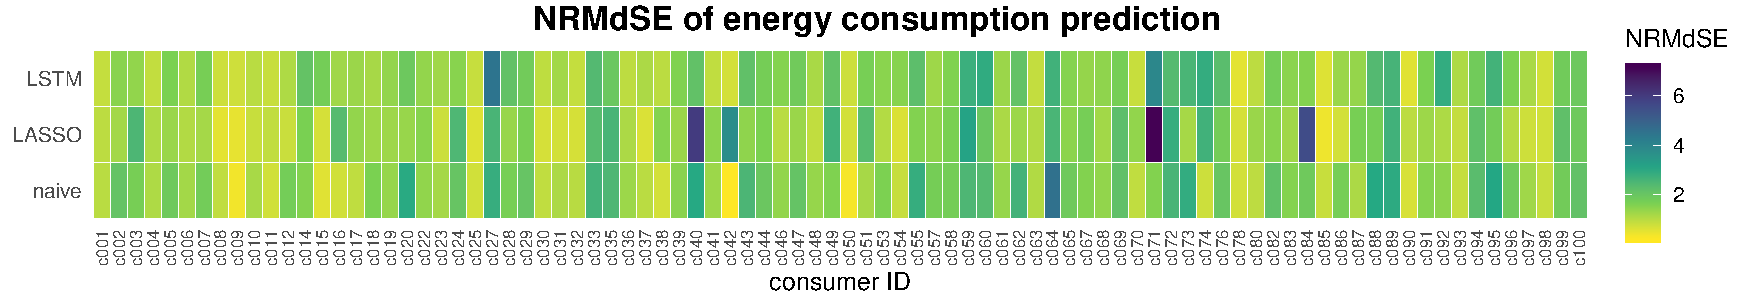
\includegraphics[width=\textwidth]{thesis/graphs/evaluation/c_heatmap_NRMdSE.pdf}
\caption[Heatmaps of MdAPE and NRMdSE for consumption values]{Heatmap of MdAPE and NRMdSE scores for the prediction of consumption values per consumer data set. \quantnet\href{ }{}}
\label{Fig:heatmaps_median}
\end{figure}
%

%%%%%%%%%%%
\subsubsection{Production data}

The performance of the prediction models was tested on a quarter of the available data. That is, the prediction models were fitted on the production values from 01.01.2017~00:00 to 30.09.2017 00:00 which is equivalent to 131,040 data points per data set. For all 12 prosumer data sets, the models were fitted separately resulting in as many distinct LASSO and LSTM prediction models. The fitted models were then used to make energy production predictions in 15-minute intervals for each household individually on the data from 01.10.2017~00:00 to 01.01.2018~00:00. This equates to 8,836 predicted values per data set per prediction method.

Figure~\ref{Fig:glimpse_predprod} exemplary shows the true and predicted production values of prosumer 024 on December 23, 2017. The naive benchmark model just follows the true production shifted by one time step (i.e. 15 minutes). As in the consumption predictions, this fits the true values generally good, as long as there are no sudden jumps in the household's energy production. Jumps or sudden drops in energy production, as in this example one occurred in the 15 minutes before 06:00, necessarily lead to a period with high error of the naive predictor. In such situations, the LASSO model seems more accurate. Even though, it underestimates the jump in energy production, it does not lag behind as much as the naive predictor and, generally, has the ability to anticipate movements. The LSTM-based predictions, on the contrary, fit even worse than the naive predictor in this example. It follows small movements in the energy production time series almost not at all and lags behind the true values similarly to the naive predictor. Also, the LSTM model overestimates constantly in periods of zero production and does not follow at all the upward spike in energy production present in this exemplary snippet of the data.
%
\begin{figure}[htbp]
    \centering
    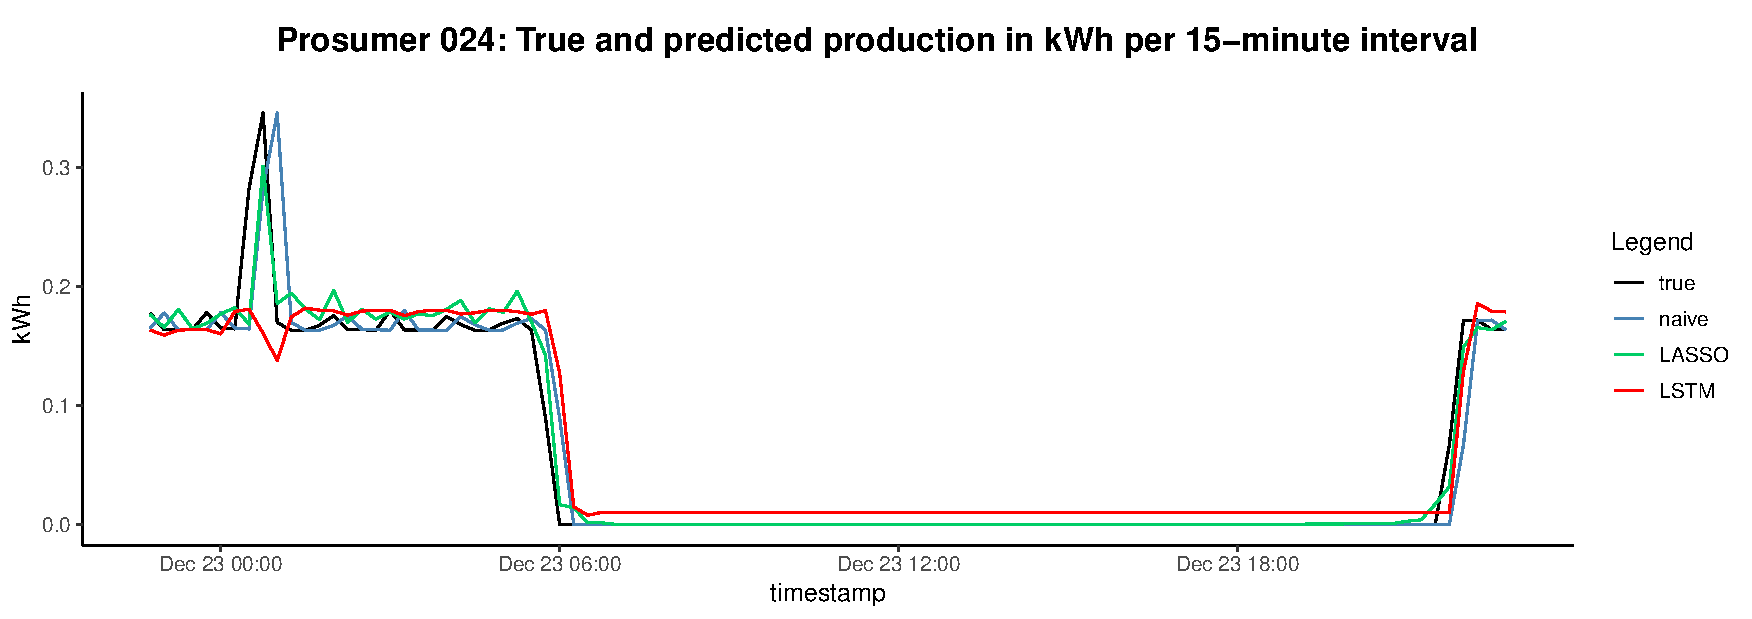
\includegraphics[width=\textwidth]{thesis/graphs/evaluation/p024_pred_prod.pdf}
    \caption[Exemplary 24 hours of true and predicted production values]{Exemplary 24 hours of true and predicted production values of prosumer 024. \quantnet\href{}{}}
    \label{Fig:glimpse_predprod}
\end{figure}
%

Analyzing the over- and underestimation errors of each prediction method on each producer data sets shows the extreme tendency of the LSTM model to underestimate the production values. The LSTM's sum of underestimation errors is substantially larger for six out of twelve prosumer data sets and the sum of overestimation is substantially larger for one data set compared to the LASSO and benchmark model. This already indicates a much worse performance of LSTM on the production data.
%
\begin{figure}
    \centering
    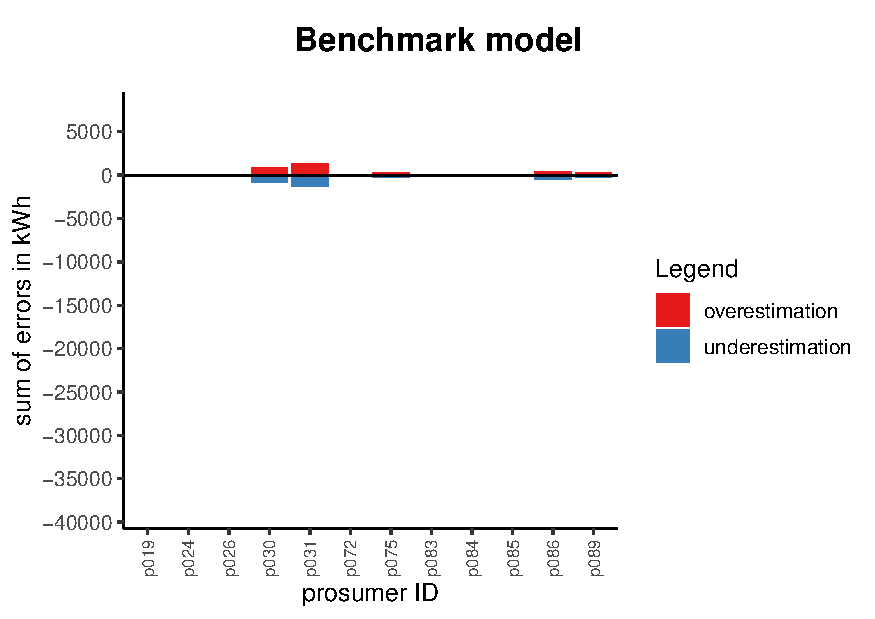
\includegraphics[width=.5\textwidth]{thesis/graphs/evaluation/p_barplot_naive_overunderestimation.pdf}\\\vspace{.6cm}
    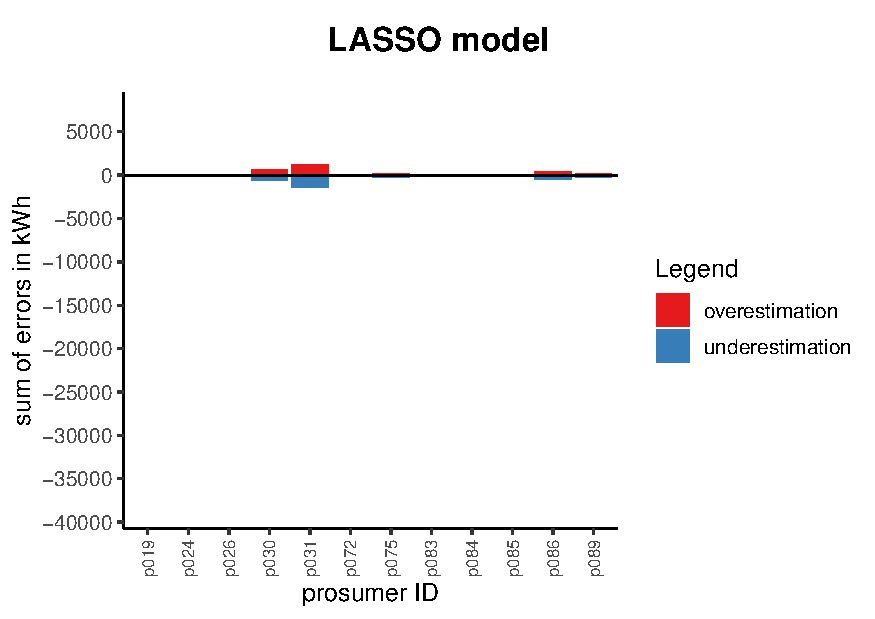
\includegraphics[width=.5\textwidth]{thesis/graphs/evaluation/p_barplot_LASSO_overunderestimation.pdf}\\\vspace{.6cm}
    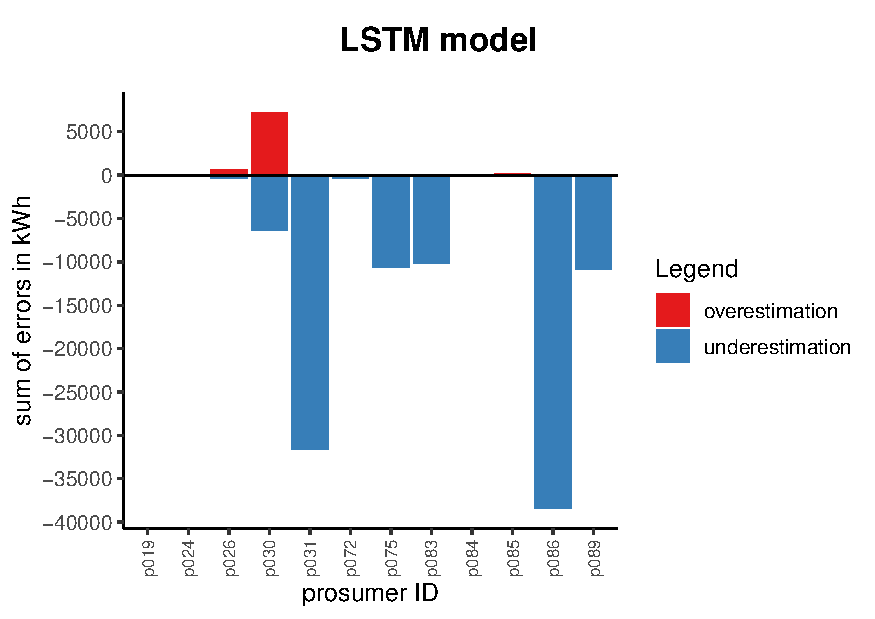
\includegraphics[width=.5\textwidth]{thesis/graphs/evaluation/p_barplot_LSTM_overunderestimation.pdf}
    \caption[Sum of total over- and underestimation errors per prosumer data set]{Sum of total over- and underestimation errors of energy production per prosumer data set and prediction model. \quantnet\href{}{}}
    \label{Fig:overunderestimation_p}
\end{figure}
%

The first impression is confirmed by the average of the error measures across the 12 prosumer data sets shown in Table~\ref{Tab:avg_errormeasures_p}. The LSTM model performs on average much worse than the LASSO and the benchmark model according to MAE, RMSE, and MASE\footnote{Computing the median across the 12 prosumer data sets gives the same qualitative results, although the performance differences are not as extreme (see Appendix~\hyperlink{AppB3:Tables:medain_errM_prod}{B3}).}. MAPE and NRMSE cannot be computed as all production time series contain zero values. As can be seen in Equation~\ref{Eq:MAPE} and Equation~\ref{Eq:NRMSE}, MAPE and NRMSE are not defined if the true value $x_t$ equals zero which is why they cannot be computed for the predictions on production data.
%
\begingroup\catcode`"=9
\begin{table}[ht]
{\footnotesize
    \csvreader[centered tabular=l|SSS,
    before reading=\sisetup{round-mode=places,round-precision=2,round-integer-to-decimal},
    filter not strcmp={\thecsvinputline}{1},
    table head=
    \hline\hline
     \multicolumn{1} {l}{\textbf{Model}} & \multicolumn{1} {c}{\textbf{MAE}} & \multicolumn{1} {c}{\textbf{RMSE}} & \multicolumn{1} {c}{\textbf{MASE}}\\
    \hline,
    no head,
    separator=comma,
    respect all,
    late after line=\\,
    table foot=\hline \hline]
    {thesis/tables/avg_errorMeasures_p.csv}{}%
    {\csvcolii & \csvcoliii & \csvcoliv & \csvcolv}}%
    \caption[Average of error measures for all 12 prosumer data sets]{Average of error measures for the prediction of energy production across all 12 prosumer data sets. \quantnet\href{ }{}}
    \label{Tab:avg_errormeasures_p}
\end{table}
\endgroup
%

%
\begingroup\catcode`"=9
\begin{table}[ht]
{\footnotesize
    \csvreader[centered tabular=l|SSS,
    before reading=\sisetup{round-mode=places,round-precision=2,round-integer-to-decimal},
    filter not strcmp={\thecsvinputline}{1},
    table head=
    \hline\hline
     \multicolumn{1} {l}{\textbf{Model}} & \multicolumn{1} {c}{\textbf{MAE}} & \multicolumn{1} {c}{\textbf{RMSE}} & \multicolumn{1} {c}{\textbf{MASE}}\\
    \hline,
    no head,
    separator=comma,
    respect all,
    late after line=\\,
    table foot=\hline \hline]
    {thesis/tables/avg_errorMeasures_p.csv}{}%
    {\csvcolii & \csvcoliii & \csvcoliv & \csvcolv}}%
    \caption[Average of error measures for all 12 prosumer data sets]{Average of error measures for the prediction of energy production across all 12 prosumer data sets. \quantnet\href{ }{}}
    \label{Tab:avg_errormeasures_p}
\end{table}
\endgroup
%
Overall, it becomes clear that the chosen prediction methods do not forecast energy production of the given prosumer data sets very well. In the case of the LSTM model, this may be due to the hyperparameter tuning being performed on a consumer data set. Moreover, the production data contains much more jumps and discontinuities than the consumption data, which aggravates the prediction task. Due to the unsatisfying performance of the prediction methods on the production data, only the predicted consumption values and the true production values will be used for the market simulation.


%%%%%%%%%%%%%%%%%%%%%%%%%%%%%
%%%   Market simulation   %%%
%%%%%%%%%%%%%%%%%%%%%%%%%%%%%

\subsection{Evaluation of the market simulation}\label{Sec:Results;Subsec:Simulation}

The market simulation used the market mechanism implemented by \citet{Mengelkamp:2018a} in a smart contract to assess the impact of prediction errors on market outcomes. The data sets used for this comprised 88 consumers and 12 prosumers. To evaluate different supply scenario, the market simulation was conducted three times with varying prosumers included. The three scenarios consisted of a market simulation with balanced energy supply and demand, a simulation with severe oversupply and a simulation with severe undersupply. To avoid extreme and unusual market outcomes over the time period of the simulation, two prosumers (prosumer 031 and 086) with high production levels, but long periods of no energy production in the simulation period where not included as energy supplier in the market simulation (see Appendix~\hyperlink{AppA5:Figures:producer_all}{A5}). The remaining prosumers were in- or excluded according to the desired supply scenario. That is, the under supply scenario comprised prosumer 019, 024, 026, 072, 075, and 089, the balanced supply scenario additionally included prosumer 030, and the oversupply scenario additionally included prosumer 083 and 084.

%%%%%%%%%%%
\subsubsection{Market outcomes in different supply scenarios}

The difference between supply and demand for each trading period, the equilibrium price of each closed double auction, and the weighted average price -- called local energy market (LEM) price) -- is shown in Figure~\ref{Fig:marketoutcomes_true_balanced}. The LEM price is computed each trading period as the average of the auctions equilibrium price and the energy utilities energy price (28.69 EURct) weighted by the amount of kWh bought for the respective price. Therefore, in any trading period with higher demand than supply, the LEM price will be above the equilibrium price as the equilibrium price's upper limit is the utilities energy price of 28.69 $\frac{\text{EURct}}{\text{kWh}}$. All graphs depicting the market outcome shown in this section are results of the market simulation with true consumption values. The equivalent graphs for the market simulation with energy consumption values predicted by a LASSO model are shown in Appendix~\hyperlink{AppA6:Figures:marketsimulation_pred}{A6}. As the graphs contain only over-/undersupply and market prices, they are not majorly different when simulating the market mechanism with predicted consumption values (as long as the prediction accuracy is reasonably good). This is not the case for the energy cost that consumers have to bear, as is shown in the next section.

As can be seen, the equilibrium price shown in the middle panel of Figure~\ref{Fig:marketoutcomes_true_balanced} moves roughly synchronous to the over-/undersupply shown in the upper panel. As there is by tendency more undersupply in the balanced scenario, the equilibrium price is in most trading periods close to its upper limit and the LEM price is almost always above the equilibrium price\footnote{Due to the fact, that four of the relevant prosumer data sets contained very large scale producers ($>$10 kWh per 15-minute interval) which dominated the remaining prosumers' production capacity substantially, it was not possible to construct a prosumer sample that better matched the market demand in the balanced supply scenario.}.
%
\begin{figure}[htbp]
    \centering
    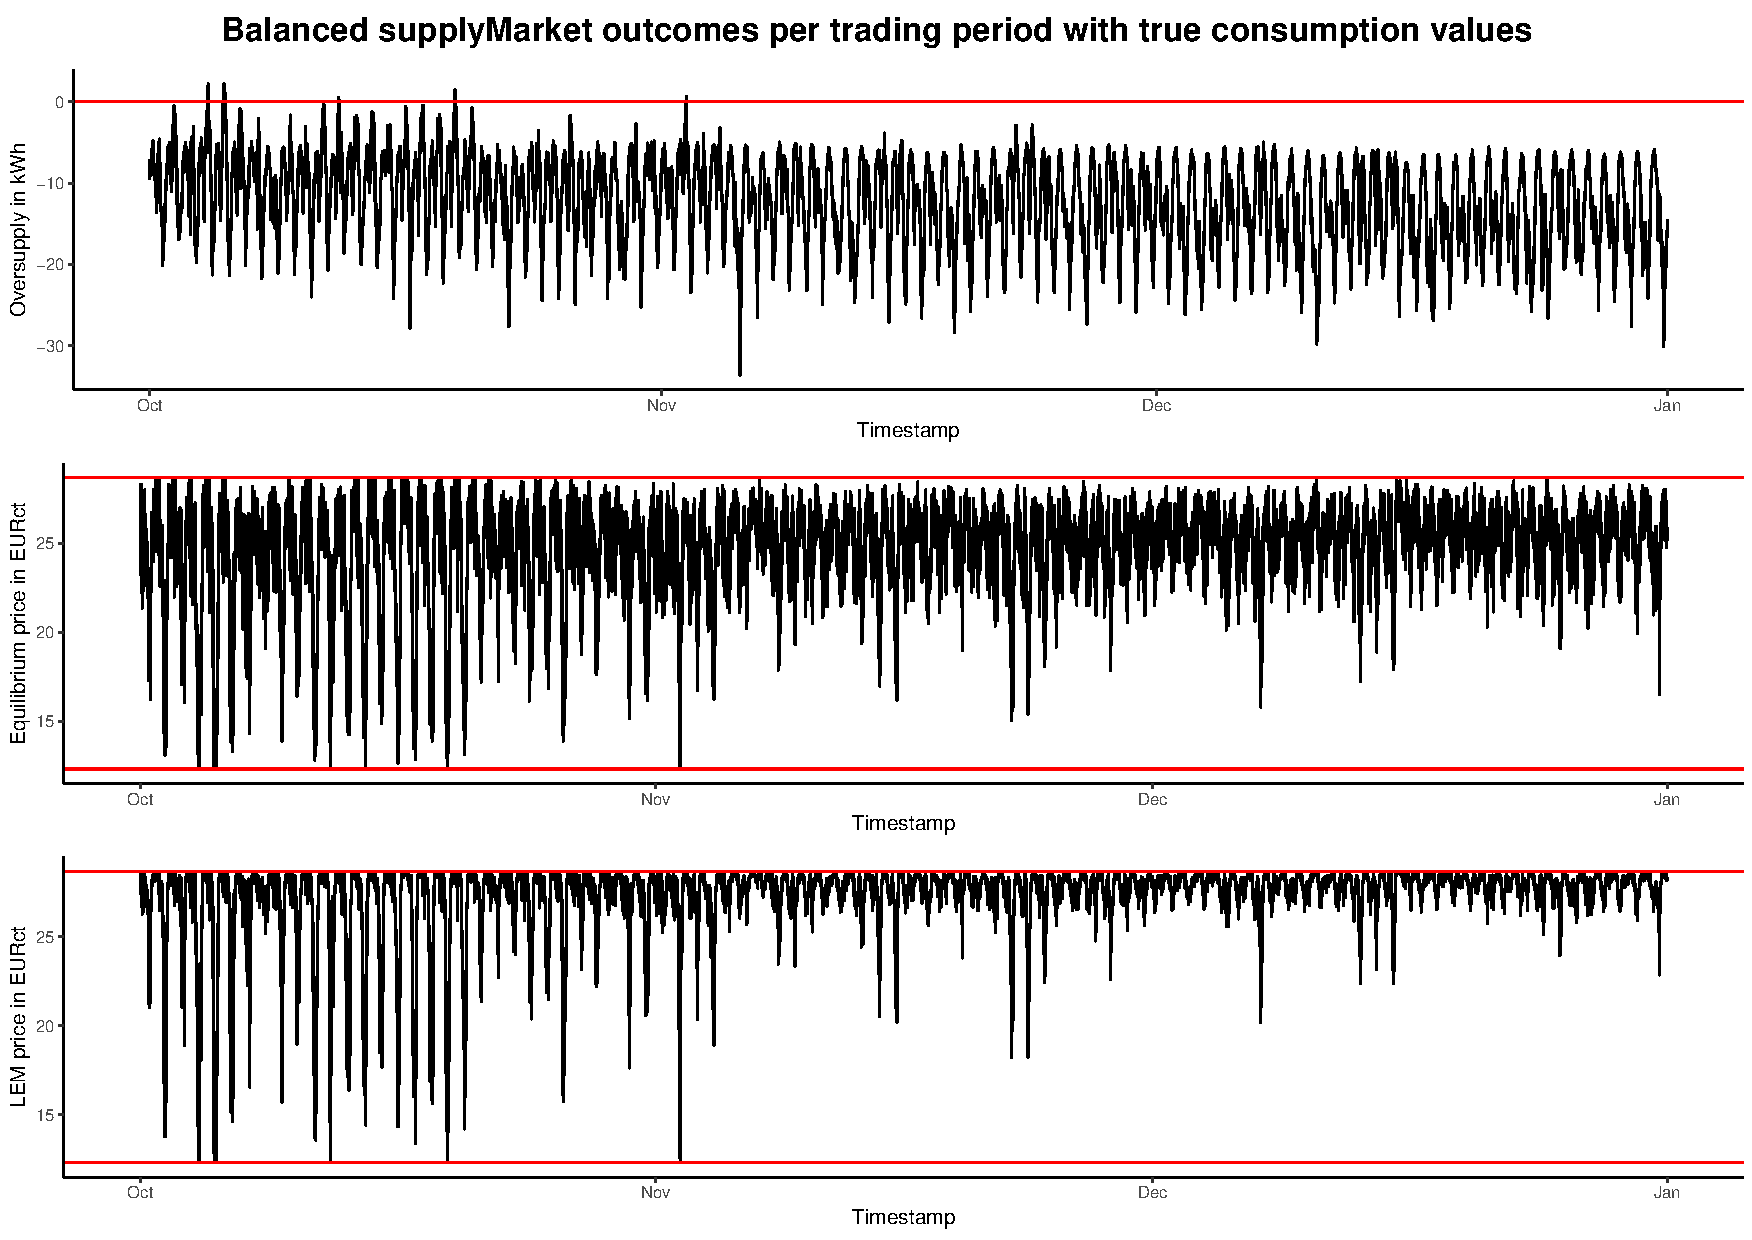
\includegraphics[width=\textwidth]{thesis/graphs/marketsimulation/marketoutcome_true.pdf}
    \caption[Market outcomes simulated with balanced supply and true values]{Market outcomes per trading period simulated with true values and a balanced supply scenario. \quantnet\href{}{}}
    \label{Fig:marketoutcomes_true_balanced}
\end{figure}
%

This is very much contrasted by the oversupply scenario. Here, the prosumers' energy supply surpasses the consumers' energy demand in the majority of trading periods. Accordingly, the equilibrium price in each auction is close to the lower limit of the energy utility's feed-in tariff of 12.31 $\frac{\text{EURct}}{\text{kWh}}$. Still, trading periods with undersupply lead to visible spikes in the equilibrium price which are, as expected, even more pronounced in the LEM price. In all other periods, the equilibrium price equals the LEM price as all demand is served by the prosumers and there is no energy purchased from the grid.
%
\begin{figure}[htbp]
    \centering
    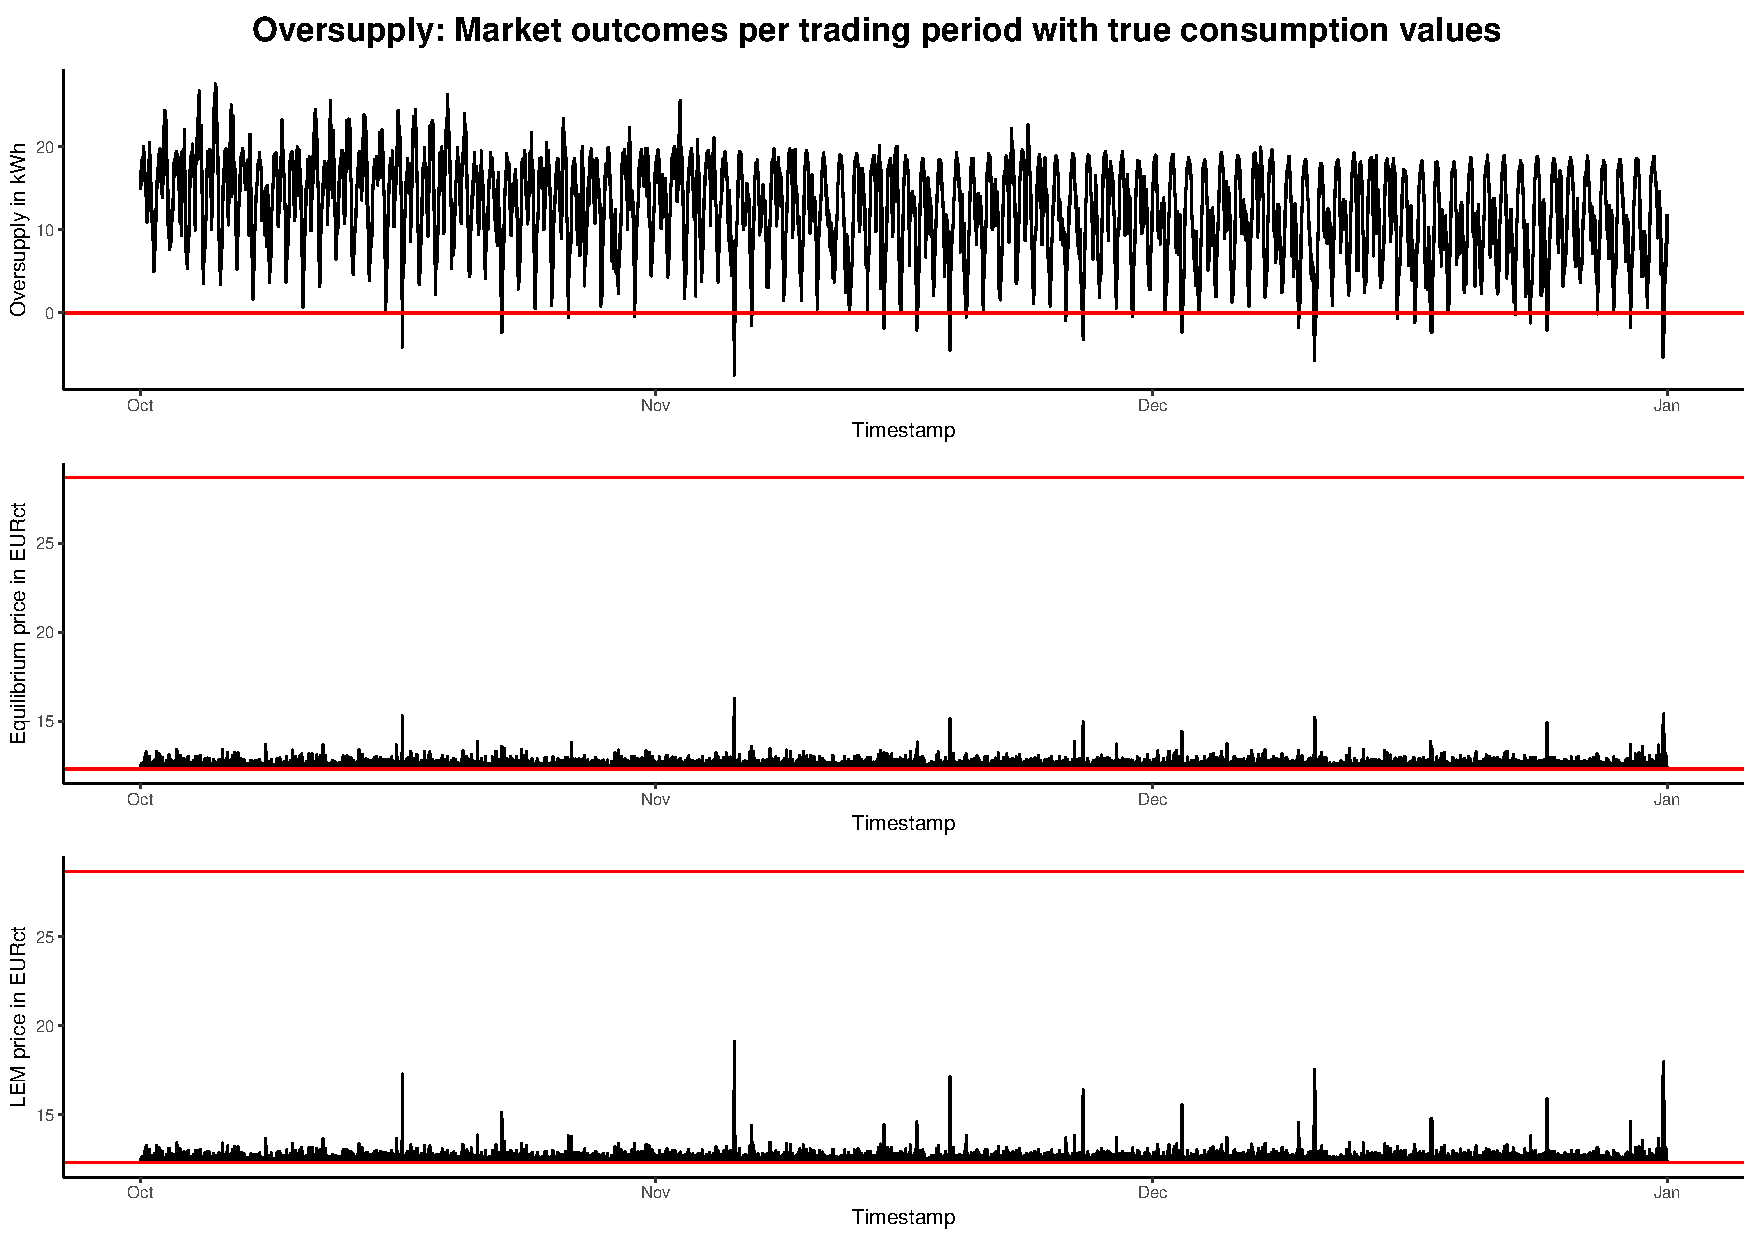
\includegraphics[width=\textwidth]{thesis/graphs/marketsimulation/marketoutcome_true_oversupply.pdf}
    \caption[Market outcomes simulated with oversupply and true values]{Market outcomes per trading period simulated with true values and an oversupply scenario. \quantnet\href{}{}}
    \label{Fig:marketoutcomes_true_over}
\end{figure}
%

The last market simulation is performed with a undersupply scenario. In this case, meeting expectations, the market outcomes are the opposite to the oversupply scenario. The equilibrium prices move in a band between 20 $\frac{\text{EURct}}{\text{kWh}}$ and the upper limit of 28.69 $\frac{\text{EURct}}{\text{kWh}}$. The LEM prices are higher in each period as the deficit in supply has to be compensated by energy purchases from the grid. Therefore, the more severe the undersupply, the more energy has to be purchased from the grid, and the higher is the LEM price above the equilibrium price.
%
\begin{figure}[htbp]
    \centering
    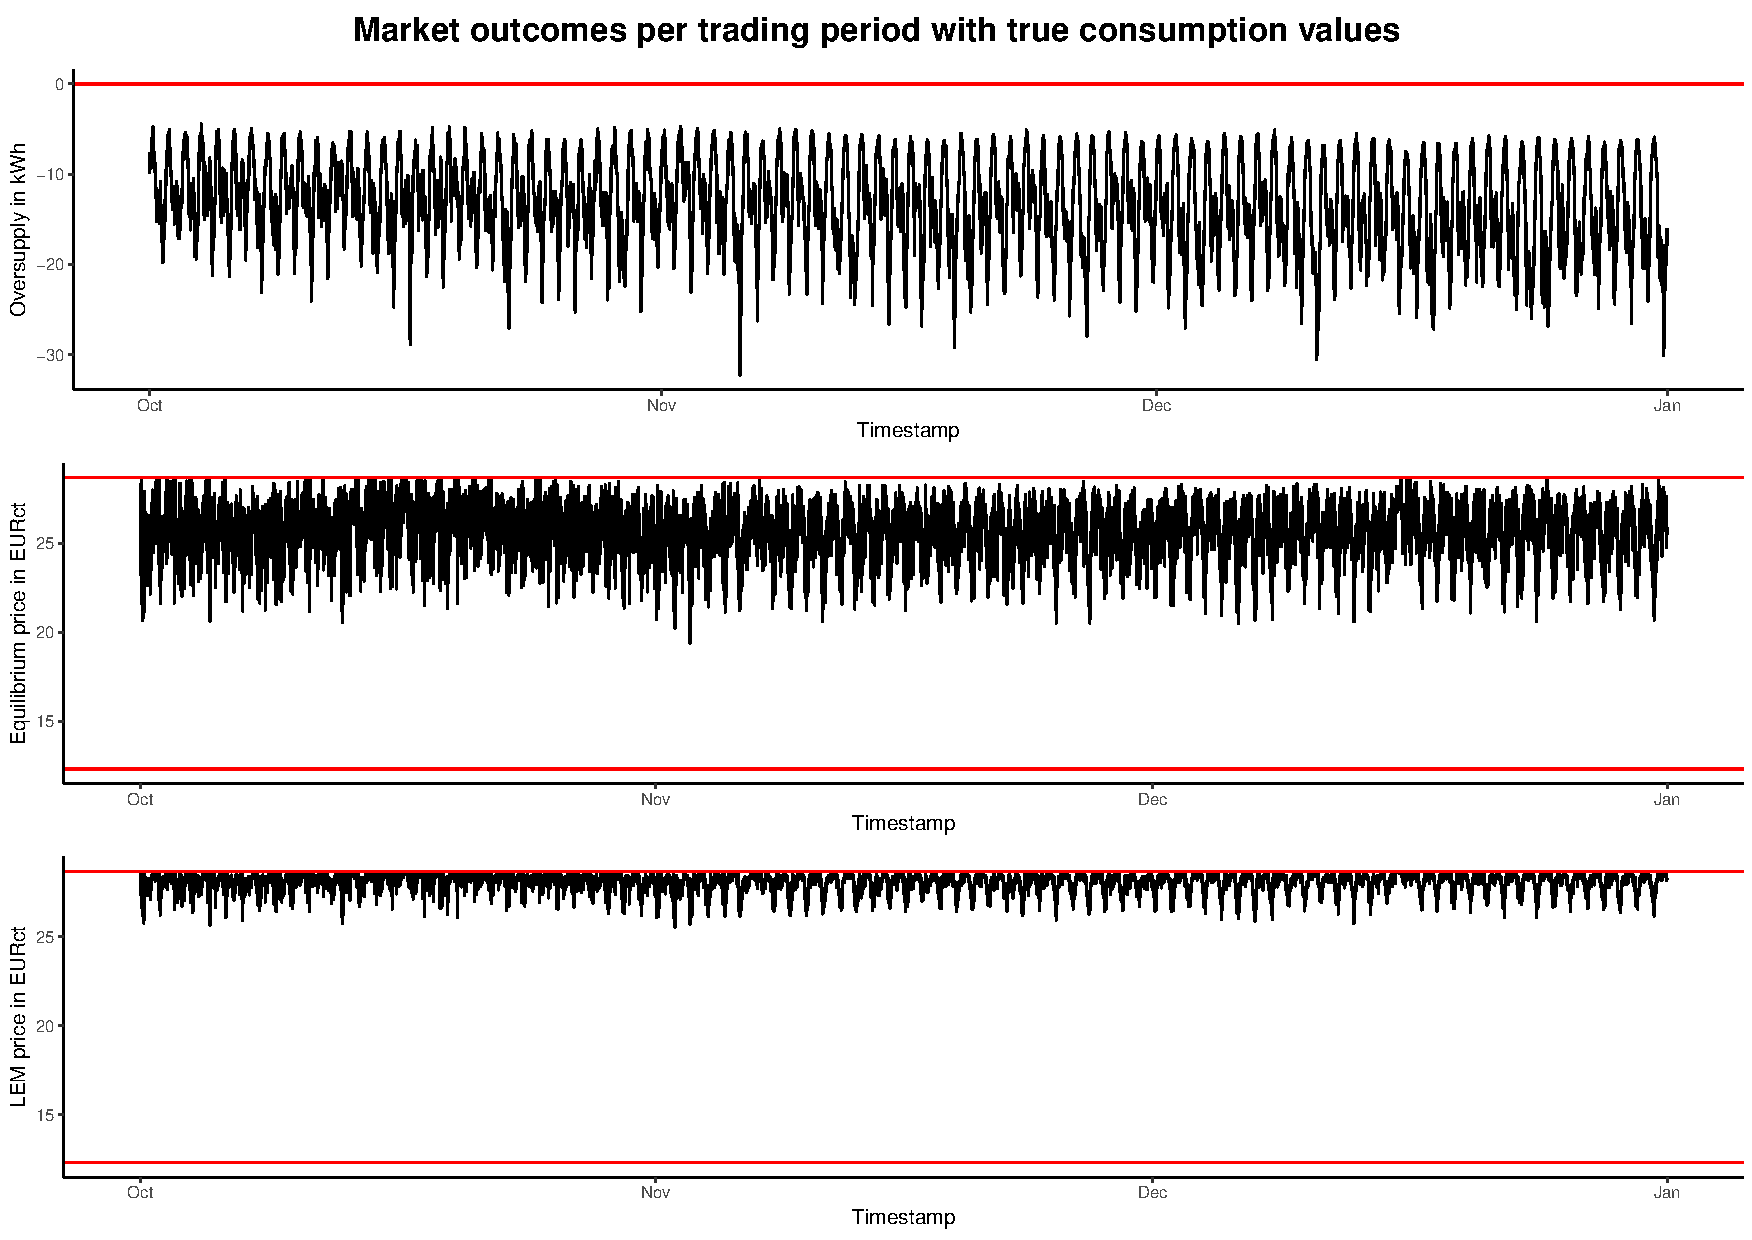
\includegraphics[width=\textwidth]{thesis/graphs/marketsimulation/marketoutcome_true_undersupply.pdf}
    \caption[Market outcomes simulated with undersupply and true values]{Market outcomes per trading period simulated with true values and an undersupply scenario. \quantnet\href{}{}}
    \label{Fig:marketoutcomes_true_under}
\end{figure}
%

In summary, one can conclude that the market outcomes are the more favourable to consumers the more locally produced energy is offered by prosumers. Assuming the specific market mechanism of closed double auctions and the zero-intelligence bidding behaviour of market participants, oversupply reduces the LEM prices substantially leading to savings on the consumer side. On the other hand, prosumers will favor undersupply in the market as they profit from the high equilibrium prices while still being able to sell their surplus energy generation at the feed-in tariff without a loss compared to no LEM. Table~\ref{Tab:simulationresults} summarizes these results.


%%%%%%%%%%%
\subsubsection{Loss to consumers due to prediction errors}

To assess the adverse effect of prediction errors on the market outcomes, the LASSO-predicted energy consumption values per 15 minute interval were used. The prediction of the model served as basis for the auction bids. After the true consumption in the respective trading period was observed, payments to correct over- or underestimation errors were settled. That is, if a consumer bid with a higher amount than actually consumed, it still bought the full bid amount from the prosumers but had to sell the surplus to the energy utility over the grid at the feed-in tariff. On the other hand, if a consumer bid with a lower amount than actually consumed, it bought the bid amount from the prosumers but had to purchase subsequently the surplus energy consumption form the grid at the energy utility's tariff. Thus, prediction errors are costly as the consumer always has to clear the order at less favourable conditions than the equilibrium price provides.

Table~\ref{Tab:simulationresults} contrasts the results of the market simulation in different supply scenario in the case of true and predicted
%
\begingroup\catcode`"=9
\begin{table}[ht]
{\footnotesize
    \csvreader[centered tabular=l|SSSSSS,
    before reading=\sisetup{round-mode=places,round-precision=2,round-integer-to-decimal},
     filter not strcmp={\thecsvinputline}{1},
     %filter expr={
      %test{\ifnumgreater{\thecsvinputline}{2}}},
    table head=
    \hline\hline
     \multirow{2}{2em}{\textbf{Mean}} & \multicolumn{2} {c}{\textbf{Balanced supply}} & \multicolumn{2} {c}{\textbf{Oversupply}} & \multicolumn{2} {c}{\textbf{Undersupply}}\\
     & \multicolumn{1} {c}{\textbf{true}} & \multicolumn{1} {c}{\textbf{predicted}} & \multicolumn{1} {c}{\textbf{true}} & \multicolumn{1} {c}{\textbf{predicted}} & \multicolumn{1} {c}{\textbf{true}} & \multicolumn{1} {c}{\textbf{predicted}}\\
    \hline,
    no head,
    separator=comma,
    respect all,
    late after line=\\,
    table foot=\hline \hline]
    {thesis/tables/average_outcomes.csv}{}%
    {\csvcolii & \csvcoliii & \csvcoliv & \csvcolv & \csvcolvi & \csvcolvii & \csvcolviii}}%
    \caption[Market simulation results for different supply scenarios]{Average results of market simulation for three different supply scenarios. Prices are averaged across all trading periods. Revenues and costs for the whole simulation period are averaged across all prosumers and consumers respectively. \quantnet\href{ }{}}
    \label{Tab:simulationresults}
\end{table}
\endgroup
%

%
\begingroup\catcode`"=9
\begin{table}[ht]
{\footnotesize
    \csvreader[centered tabular=l|SSSSSS,
    before reading=\sisetup{round-mode=places,round-precision=2,round-integer-to-decimal},
    filter not strcmp={\thecsvinputline}{1},
    table head=
    \hline\hline
     \multicolumn{1} {l}{\textbf{Mean}} & \multicolumn{1} {c}{\textbf{Balanced supply}} & \multicolumn{1} {c}{\textbf{Oversupply}} & \multicolumn{1} {c}{\textbf{Undersupply}}\\
    \hline,
    no head,
    separator=comma,
    respect all,
    late after line=\\,
    table foot=\hline \hline]
    {thesis/tables/loss_outcomes.csv}{}%
    {\csvcolii & \csvcoliii & \csvcoliv & \csvcolv}}%
    \caption[Market simulation results for different supply scenarios]{Average results of market simulation for three different supply scenarios. Prices are averaged across all trading periods. Revenues and costs for the whole simulation period are averaged across all prosumers and consumers respectively. \quantnet\href{ }{}}
    \label{Tab:lossresults}
\end{table}
\endgroup
%

%
\begin{figure}[htbp]
    \centering
    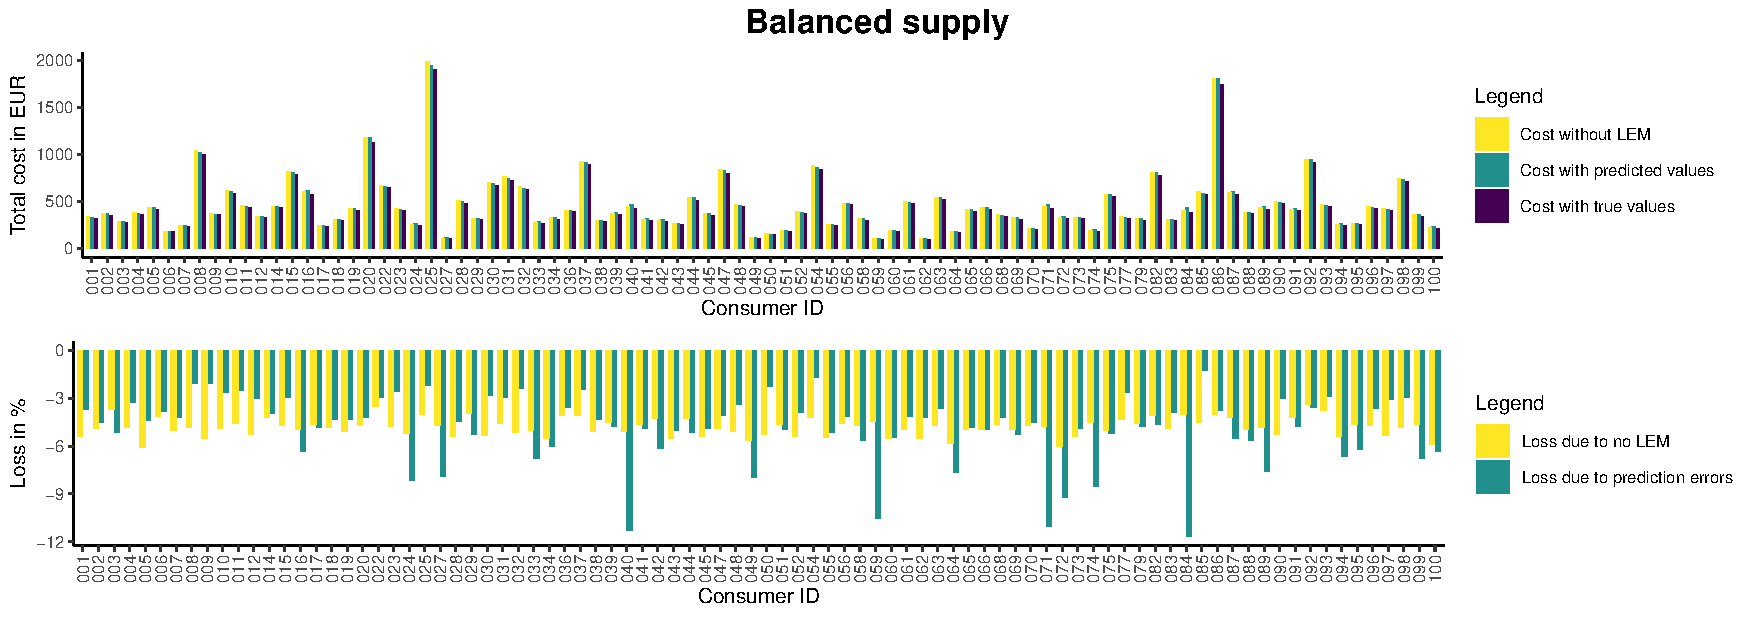
\includegraphics[width=\textwidth]{thesis/graphs/marketsimulation/totalenergycost.pdf}\\\vspace{.6cm}
    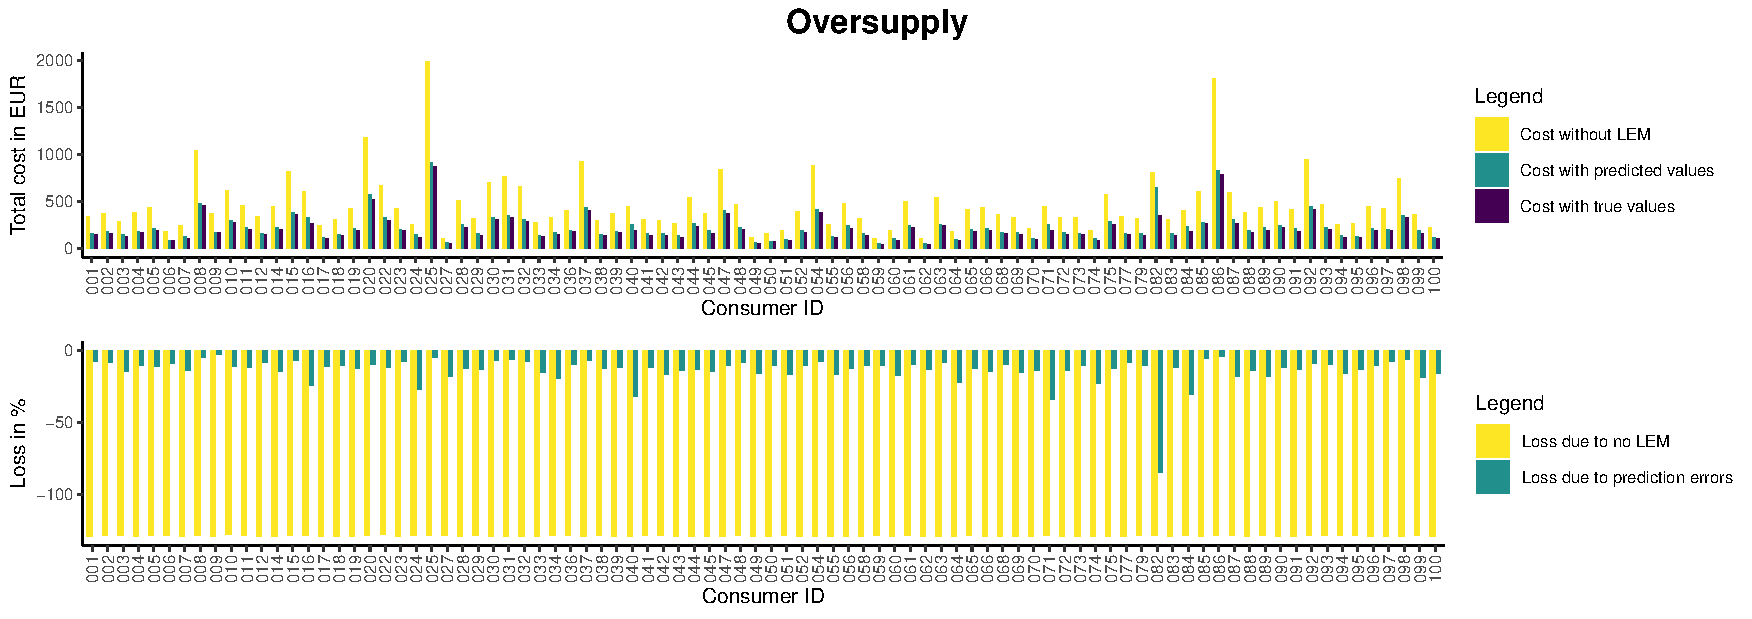
\includegraphics[width=\textwidth]{thesis/graphs/marketsimulation/totalenergycost_oversupply.pdf}\\\vspace{.6cm}
    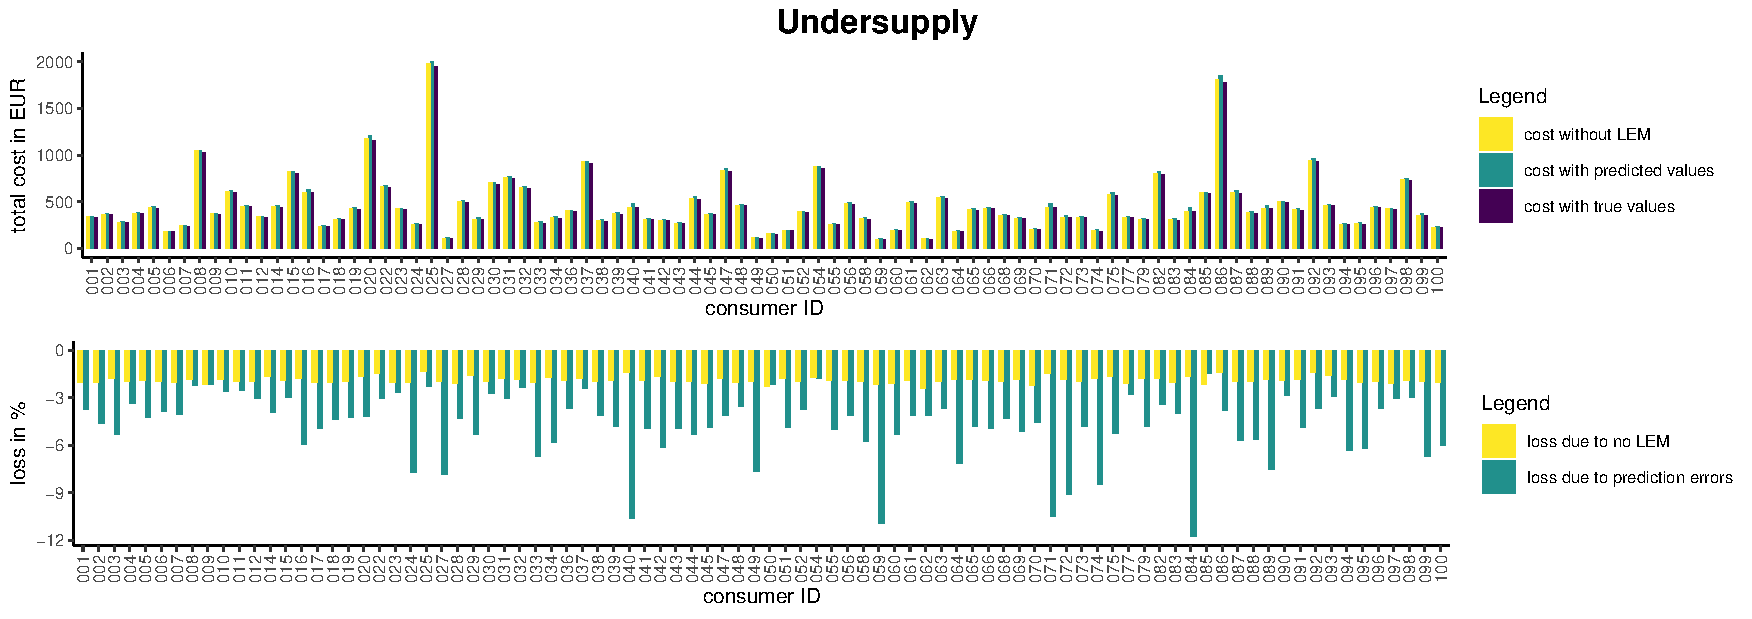
\includegraphics[width=\textwidth]{thesis/graphs/marketsimulation/totalenergycost_undersupply.pdf}
    \caption[Total energy cost to consumers in different supply scenarios]{Total energy cost to consumers from 01.10.2018 to 31.12.2017 in case of no LEM, LEM with true values, and LEM with predicted values in three different supply scenarios. \quantnet\href{}{}}
    \label{Fig:total_energycost}
\end{figure}
%



%%%%%%%%%%%
%\subsubsection{Predicted consumption and true production values}




%%%%%%%%%%%%%%%%%%%%%%%%%%%%%%%%%%%%%%%%%%%%%%%%%%%%%%%%%%%%%%%%%

\begin{itemize}

    \item Organize material and present results.

    \item Use tables, figures (but prefer visual presentation):
        \begin{itemize}
            \item Tables and figures should supplement (and not duplicate) the
                text.

            \item Tables and figures should be provided with
            legends.\\
                {\it Figure~\ref{Fig:Resids} shows how to include and reference
                graphics. The graphic must be labelled before. Files must be in
                \texttt{.eps} format.}

                \begin{figure}[ht]
                \begin{center}
                    \includegraphics[scale=0.5,angle=0]{thesis/figures/graph.pdf}
                    \caption{Estimated residuals from model XXX. ...}
                    \label{Fig:Resids}
                \end{center}
                \end{figure}

            \item Tables and graphics may appear in the text or in
                the appendix, especially if there are many simulation results
                tabulated, but is also depends on the study and number of tables resp.
                figures. The key graphs and tables must appear in
                the text!
        \end{itemize}

    \item Latex is really good at rendering formulas:\\
        {\it Equation (\ref{Eq:SpecDens}) represents the ACs of a stationary
        stochastic process:
        \begin{equation}
            f_y(\lambda) = (2\pi)^{-1} \sum_{j=-\infty}^{\infty}
                           \gamma_j e^{-i\lambda j}
                         =(2\pi)^{-1}\left(\gamma_0 + 2 \sum_{j=1}^{\infty}
        \gamma_j \cos(\lambda j)\right)
                                        \label{Eq:SpecDens}
        \end{equation}
        where $i=\sqrt{-1}$ is the imaginary unit, $\lambda \in [-\pi,
        \pi]$ is the frequency and the $\gamma_j$ are the autocovariances
        of $y_t$.}

\newpage

    \item Discuss results:
        \begin{itemize}
            \item Do the results support or do they contradict economic theory ?
            \item What does the reader learn from the results?
            \item Try to give an intuition for your results.
            \item Provide robustness checks.
            \item Compare to previous research.
        \end{itemize}
\end{itemize}


\section{Conclusion}\label{Sec:Conc}



%%%%%%%%%%%%%%%%%%%
%%%   Summary   %%%
%%%%%%%%%%%%%%%%%%%%

\subsection{Summary of present research}\label{Sec:Conclusion;Subsec:Summary}

The present research aimed to evaluate, first, the prediction accuracy for household energy consumption and production using state-of-the-art forecasting techniques. Second, to assess the effect of prediction errors in a market simulation using the market mechanism implemented by \citet{Mengelkamp:2018a} in a smart contract on a blockchain. And lastly, to infer the implications of the results for the future design of blockchain-based local energy markets.

For this purpose, first, the performance of two forecasting techniques, which were already successfully applied in previous research, was assessed. A LSTM recurring neural network and a LASSO regression model were fitted on 9 months of consumption respectively production data of German households recorded by smart meters in 3-minute intervals. These models were then used to predict energy consumption respectively production in 15-minute resolution one-step ahead for three months. The predictions were evaluated using several error measures and compared to a benchmark model (na\"ive persistence model). The LASSO model yielded the best results with an average MAPE across all consumer data sets of \textapprox17~\% and was subsequently used to make predictions for the succeeding market simulation. As all prediction models failed to produce satisfactory predictions on the production data, the market simulation used only true production values.

Secondly, the market mechanism implemented by \citet{Mengelkamp:2018a} was used to assess the effect of prediction errors on market outcomes in three different supply scenarios. The evaluation revealed that in a balanced supply and demand scenario the settlement cost due to prediction errors almost completely offset savings introduced by the participation in the local energy market. In an undersupply scenario, the cost due to prediction errors even surpassed the savings and made market participation uneconomical. Only in a scenario with substantial oversupply, the savings brought to consumers by the participation in the local energy market compensated the cost of prediction errors completely.

Thus, thirdly, further possible adjustments necessary for future blockchain-based local energy markets to mitigate this finding were discussed. Here, it was found that this problem would be only diminished but not eliminated by more accurate forecasts. Moreover, it seemed unlikely that the performance of prediction models could be greatly improved without including higher data resolution, behavioural variables, and data from smart appliances (as done by \citet{Kong:2018}) -- which still would not compensate for the unpredictability of human behaviour. Implementing blockchain-based LEM only in market setups with oversupply seems impractical and would most probably diminish the advantages of LEM substantially. Therefore, the most promising approach seemed to be measures that address the market design. This mainly includes adjustments to the market mechanism, which can be two-fold: Either shorter trading periods could introduced which in turn reduces the forecasting horizon and therefore prediction errors or the auction mechanism is altered to use actual consumption values to settle transactions.

Overall, the need to take prediction errors into consideration in the design of blockchain-based market mechanism became evident. This is due to the high uncertainty associated with individual households' energy consumption and therefore also net production patterns that limits the feasibility of accurate forecasts substantially.



%%%%%%%%%%%%%%%%%%%%%%
%%%   Discussion   %%%
%%%%%%%%%%%%%%%%%%%%%%

\subsection{Limitations of present research}\label{Sec:Conclusion;Subsec:Discussion}

There are some limitations to point out of the present work. One major point is that data from more smart meters and more context information about the data would have been desirable. Due to data protection legislation no information regarding locality of the households, the household characteristics or the type of power plant prosumer households used could be provided by Discovergy. This made it difficult to judge the suitability of certain data sets for the market simulation and required a detailed analysis of the energy recordings' patterns of every single data set provided. Also the large share of so declared prosumer data sets without any net energy production readings was unfortunate and unexplained. The large scale differences in the production capacities of the remaining prosumers with net energy production readings complicated the analysis of the market simulation further. Additionally, it would have been preferable to have absolute production and consumption data for prosumers instead of the net consumption respectively production. Although, this circumstance reflected data real-world data availability and is something probably every implementation of blockchain-based LEM would have to deal with. This fact, however, highlights the necessity to improve net demand forecasting as has been already pointed out in previous research as well \citep[e.g.,][]{Meer:2018, Hong:2016}.

The prediction performance of the LSTM model was slightly surprising. The author would have expected better results, especially compared to the LASSO regression model. Here, a major constrained for more elaborate model architectures, the inclusion of more data points and more sophisticated and granular hyperparameter tuning was computing resources. The computing resources available were either not optimized for large scale neural network training (i.e., a lack of graphical processing units (GPUs) capable of tensor operations) or prohibitively expensive to use exceeding the free trial credits for computing resources (i.e., the Google Cloud Platform Free Tier). Especially, the predictions on prosumer data sets could have been much better. Here exist dedicated research fields for the forecasting of electricity production by different type of plants. However, this knowledge could not be adequately put to use in the present work as the households' type of production plants was not known or would have had to be inferred from net production patterns with a high degree of uncertainty.

The evaluation of the predictions on production data also suffered from the unavailability of relative error measures due to the frequent occurence of zero values. The usage of MAPE or NRMSE with the plants production capacity as denominator (as suggested by \citet{Hoff:2013}) would have solved this problem, however, would have required knowledge about the maximum capacity which was again not available. Another promising approach to quantify error measures in the presence of sudden unexpected peaks is the ramp score as utilized in wind energy forecasting and developed on the basis of a swinging door algorithm \citep[e.g.,][]{Bianco:2016, Florita:2013}. This may be useful to include in future similar work.

Finally, it is to mention that the market simulation did not account for taxes or fees, especially grid utilization fees which can be a substantial share of the total electricity cost of households. Moreover, the simulation does not take into account compensation costs for blockchain miners that reimburses them for the computational cost the bear. The modeling of this cost and potential distribution schemes among market participants is definitively needed in future research on blockchain-based energy markets \citep{Mengelkamp:2018a}.



%%%%%%%%%%%%%%%%%%%
%%%   Outlook   %%%
%%%%%%%%%%%%%%%%%%%

\subsection{Outlook and further research}\label{Sec:Conclusion;Subsec:Outlook}

Naturally, future research concerned with blockchain-based LEM should take into account the potential cost of prediction errors. This implies a focus on market mechanisms and prediction error settlement structures that do not make participation in the LEM uneconomical. A special focus on this issue has to be put in situations with undersupply of locally produced energy. A further field of research that already is picking up in sophistication and amount is the forecast of individual household energy consumption and production. While the results of this field are still nowhere close to the forecasting accuracy of aggregated consumption forecasting, there is still room for improvement and refinement of existing prediction techniques. Any advancements made in the prediction of individual households' energy patterns also benefits the blockchain-based LEM research as energy forecasts most likely will play a role in their use cases. Furthermore, to the author's knowledge there has been no simulation of blockchain-based LEM with actual consumption and production data conducted. Doing so on a private blockchain with the market mechanism coded in a smart contract should be the next step for the assessment of potential technological and conceptual weaknesses.

Previous research has shown that blockchain technology and smart contracts can play a valuable role in tackling the challenges of a changing energy landscape. This research emphasizes, however, that advancement on this front cannot be made without a holistic approach that takes all components of blockchain-based local energy markets into account. Simply assuming that reasonably accurate energy forecasts for individual households will be available once the technical challenges of implementing a LEM on a blockchain are solved, may steer research into a wrong direction and miss the opportunity to quickly move into the direction of a more sustainable and less carbon-intensive future.


%%%%%%%%%%%%%%%%%%%%%%%%%%%%%%%%%%%%%%%%%%%%%%%%%%%%%%%%%%%%%%%%%



% ----------------
% --- appendix ---
% ----------------
\appendix

% literature
\newpage
\addcontentsline{toc}{section}{References}
\bibliography{thesis/99_literature.bib}

% figures
\newpage

\section{Figures}\label{App:Figures}

\subsection{Excluded consumer data sets}\label{App:Figures:Excludedc}

\begin{centering}
\begin{figure}[!htbp]
        \includegraphics[width=\textwidth-0.85cm]{thesis/graphs/timeseries/c021_cons.pdf}\vspace{0.3cm}
        \includegraphics[width=\textwidth-0.85cm]{thesis/graphs/timeseries/c046_cons.pdf}
\end{figure}
\begin{figure}[!htbp]
        \includegraphics[width=\textwidth-0.85cm]{thesis/graphs/timeseries/c053_cons.pdf}\vspace{0.3cm}
        \includegraphics[width=\textwidth-0.85cm]{thesis/graphs/timeseries/c057_cons.pdf}
\end{figure}
\begin{figure}[!htbp]
        \includegraphics[width=\textwidth-0.85cm]{thesis/graphs/timeseries/c078_cons.pdf}\vspace{0.3cm}
        \includegraphics[width=\textwidth-0.85cm]{thesis/graphs/timeseries/c080_cons.pdf}
        \caption[Consumer data sets excluded due to peculiarities in the consumption patterns]{Consumer data sets excluded due to peculiarities in the consumption patterns. \quantnet}
        \label{App:Fig:excludedcons}
\end{figure}
\end{centering}


\subsection{Excluded consumer data sets}\label{App:Figures:Excludedp}

\begin{centering}
\begin{figure}[!htbp]
        \includegraphics[width=\textwidth-0.85cm]{thesis/graphs/timeseries/p012_prod&cons.pdf}\vspace{0.3cm}
        \includegraphics[width=\textwidth-0.85cm]{thesis/graphs/timeseries/p015_prod&cons.pdf}
        \caption[Consumer data sets excluded due to peculiarities in the consumption patterns]{Consumer data sets excluded due to peculiarities in the consumption patterns. \quantnet}
        \label{App:Fig:excludedpros}
\end{figure}
\end{centering}


%%%%%%%%%%%%%%%%%%%%%%%%%%%%%%%%%%%%%%%%%%%%%%%%%%%%%%%%%%%%

\begin{figure}[ht]
    \begin{center}
        \includegraphics[scale=0.5,angle=0]{thesis/figures/graph.pdf}
        \caption{Estimated residuals (2) from model XXX. ...}
        \label{Fig:Resids2}
    \end{center}
\end{figure}


% tables
\newpage

\section*{Appendix \hypertarget{AppB:Tables}{B}: Tables}\label{App:Tables}

\subsection*{\hypertarget{AppB1:Tables:totalcons}{B1} Summary statistics of total energy consumption and production} \label{AppB1:Tables:totalcons}

\begin{table}[ht]
{\footnotesize
    \csvreader[centered tabular=l|......,
    filter not strcmp ={\thecsvinputline}{1},
    table head=
    \hline\hline
     & \multicolumn{1} {|c}{\textbf{Min}} & \multicolumn{1} {c}{\textbf{Q1}} & \multicolumn{1} {c}{\textbf{Median}} & \multicolumn{1} {c}{\textbf{Mean}} & \multicolumn{1} {c}{\textbf{Q3}} & \multicolumn{1} {c}{\textbf{Max}}\\
    \hline,
    no head,
    separator=comma,
    respect all,
    late after line=\\,
    table foot= \hline \hline]
    {thesis/tables/summarystats_total.csv}{}%
    {\csvcoli & \csvcolii & \csvcoliii & \csvcoliv & \csvcolv & \csvcolvi & \csvcolvii}}%
    \caption[Summary statistics of households' total consumption and production in 2017]{Summary statistics of households' total consumption and production in 2017. \quantnet\href{ }{BLEMdescStatEnergy}}
\end{table}


\subsection*{\hypertarget{AppB2:Tables:avg_errM_wMedian}{B2} Prediction model performance across consumer data sets} \label{AppB2:Tables:avg_errM_wMedian}

\begingroup\catcode`"=9
\begin{table}[ht]
{\footnotesize
    \csvreader[centered tabular=l|SSSSSSS,
    before reading=\sisetup{round-mode=places,round-precision=2,round-integer-to-decimal},
    filter not strcmp={\thecsvinputline}{1},
    table head=
    \hline\hline
     \multicolumn{1} {l}{\textbf{Model}} & \multicolumn{1} {|c}{\textbf{MAE}} & \multicolumn{1} {c}{\textbf{RMSE}} & \multicolumn{1} {c}{\textbf{MAPE}} & \multicolumn{1} {c}{\textbf{MdAPE}} & \multicolumn{1} {c}{\textbf{NRMSE}} & \multicolumn{1} {c}{\textbf{NRMdSE}} & \multicolumn{1} {c}{\textbf{MASE}}\\
    \hline,
    no head,
    separator=comma,
    respect all,
    late after line=\\,
    table foot=\hline \hline]
    {thesis/tables/avg_errorMeasures_c_corrected.csv}{}%
    {\csvcolii & \csvcoliii & \csvcoliv & \csvcolv & \csvcolvi & \csvcolvii & \csvcolviii & \csvcolix}}%
    \caption[Mean of error measures across all 82 consumer data sets]{Mean of error measures for the prediction of energy consumption across all 82 consumer data sets including the median absolute percentage error (MdAPE) and normalized root median squared error (NRMdSE). \quantnet\href{ }{}}
\end{table}
\endgroup


\subsection*{\hypertarget{AppB3:Tables:medain_errM_prod}{B3} Prediction model performance across prosumer data sets} \label{AppB3:Tables:medain_errM_prod}

\begingroup\catcode`"=9
\begin{table}[ht]
{\footnotesize
    \csvreader[centered tabular=l|SSS,
    before reading=\sisetup{round-mode=places,round-precision=2,round-integer-to-decimal},
    filter not strcmp={\thecsvinputline}{1},
    table head=
    \hline\hline
     \multicolumn{1} {l}{\textbf{Model}} & \multicolumn{1} {|c}{\textbf{MAE}} & \multicolumn{1} {c}{\textbf{RMSE}} & \multicolumn{1} {c}{\textbf{MASE}}\\
    \hline,
    no head,
    separator=comma,
    respect all,
    late after line=\\,
    table foot=\hline \hline]
    {thesis/tables/median_errorMeasures_p.csv}{}%
    {\csvcolii & \csvcoliii & \csvcoliv & \csvcolv}}%
    \caption[Median of error measures for all 12 prosumer data sets]{Median of error measures for the prediction of energy production across all 12 prosumer data sets. \quantnet\href{ }{}}
\end{table}
\endgroup


%%%%%%%%%%%%%%%%%%%%%%%%%%%%%%%%%%%%%%%%%%%%%%%%%%%%%%%%%%%%%%%%%%%%%%%%%%%%%%%%%%%%

% \begin{table}[ht]
%     \begin{center}
%         {\footnotesize
%         \begin{tabular}{l|cccccccccc}
%         \hline \hline
%                         & 3m    & 6m    & 1yr   & 2yr   & 3yr   & 5yr   & 7yr   & 10yr  & 12yr  & 15yr   \\
%             \hline
%                 Mean   & 3.138 & 3.191 & 3.307 & 3.544 & 3.756 & 4.093 & 4.354 & 4.621 & 4.741 & 4.878  \\
%                 Median & 3.013 & 3.109 & 3.228 & 3.490 & 3.680 & 3.906 & 4.117 & 4.420 & 4.575 & 4.759  \\
%                 Min    & 1.984 & 1.950 & 1.956 & 2.010 & 2.240 & 2.615 & 2.850 & 3.120 & 3.250 & 3.395  \\
%                 Max    & 5.211 & 5.274 & 5.415 & 5.583 & 5.698 & 5.805 & 5.900 & 6.031 & 6.150 & 6.295  \\
%                 StD    & 0.915 & 0.919 & 0.935 & 0.910 & 0.876 & 0.825 & 0.803 & 0.776 & 0.768 & 0.762  \\
%             \hline \hline
%         \end{tabular}}
%     \end{center}
%     \caption{Detailed descriptive statistics of location and dispersion for
%     2100 observed swap rates for the period from
%     February 15, 1999 to March 2, 2007. Swap rates measured as 3.12 (instead of 0.0312).}
%     \label{Tab:DescripStatsRawDataDetail}
% \end{table}




% --------------------------------------------
% --- last page: Declaration of Authorship ---
% --------------------------------------------

\newpage
\thispagestyle{empty}
%{\Large{\bf Declaration of Authorship}}\vspace{0.5cm}

\section*{Declaration of Authorship}

I hereby confirm that I have authored this Master's
thesis independently and without use of others than the indicated
sources. All passages which are literally or in general matter
taken out of publications or other sources are marked as such.
\\\vspace{0.5cm}

\noindent Berlin, \today \\\vspace{0.1cm}

\noindent Michael Kostmann



\end{document}
